\documentclass[a4paper, twoside, 12pt]{book}
\usepackage{latexsym}
\usepackage[MeX]{polski}
\usepackage[utf8]{inputenc}
\usepackage{graphicx}
\usepackage{listings}
\usepackage{amsmath}
\usepackage{float}
\usepackage{hyperref}
\usepackage{listings}
\usepackage{fancyhdr}
\usepackage{gensymb}
\usepackage{subfig}
\usepackage{url}
\usepackage[font=it, justification=centering]{caption}
\pagestyle{fancy}
\usepackage{setspace} % ustawienie interlinii
\usepackage{listings}
\usepackage{array}

\raggedbottom

%zmiana stylu z kontynuacja numerowania
\newcounter{savepage}
\newcommand{\setpagenumberingtype}[1]{%
	\setcounter{savepage}{\arabic{page}}%
	\pagenumbering{#1} %
	\setcounter{page}{\thesavepage}%
}


\fancyhead{} % clear all header fields
\renewcommand{\chaptermark}[1]{\markboth{\chaptername\ \thechapter.\ #1}
{}}
\renewcommand{\sectionmark}[1]{\markright{\thesection.\ #1}} 

%\fancyhead[RE]{\bfseries\nouppercase{\leftmark}\sectionmark}      % Chapter in the right on even pages
%\fancyhead[LO]{\bfseries\nouppercase{\rightmark}\chaptermark}     % Section in the left on odd pages
\fancyfoot{} % clear all footer fields
%\renewcommand{\headrulewidth}{0.4pt}
\fancyfoot[LE, RO]{\bfseries \thepage} % except the center
\fancyheadoffset[]{0.4pt}

\renewcommand{\headrulewidth}{0pt}

\fancypagestyle{empty}{%
\fancyhf{} % clear all header and footer fields
\fancyfoot[LE, RO]{\bfseries \thepage} % except the center
}

\fancypagestyle{plain}{%
\fancyhf{} % clear all header and footer fields
%\fancyhead[RE]{\bfseries\nouppercase{\leftmark}}      % Chapter in the right on even pages
\fancyfoot[LE, RO]{\bfseries \thepage} % except the center
%\renewcommand{\headrulewidth}{0pt} %
\renewcommand{\footrulewidth}{0pt}
}

\fancyfoot[LE, RO]{\bfseries \thepage} % except the center

\usepackage[a4paper, twoside, left=2.5cm, right=2.5cm, top=3.7cm, bottom=2.5cm, headsep=0.9cm, headheight=16pt]{geometry}
%\usepackage[a4paper, twoside, inner=3cm, outer=2cm, top=3.7cm, bottom=2cm, headsep=1.2cm, headheight=16pt]{geometry}
\frenchspacing

\linespread{1.3}

\usepackage{hyperref} % musi być na końcu
\hypersetup{pdfborder={0 0 0 0}}

\newcolumntype{P}[1]{>{\centering\arraybackslash}p{#1}}

\begin{document}
\bibliographystyle{unsrt}
\nocite{*} %wszystkie wpisy trafią do bibliografii
\lstset{language=C, tabsize=2,  basicstyle=\footnotesize\ttfamily, keywordstyle=\underbar}

\setpagenumberingtype{gobble} % Remove page numbers (and reset to 1)

\mbox{}
\thispagestyle{empty}
\newpage
\begin{figure}[ht]
\begin{doublespacing}
	\begin{minipage}[b]{0.4\linewidth}
		
\includegraphics[width=4cm]{img/authors_picture.png}
	\end{minipage}
	\begin{minipage}[b]{0.5\linewidth}
		Kierunek:  Automatyka i Robotyka \\
		Specjalność:  Informatyka Przemysłowa \\
		Data urodzenia:  30.01.1993r. \\
		Data rozpoczęcia studiów:  23.02.2016r. \\
	\end{minipage}
	
	\hspace{2cm}
	
	\begin{center}
		\huge{\textbf{Życiorys}} \\
	\end{center}
	

Urodziłem się 30 stycznia 1993 roku w Zgierzu. W 2012 roku rozpocząłem studia inżynierskie I stopnia na Wydziale Mechatroniki Politechniki Warszawskiej, na kierunku Automatyka i Robotyka, specjalność Robotyka. Ukończyłem je 16 lutego 2016 roku z wynikiem bardzo dobrym. Następnie, tego samego roku  rozpocząłem studia II stopnia na tym samym wydziale, na specjalności Informatyka Przemysłowa. \\

	\vspace{2cm}
	\begin{flushright}
				.............................................. \\
	\end{flushright}
\end{doublespacing}
\end{figure}



\clearpage

\setcounter{page}{1}

\newgeometry{tmargin=3cm, bmargin=3cm, lmargin=2cm, rmargin=2cm}

\thispagestyle {empty}

\begin{center}
	%logo uczelni
	
\includegraphics[scale=0.4]{img/pw}
	
	\vspace{0.5cm}
	
	{\fontsize{20}{20}\selectfont POLITECHNIKA WARSZAWSKA}
	
	\vspace{1.0cm}
	
	\textbf{{\fontsize{14}{14}\selectfont Wydział Mechatroniki}}
	
	\vspace{1.5cm}
	
	\textbf{{\fontsize{14}{14}\selectfont Praca magisterska}}

	\vspace{2.0cm}
	
	{\fontsize{14}{14}\selectfont Konrad Traczyk}
	
	\vspace{1cm}
	
	{\fontsize{28}{28}\selectfont Projekt urządzenia do lokalizacji pojazdów w trybie on i off-line}
	
	\vspace{1cm}
	\begin{flushright}
		{\fontsize{14}{14}\selectfont Opiekun pracy: \\ 
		prof. dr hab. Michał Bartyś}
	
		\vspace{1cm}
		

		
	\end{flushright}
	
	\vspace{1cm}
	
	{\fontsize{12}{12}\selectfont Warszawa, 2017}
	
	%\cleardoublepage %nie działa
	
	%\clearpage\mbox{}\clearpage
\end{center}
\clearpage{\pagestyle{empty}\cleardoublepage}
\cleardoublepage
\phantomsection

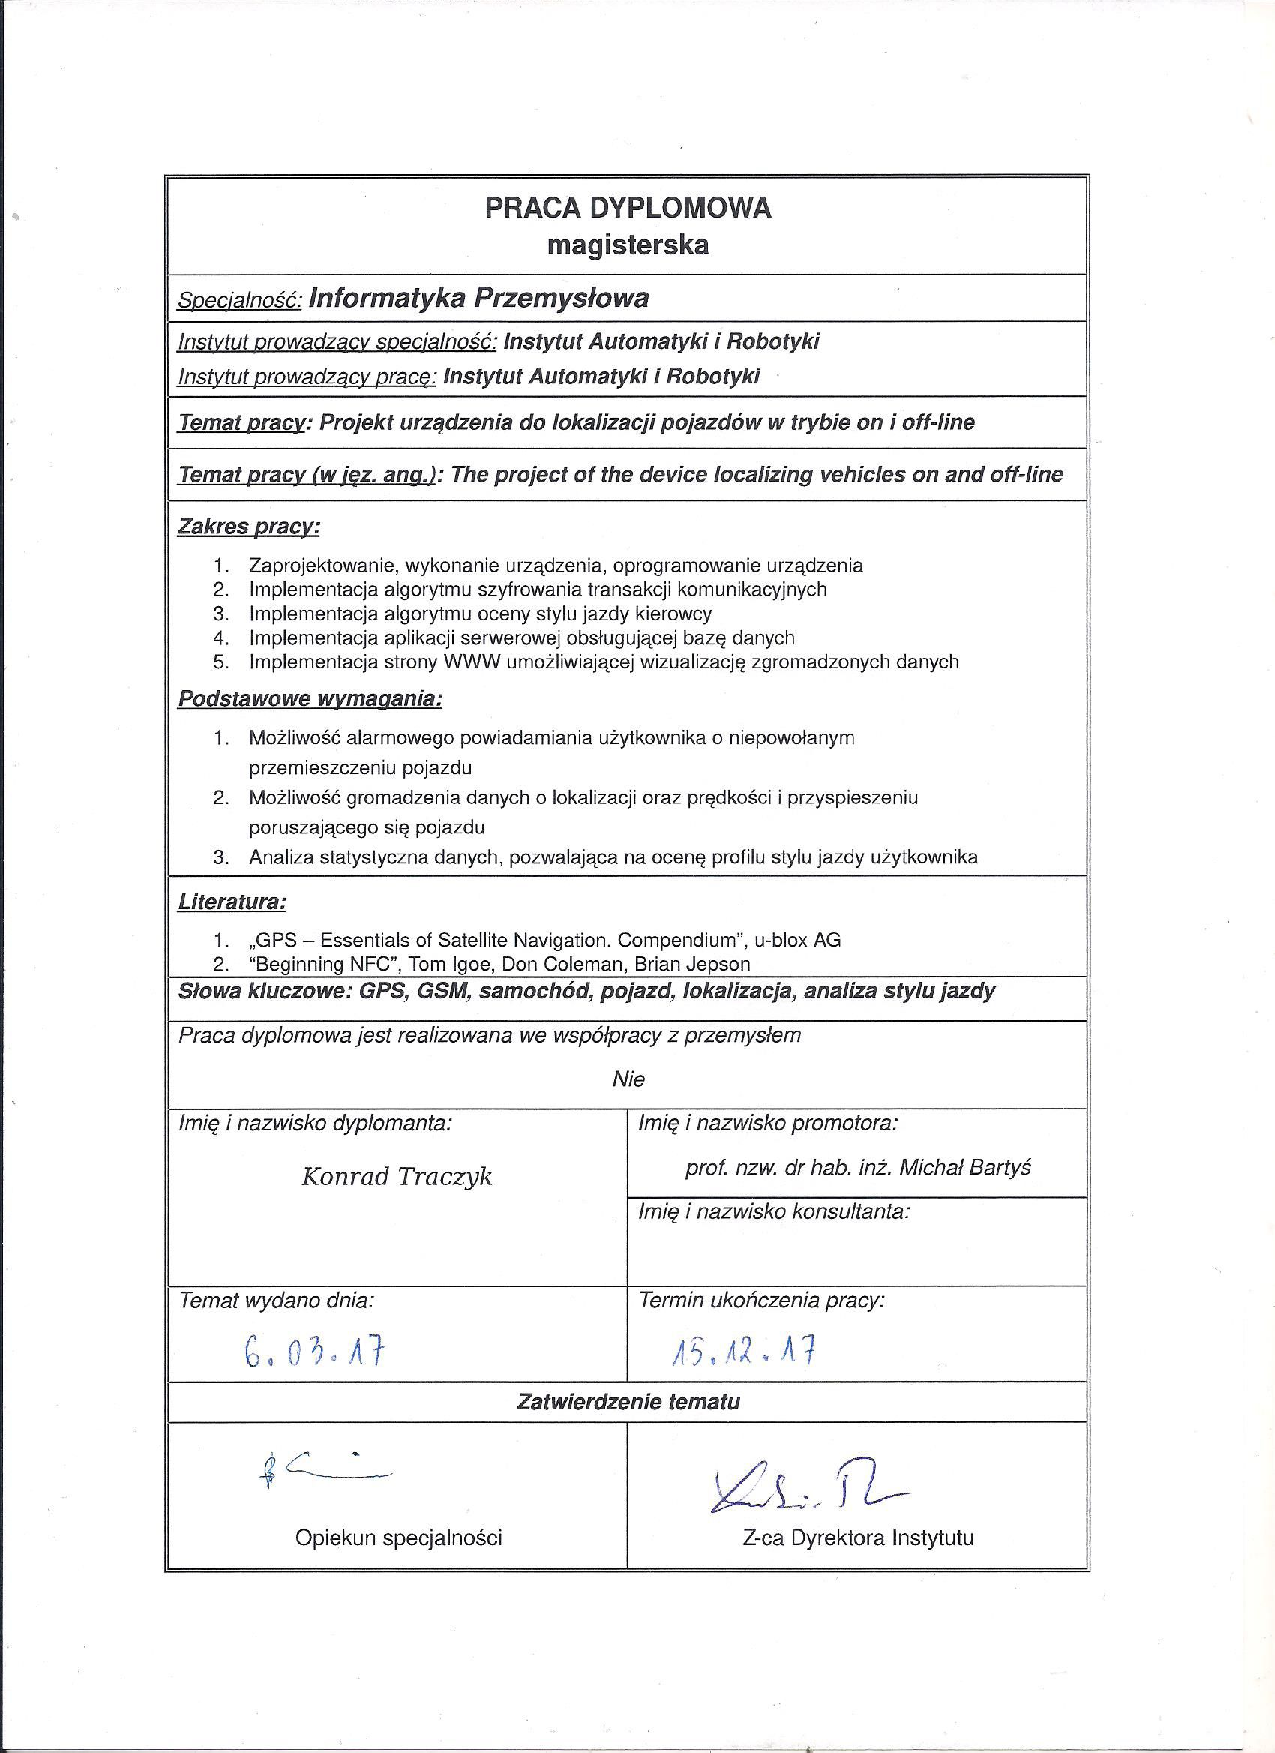
\includepdf[pages={1}]{chapters/Karta_Tematu_MGR.pdf}
\cleardoublepage

\thispagestyle{empty}
\noindent {\Large\textbf{Streszczenie}}\\

\noindent {\Large\textbf{Projekt urządzenia do lokalizacji pojazdów w trybie on i off-line}}\\

\begin{singlespacing}

Celem pracy było zaprojektowanie, wykonanie i oprogramowanie urządzenia stanowiącego dodatkowe zabezpieczenie pojazdu na wypadek kradzieży, w postaci lokalizatora wykorzystującego system GNSS (\textit{ang. Global Navigation Satellite System}) oraz GSM (\textit{ang. Global System for Mobile Communications}), zdolnego do analizy stylu jazdy kierowcy, a także całego systemu informatycznego, który pozwoliłby na obsłużenie pozyskanych danych. Założeniem jest, aby moduł elektroniczny mógł być zasilany z instalacji elektrycznej pojazdu, lecz poza tym był od niego całkowicie niezależny.\\

System opisywany w pracy przeznaczony jest głównie dla trzech grup osób. Pierwszą z nich są właściciele firm posiadających flotę pojazdów, prowadzonych przez pracowników. Umożliwia im zdalny podgląd tras przebywanych przez zatrudnione osoby, a także syntetyczną informację o sposobie jazdy kierowcy. Drugą kategorię stanowią osoby zainteresowane możliwością zdalnego zlokalizowania pojazdu w przypadku kradzieży, dzięki wykorzystaniu mechanizmu alarmowania poprzez wiadomości SMS. Ostatnia grupa to osoby, które chciałyby poprawić swoje umiejętności ekologicznego i bezpiecznego prowadzenia pojazdów, na podstawie dynamicznej oceny wydawanej przez lokalizator. \\

W skład systemu wchodzą dwa urządzenia elektroniczne. Jedno z nich służy do lokalizacji pojazdu, ciągłej oceny stylu jazdy, wysyłania danych na serwer, wykorzystując sieć GSM oraz awaryjnego powiadamiania właściciela w przypadku wykrycia kradzieży. Drugie urządzenie ma za zadanie autoryzować ruch pojazdu i deaktywować funkcję alarmu. Komunikacja pomiędzy obydwoma urządzeniami odbywa się zabezpieczonym kanałem poprzez Bluetooth Low Energy z wykorzystaniem algorytmu szyfrowania AES128. \\

Kolejnym elementem systemu jest aplikacja serwerowa napisana w języku C++. Jej celem jest odbieranie danych transmitowanych przez urządzenie, przetworzenie ich i zapisanie w bazie danych. Ponadto, jest ona odpowiedzialna za obsługę zapytań HTTP pochodzących ze strony internetowej, która stanowi ostatni moduł pracy. Jest ona wykorzystywana w celu rejestracji i logowania użytkowników do systemu, dodawania urządzeń, a także wyświetlania danych o przebytych trasach oraz ocenach stylu jazdy i ich wizualizacji na mapach od firmy Google. \\

W ramach pracy przeprowadzono również badania nad sposobem analizy i oceny stylu jazdy kierowcy, w oparciu o informacje dotyczące przyspieszenia i jego zmian pochodzące z akcelerometru. Badania zaowocowały przedstawieniem autorskiego algorytmu wykrywania agresywnego sposobu prowadzenia pojazdów. Wykonane samodzielnie testy drogowe wykazały jego skuteczność. \\

\textbf{Słowa kluczowe: }analiza stylu jazdy, Bluetooth Low Energy, GPS, GSM, lokalizacja, pojazd, samochód, szyfrowanie AES

\end{singlespacing}

\cleardoublepage
\thispagestyle{empty}

\noindent {\Large\textbf{Abstract}}\\


\noindent {\Large\textbf{The project of the device localizing vehicles on and off-line}}\\

\begin{singlespacing}


The main goal of this thesis is to design, build and program the device which is additional security module in case of vehicle's theft in the form of a GNSS (\textit{Global Navigation Satellite System}) and GSM (\textit{Global System for Mobile Communication}) system based locator with ability to analyze driving style of the vehicle user. Moreover, the aim was to create entire IT system for handling the gathered data. The assumption is that the electronic module is able to be powered by the vehicle's electrical system and yet still be completely independent. \\

The system described in the thesis is dedicated for three groups of recipients. The first one are owners of the companies that have vehicle's fleet which is used by the employees. It gives them the ability to remotely display the routes traveled by the employees along with the brief information about the driving style. The second category is the group of people interested in remote vehicle locating in case of the theft, thanks to the embedded alarming mechanism utilizing the SMS messages. The last group is made of customers who want to enhance their ecological driving skills based on the dynamically calculated driving style assessment. \\

The system consists of two electronic devices. The first one is used to locate vehicles,  continuously calculate driving style assessment, transmit the data on the web server via GSM network and notify the vehicle owner about the car theft. The function of the second device is to authorize the vehicle movement and deactivate the alarm feature. The communication between the devices relies on the secured channel based on the Bluetooth Low Energy protocol with usage of AES128 encryption algorithm. \\

The next part of the system is the server application written in C++ programming language. Its aim is to receive the data sent by the locator device, process it and store it in the database. Moreover, it is responsible for handling HTTP requests incoming from the website designed in the thesis. The website is used in order to register and authorize users, add devices and visualize the data regarding the traveled tracks and their assessments using the Google Map API. \\

Also, within this thesis the author conducted the research about the way of driving style analysis and assessment, based on the information about the acceleration and its changes received from the accelerator module used in the locator device. The experiments resulted in the proposition of the innovative algorithm to evaluate the driving style. Self-conducted road tests confirmed its efficiency. \\

\flushbottom
\textbf{Key words: }Bluetooth Low Energy, car, driving style analysis, GPS, GSM, localization, vehicle, AES encryption
\end{singlespacing}

\cleardoublepage


\includepdf[pages={1}]{chapters/Oswiadczenie_autora_pracy.pdf}
\cleardoublepage


\addcontentsline{toc}{chapter}{Spis treści}
\clearpage
\tableofcontents
\clearpage


\raggedbottom
\setpagenumberingtype{arabic} % kontynuowanie numerowania w stylu arabskim

\chapter{Wstęp}
\label{ch:wstep}

\section{Zakres pracy}
\label{project_sketch}
Celem pracy był projekt, wykonanie i oprogramowanie urządzenia stanowiącego dodatkowe zabezpieczenie pojazdu na wypadek kradzieży, w postaci lokalizatora wykorzystującego system GNSS (\textit{ang. \textbf{G}lobal \textbf{N}avigation \textbf{S}atellite \textbf{S}ystem}) oraz GSM (\textit{ang. \textbf{G}lobal \textbf{S}ystem for \textbf{M}obile Communications}), zdolnego do analizy stylu jazdy kierowcy, a także systemu informatycznego, który pozwoliłby na przetworzenie pozyskanych danych. Poza nim, w skład systemu informatycznego wchodzą:

\begin{itemize}
\item Strona WWW, umożliwiająca zdalny podgląd danych pochodzących z przypisanych do użytkownika urządzeń.
\item Aplikacja serwerowa, która obsługuje zapytania użytkownika oraz zapisuje napływające dane do bazy danych SQLite.
\end{itemize}

Do dodatkowych wymagań stawianych urządzeniu należą:

\begin{itemize}
\item Zapewnienie bezpiecznego szyfrowanego kanału komunikacji deaktywującej tryb alarmu.
\item Zaoewnienie zastępczego źródła zasilania, umożliwiającego pracę przy wyłączonym silniku pojazdu, bądź w razie odłączenia akumulatora.
\item Konstrukcja urządzenia o niewielkich wymiarach w celu umożliwienia łatwego ukrycia w pojeździe. 
\end{itemize}

Moduł umożliwia działanie w dwóch trybach. Pierwszy z nich polega na cyklicznym wysyłaniu na serwer pozycji i parametrów trakcyjnych samochodu w trakcie jego ruchu. Dzięki temu, możliwa jest między innymi zdalna ocena stylu jazdy kierowcy.

Drugi tryb jest aktywny w trakcie postoju i stanowi system alarmowego powiadamiania właściciela pojazdu o jego przemieszczeniu na przykład w przypadku kradzieży.

W celu zapewnienia bezpieczeństwa, postanowiono zrealizować projekt w postaci dwóch urządzeń. Jedno z nich – płytka lokalizatora, umożliwiająca lokalizację pojazdu oraz wysyłanie danych na serwer. Drugi moduł stanowi układ deaktywujący, którego zadaniem jest wyłączenie trybu alarmu po uruchomieniu samochodu przez upoważnioną do tego osobę. Obie płytki komunikują się ze sobą poprzez protokół Bluetooh Low Energy, zapewniający energooszczędną wymianę danych. Pozwala to na zasilenie układu deaktywującego z niewielkiej baterii i jego nieprzerwaną pracę nawet przez kilka lat bez konieczności wymiany źródła zasilania. 
Ponadto, aby umożliwić  bezpieczną transmisję danych, niezbędne jest zastosowanie mechanizmu szyfrowania. W celu eliminacji ryzyka podsłuchania procesu wymiany klucza szyfrującego, oba urządzenia zostały wyposażone w moduł NFC (\textit{ang. \textbf{N}ear \textbf{F}ield \textbf{C}ommunication}), zapewniającego bezkontaktową komunikację na odległość do 10 cm.
\clearpage
\section{Schemat blokowy}
\label{Schemat_blokowy_urządzen}
Na przedstawionym rysunku \ref{fig:image_device_block_diagram} zaprezentowano blokowy schemat funkcjonalny urządzeń, które stanowią główną część sprzętową projektu - moduł płyty głównej oraz moduł dezaktywatora. 

\begin{figure}[h]
	\centering
	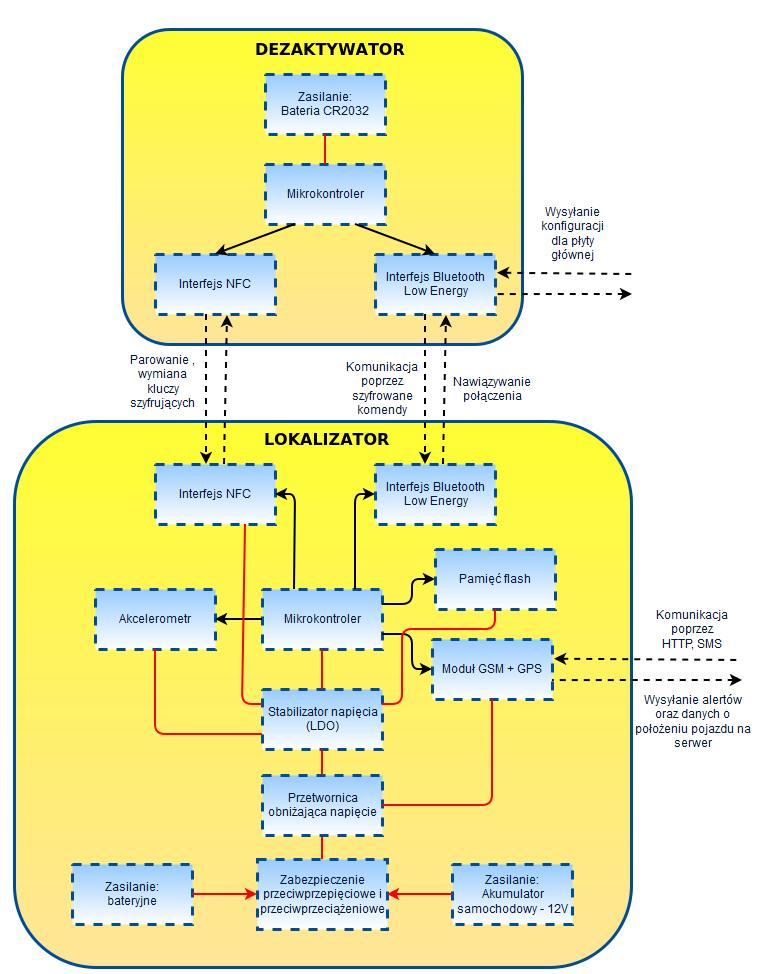
\includegraphics[width=13cm]{img/introduction/device_block_diagram.jpg}
	\caption{Schemat blokowy urządzeń wchodzących w skład systemu. \\ Źródło: Opracowanie własne.}
	\label{fig:image_device_block_diagram}
\end{figure}
	
	

\clearpage
\section{Istniejące rozwiązania}

W ramach pracy przeprowadzono analizę rynkową pod kątem istniejących, ciekawych rozwiązań. Poniżej zaprezentowano trzy najbardziej charakterystyczne z nich.

\begin{itemize}
\item Spark Nano 5.0 GPS Tracker

To przenośne urządzenie, posiadające zasilanie bateryjne i służące do śledzenia pozycji geograficznej przy pomocy systemu GPS. Zapewnia zdalne powiadamianie użytkownika o lokalizacji urządzenia poprzez sieć CDMA z dokładnością do 2m. Wymiary urządzenia: 64,5 x 40 x 20,5 mm. Urządzenie pozwala na działanie przez ok. 2 tygodnie, przy założeniu pracy przez 1 godzinę dziennie. Producent udostępnia platformę online oraz aplikacje na smartphony z systemem Android oraz IOS, do przedstawiania danych użytkownikowi. Urządzenie domyślnie raportuje położenie co minutę, lecz producent umożliwia zdalne zwiększenie częstotliwości w razie chęci użytkownika. Cena urządzenia: 129,99\$. Wizualizację urządzenia przedstawiono na rysunku \ref{fig:image_spark_nano_tracker}.
\begin{figure}[h]
	\centering
	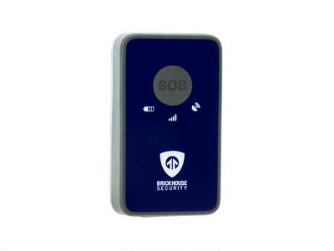
\includegraphics[width=7cm]{img/introduction/spark_nano.jpg}
	\caption{Spark Nano 5.0 GPS Tracker. Źródło: \cite{spark_nano}.}
	\label{fig:image_spark_nano_tracker}
\end{figure}

\item MyCarTracks - aplikacja mobilna

Jest to aplikacja na smartphona, która dodaje do niego funkcjonalność trackera GPS. Stanowi rozwiązanie typowo programowe, które wykorzystuje zasoby zawarte w telefonie – moduł GPS, GSM oraz internet. Jest ono proste i tanie, lecz nie pozbawione wad. Ponieważ to aplikacja na telefon, a nie osobne urządzenie, konieczne jest umieszczenie smartphone’a w pojeździe na stałe, jeśli użytkownik chciałby użytkować ją jako zabezpieczenie antykradzieżowe. Ponadto, telefony pobierają stosunkowo dużo energii co wymusza częste ich ładowanie. W rezultacie efektywne ukrycie urządzenia jest utrudnione. 
Do kosztów rozwiązania należy wliczyć cenę telefonu (używane urządzenie kosztuje ok. 200-300zł) oraz 7\$ za każdy pojazd miesięcznie. Aplikację przedstawiono na rysunku \ref{fig:image_my_car_tracks}.
\begin{figure}[h]
	\centering
	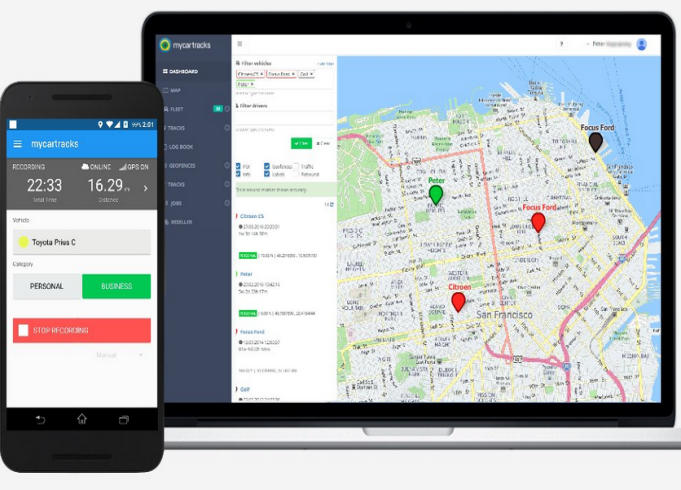
\includegraphics[width=7cm]{img/introduction/mycartracks.jpg}
	\caption{Aplikacja MyCarTracks. Źródło: \cite{my_car_tracks}.}
	\label{fig:image_my_car_tracks}
\end{figure}

\item STI GL300

Jest to kolejne niewielkie, przenośne urządzenie wykorzystujące moduł GPS do lokalizacji. Przekazuje ono informacje o położeniu w czasie rzeczywistym (co 60, 10 lub 5 sekund w zależności od wykupionej taryfy). Producent nie przedstawił informacji o sposobie komunikacji z serwerem, lecz najprawdopodobniej również wykorzystuje sieć GSM. Urządzenie to posiada baterię pozwalającą na ciągłą pracę do 2 tygodni. Przy tym nie ogranicza się ono jedynie do lokalizacji pojazdów dzięki niewielkim wymiarom. Producent wprowadza ciekawe funkcjonalności: powiadamianie poprzez wiadomość sms o osiągnięciu przez pojazd danej pozycji geograficznej, wejście w zdefiniowany obszar czy osiągnięcie pewnej prędkości. Aktualne oraz historyczne dane są przedstawiane użytkownikowi poprzez stronę internetową na mapach od firmy Google. Wymiary urządzenia to zaledwie ok. 5 cm x 2,5 cm x 2 cm.  W opcji dodatkowej można dokupić wodoodporną obudowę, pozwalającą na zamontowanie urządzenia na zewnątrz pojazdu. Cena urządzenia to 70\$ oraz od 25\$ do 40\$ miesięcznej opłaty. Wygląd urządzenia pokazano na rysunku \ref{fig:image_sti_gl300}.
\begin{figure}[h]
	\centering
	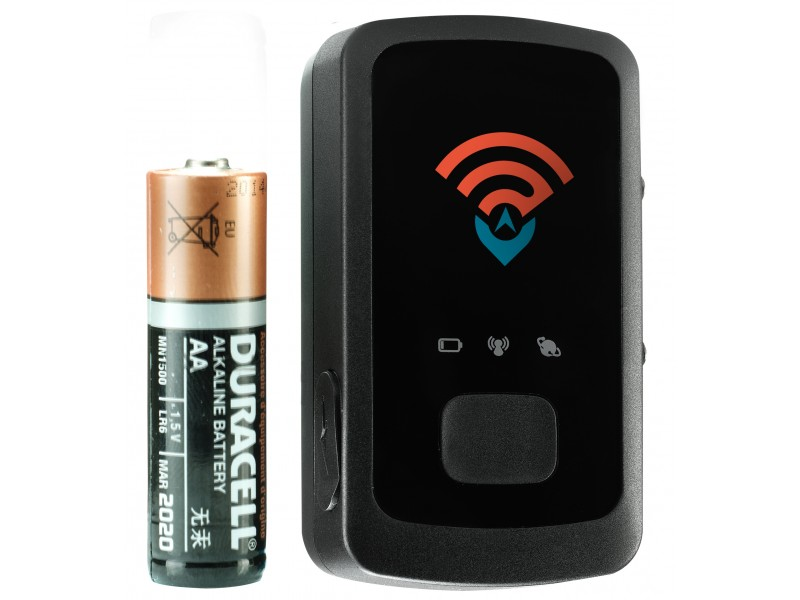
\includegraphics[width=7cm]{img/introduction/sti_gl300.jpg}
	\caption{Urządzenie STI GL300. Źródło: \cite{gl300}.}
	\label{fig:image_sti_gl300}
\end{figure}
\end{itemize}




%\clearpage{\pagestyle{empty}\cleardoublepage}

\chapter{Wstęp}
\label{teorethical_introduction}

\section{Zastosowane protokoły i systemy}
Dla realizacji celu pracy, zdecydowano się wykorzystać wymienione poniżej protokoły i interfejsy:
\begin{itemize}
	\item \textbf{GSM} - Wykorzystywany do komunikacji zdalnej dalekiego zasięgu (wysyłanie danych na serwer oraz komunikacja z użytkownikiem)
	\item \textbf{GPS} - Wykorzystywany do wyznaczenia lokalizacji pojazdu, a także jego prędkości oraz azymutu.
	
	\item \textbf{NMEA 0183} - Protokół w jakim moduł GPS wysyła dane do mikrokontrolera
	\item \textbf{Bluetooth Low Energy} - Wykorzystywany do komunikacji bliskiego i średniego zasięgu (komunikacja z użytkownikiem oraz z urządzeniem deaktywującym)
	\item \textbf{NFC} - Wykorzystywany do komunikacji bardzo bliskiego zasięgu (do wysłania klucza szyfrującego do oraz komendy deaktywującej z urządzenia deaktywującego)
\end{itemize}

Wszystkie z powyższych protokołów zostały pokrótce opisane, a następnie krótko zestawione.

\clearpage

\section{System GSM}
\label{GSM}

Poniższy podrozdział powstał na podstawie źródeł \cite{GSM}, \cite{GSM_tutorialspoint} oraz \cite{GSM_wiki}.\\

System GSM (\textit{ang. \textbf{G}lobal \textbf{S}ystem for \textbf{M}obile Communication}) jest obecnie najpowszechniej wykorzystywanym systemem służącym do komunikacji bezprzewodowej dalekiego zasięgu. System ten wykorzystywany jest do przesyłania głosu oraz serwisów danych. Pomysł na stworzenie sieci umożliwiającej komunikację głosową wyłonił się we wczesnych latach 70. ubiegłego wieku z opracowywanej w siedzibie Bell Laboratories mobilnej sieci radiowej. Jednakże dopiero dwanaście lat później, w 1982 roku powstał oficjalny komitet normalizacyjny nazwany \textit{Groupe Spécial Mobile}, którego zadaniem było utworzenie jednolitego, otwartego standardu dla telefonii komórkowej. 

Pierwotna wersja standardu działała w paśmie 900 MHz (880 - 960 MHz) i umożliwiała jedynie transmisję głosową. Jego kolejna wersja została opublikowana w 1990r. i definiowała ona dodatkowe pasmo 1800 MHz (1710 - 1880 MHz). Ponadto, umożliwiała przesyłanie krótkich wiadomości SMS (\textit{ang. \textbf{S}hort \textbf{M}essage \textbf{S}ystem}), a także faxu czy transmisję danych. Dalsze prace nad systemem wprowadziły do standardu techniki zwiększające przepustowość transmisji (maksymalna prędkość odbioru - 57.6 kb/s, maksymalna prędkość nadawania - 14.5 kb/s oraz 30 - 80 kb/s przy transmisji GPRS) oraz mechanizm przesyłania danych w pakietach GPRS (\textit{ang. \textbf{G}eneral \textbf{P}acket \textbf{R}adio \textbf{S}ervice}). 

Pomimo pojawienia się na świecie nowszych rozwiązań, takich jak sieci UMTS i LTE, ze względu na ogromną popularność, architektura sieci GSM wciąż jest rozwijana. 

System GSM umożliwia skorzystanie z następujących usług:
\begin{itemize}
	\item Połączenia głosowe - Stanowią one sztandarową funkcjonalność sieci GSM. Jej standard definiuje kodek GSM, który służy do zamiany głosu (skonwertowanego do napięciowego sygnału analogowego przez mikrofon) na postać cyfrową, która jest następnie kompresowana stratnie i transmitowana do odbiorcy. Stosowana jest kompresja na podstawie algorytmu LPC (ang. \textbf{L}inear \textbf{P}redictive \textbf{C}oding). Po stronie odbiorcy sygnał jest dekodowany, lecz ze względu na stratność LPC, słyszalny jest zniekształcony, nienaturalny głos rozmówcy.
	\item Transmisja danych - Umożliwia dostęp do internetu z urządzenia GSM, a także korzystanie z transmisji strumieniowej.
	\item Wiadomości tekstowe i multimedialne - Usługa przesyłania krótkich wiadomości tekstowych, o długości do 160 znaków, pod warunkiem korzystania jedynie z alfabetu łacińskiego. W przypadku stosowania znaków diakrytycznych maksymalny rozmiar wiadomości spada do 70 znaków. Wiadomości multimedialne (inaczej MMS), umożliwiają przesyłanie zdjęć, filmów czy dźwięków. Ich rozmiar maksymalny jest uzależniony od ograniczeń telefonu oraz operatora.
\end{itemize}

Jednym z głównych założeń systemu jest możliwość korzystania z niego przez wielu użytkowników jednocześnie. Aby rozwiązać ten problem, postanowiono zastosować technikę zmiany częstotliwości FDMA (\textit{ang. \textbf{F}requency \textbf{D}ivision \textbf{M}ultiple \textbf{A}ccess}) oraz okien czasowych TDMA (\textit{ang. \textbf{T}ime \textbf{D}ivision \textbf{M}ultiple \textbf{A}ccess}). Oznacza to, że pasmo częstotliwości GSM jest podzielone na wąskie kanały, o szerokości 200 kHz każdy. Czas użytkowania każdego kanału podzielony jest na 8 okien czasowych. Każde urządzenie ma zatem dostęp do sieci dostrajając się do odpowiedniego kanału w czasie trwania przydzielonego okna czasowego. Przedstawiono to na rysunku \ref{fig:image_gsm_frequencies_timeslots}.

\begin{figure}[H]
	\centering
	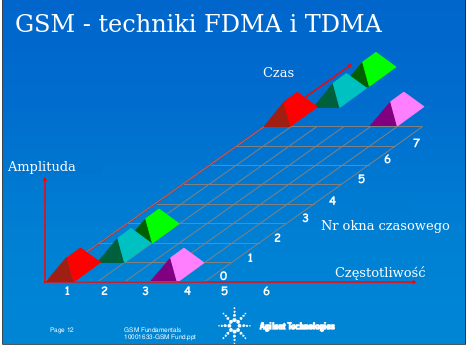
\includegraphics[width=8cm]{img/theory/GSM/gsm_timeslots_frequencies.png}
	\caption{Podział pasma częstotliwości na kanały i okna czasowe. Źródło: \cite{GSM}}
	\label{fig:image_gsm_frequencies_timeslots}
\end{figure}


Architektura sieci GSM powstała w oparciu o komórkowy system radiowy, skąd powszechnie stosowana nazwa - sieć komórkowa. Charakteryzuje się ona tym, że obszar terenu, na którym ma być prowadzona komunikacja radiowa dzieli się na tzw. komórki. Każdej komórce przypisana jest stacja bazowa (\textit{ang. \textbf{B}ase \textbf{T}ranceiver \textbf{S}tation}), która stanowi bramę dostępową do sieci. Urządzenie mobilne GSM, takie jak na przykład telefon, znajdując się na obszarze komórki najczęściej odbiera sygnał z więcej niż jednej stacji bazowej, jednakże zawiera połączenie z tą, której sygnał jest najsilniejszy. W razie spadku mocy sygnału stacji z którą urządzenie jest połączone, możliwa jest dynamiczna zmiana połączenia do innego BTS'a.

\begin{figure}[H]
	\centering
	
\includegraphics[width=8cm]{img/theory/GSM/cell_structure.png}
	\caption{Podział obszaru na komórki. Źródło: \cite{GSM_wiki}}
	\label{fig:image_gsm_cells}
\end{figure}

Aby móc korzystać z sieci GSM, urządzenia muszą posiadać kartę SIM (\textit{ang. \textbf{S}ubscriber \textbf{I}dentification \textbf{M}odule}). Oprócz przydatnych dla użytkownika wbudowanej pamięci na wiadomości SMS i kontakty, posiada unikalny na całym świecie numer identyfikujący użytkownika w sieci. W celu zalogowania się do sieci, urządzenie GSM musi podać ten numer w trakcie nawiązywania połączenia ze stacją bazową. 

Każda stacja bazowa wykorzystuje wiele kanałów GSM. Jednakże, aby nie dopuścić do wzajemnego zakłócania się, stacje bazowe z przylegających do siebie cel wykorzystują inne zbiory kanałów. Dodatkowo, w stacjach bazowych stosuje się dwa rodzaje anten - dookólne i kierunkowe o pokryciu 120\degree. Anteny dookólne pokrywają caly obszar komórki tym samym zbiorem kanałów, natomiast kierunkowe - dla każdego podobszaru wykorzystują ich inny zestaw. Ze względu na skończoną prędkość sygnału radiowego, istnieje również maksymalny promień pojedynczej komórki. W praktyce wynosi on około 35 km. Poniważ istnieje konieczność umożliwienia prowadzenia komunikacji na tak duży zasięg, standard ten nie należy do najbardziej energooszczędnych. W zależności od klasy urządzenia, minimalna moc nadawanego sygnału może wynosić od 1 do 20 mW, natomiast maksymalna nawet do 8 W. Urządzenia GSM mają możliwość dostosowywania mocy transmisji na podstawie mocy sygnału odebranego od stacji bazowej, w celu ograniczenia  wysokiego zużycia energii. 

Biorąc jednak pod uwagę fakt, iż transmisja przebiega w oknach czasowych, moc średnia jest niższa. Każde okno czasowe trwa 577 $\mu s$, a w jego czasie można wysłać jedną z kilku ramek komunikacyjnych. W trakcie każdej z nich można wysłać 148 bitów danych. W przypadku ramki nadawanej w trakcie rozmowy, głos kodowany jest jedynie na 57 bitach. Każde z urządzeń w sieci otrzymuje okno czasowe co 4.615 ms, liczone od początku okna, do rozpoczęcia następnego. Stąd wynika, że  w trakcie nadawania, urządzenie transmituje dane jedynie przez 12.5\% czasu. Pobór prądu, w zależności od odległości do nadajnika, a więc od mocy nadawania, może wówczas wynosić nawet do 1.5 A. Przyjmując napięcie zasilania układu GSM wynoszące 4 V, maksymalna pobierana moc średnia może wynosić:

\begin{gather}
 	P_{\text{śr}} = U \cdot I \cdot \tau \\
 	P_{\text{śr}} = 4 V \cdot 1.5 A \cdot 0.125 = 0.75 W \nonumber 	
 	\label{eq_gsm_power_mean} 
\end{gather}
 gdzie:
 
 $P_{\text{śr}} $ - moc średnia
 
 $U$ - napięcie zasilania układu,
 
 $I$ - nateżęnie prądu w momencie transmisji
 
 $\tau$ - współczynnik wypełnienia impulsu (czas trwania okna czasowego podzielony przez czas pomiędzy oknami czasowymi)
 
Wartość mocy średniej wynosząca 0.75 W odpowiada ciągłemu zużyciu prądu rzędu 187.5 mA przy napięciu zasilania układu rzędu 4 V. 




\section{System GPS}
\label{GPS}

Poniższy podrozdział powstał na podstawie źródeł \cite{GPS_ublox} oraz \cite{inzynierka}.\\



System GPS(\textit{ang. \textbf{G}lobal \textbf{P}ositioning \textbf{S}ystem}) był historycznie pierwszym systemem nawizgacji satelitarnej GNSS (\textit{ang. \textbf{G}lobal \textbf{N}avigation \textbf{S}attelite \textbf{S}ystem}). Powstał w wyniku prac w Departamencie Obrony Stanów Zjednoczonych i jest w pełni własnością rządu tego kraju. Oprócz niego istnieją jeszcze rosyjski GLONASS, a od niedawna europejski Galileo oraz chiński Beidou. Ostatnie dwa systemy satelitarne nie są jeszcze w pełni funkcjonalne, stanowią raczej systemy o zasięgu regionalnym niż globalnym.

Głównym elementem składowym systemów nawigacji satelitarnej, są jak sama nazwa wsazuje satelity. Poruszają się one po ściśle określonych, stałych orbitach, które są tak dobrane, aby z dowolnego punktu na globie, w dowolnym momencie była możliwość odebrania sygnału z co najmniej czterech z nich. Przedstawia to rysunek \ref{fig:image_gps_basics}.

\begin{figure}[H]
	\centering
	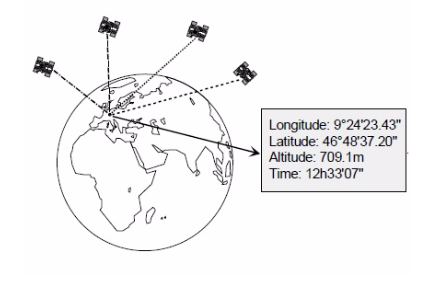
\includegraphics[width=10cm]{img/theory/GPS/gps_introduction.png}
	\caption{Model działania systemu GPS. Źródło: \cite{GPS_ublox}}
	\label{fig:image_gps_basics}
\end{figure}

Podstawę w systemach GNSS stanowi czas. Każdy z satelitów posiada 4 zegary atomowe, które stanowią najdokładniejsze źródło czasu znane ludzkości. Zegary te posiadają błąd rzędu 1 sekundy po upływie najwcześniej 30000 lat. Dodatkowo, są one co pewien czas synchronizowane ze źródłami na Ziemi.

Zadaniem każdego z satelitów jest nadawanie w formie rozgłoszeniowej sygnału, w którym zawarta jest wiadomość o jego lokalizacji na orbicie oraz czasie w momencie wysyłania wiadomości. Sygnał ten nadawany jest drogą radiową więc jego prędkość jest równa prędkości światła. Po dotarciu do odbiornika jest on bardzo słaby, przez co praktycznie niemożliwe jest jego odebranie wewnątrz budynków, a w pobliżu wysokich obiektów dokładność lokalizacji spada. Najdokładniejsze wyniki wyznaczania pozycji można osiągnąć na otwartej przestrzeni. Podstawowy sygnał przesyłany jest na fali nośnej o częstotliwości 1575.42 MHz i nosi nazwę L1.

Ponadto, sygnał GPS (a także pochodzący z innych systemów lokalizacji satelitarnej) ulega łatwo zakłóceniom w momencie przejścia przez jonosferę, bowiem fala elektromagnetyczna ulega na niej załamaniu, przez co zmienia swój tor i wydłuża drogę. W efekcie, pomiary odległości od odbiornika do satelity, niezbędne do wyznaczenia lokalizacji przestają być dokładne i pojawia się błąd lokalizacji.
Problem ten rozwiązano na 2 sposoby. Pierwszym z nich jest nadawanie sygnału przez satelity na kilku częstotliwościach. Każda z nich, przechodząc przez jonosferę ulega załamaniu, lecz pod innym kątem, przez co pokonają różne długości drogi przebytej do odbiornika, a tym samym zostaną odebrane w różnych momentach. Dzięki temu, odbiornik jest w stanie wyznaczyć korektę i wyeliminować błąd. Pierwotnie, rozwiązanie to było dostępne jedynie w celach militarnych, lecz od 2005 roku, Departament Obrony Stanów Zjednoczonych udostępnił częstotliwość L2 (1227.60 MHz) do celów cywilnych, a od 2008r. - również L5 (1176.45 MHz). Częstotliwości dostępne w systemie GPS pokazano na rysunku \ref{fig:image_gps_frequencies}.

\begin{figure}[H]
	\centering
	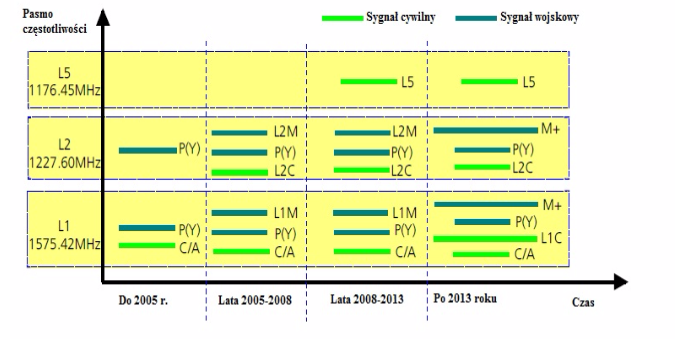
\includegraphics[width=15cm]{img/theory/GPS/gps_frequencies.png}
	\caption{Zbiór częstotliwości wykorzystywanych w systemie GPS. Źródło: \cite{inzynierka}}
	\label{fig:image_gps_frequencies}
\end{figure}

Druga metoda to wyznaczenie korekty dla przejścia przez jonosferę w stacjach naziemnych, a następnie rozgłaszanie depeszy ją zawierającej poprzez sieć stacji bazowych. Rozwiązanie to nosi miano DGPS (\textit{ang. \textbf{D}ifferential \textbf{GPS}}). Dzięki zastosowaniu tej techniki, dokładność lokalizacji wzrasta z nominalnych 15 m nawet do 10 cm.

Układy GPS, które umożliwiają skorzystanie z któregoś z tych dwóch rozwiązań są jednak kosztowne, więc na rynku cywilnym najpowszechniej stosowane są moduły wykorzysujące jedynie częstotliwość L1. Dzięki temu, za kilkadziesiąt złotych można uzyskać system z dokładnością do kilku metrów w sprzyjających warunkach \cite{inzynierka} (Rozdział 7 - Testy urządzenia). W pracy tej uzyskano dokładność systemu rzędu 1 - 2 metrów przy braku zakłóceń, oraz 5 - 7 metrów idąc wzdłuż wysokich budynków.

Aby zrozumieć zasadę działania systemu GPS proszę wyobrazić sobie sytuację jak na rysunku \ref{fig:image_gps_basics1}:

\begin{figure}[H]
	\centering
	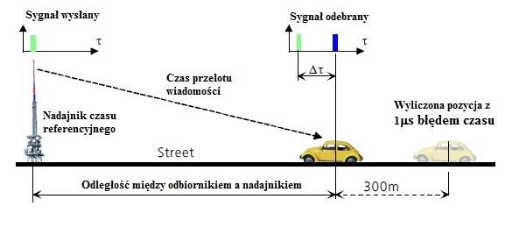
\includegraphics[width=12cm]{img/theory/GPS/gps_basics1.png}
	\caption{Zasada działania systemu GPS. Źródło: \cite{inzynierka}}
	\label{fig:image_gps_basics1}
\end{figure}

Załóżmy, że w przedstawionym pojeździe znajduje się odbiornik GPS. W pewnym momencie odbiera on sygnał GPS z nadajnika referencyjnego. W sygnale znajduje się wartość czasu w momencie wysłania wiadomości. Ze względu na skończoną prędkość światła ($c = 299 792 458 m/s$), zostanie ona odebrana przez odbiornik z pewnym opóźnieniem. Wykorzystując ten fakt i znając prędkość transmisji (wartość prędkości światła), można wyznaczyć odległość do nadajnika:

\begin{equation}
	D = c \cdot \Delta t
\end{equation}

gdzie,

$D$ - odległość między nadajnikiem i odbiornikiem

$c$ - prędkość światła

$\Delta t$ - różnica czasu między wysłaniem i odebraniem wiadomości

Aby wyznaczyć różnicę czasu, odbiornik powinien mieć również własny zegar. Powinien on być przy tym niezwykle dokładny i zsynchronizowany z zegarem w nadajniku, bowiem błąd rzędu 1 $\mu s$ powoduje błąd lokalizacji rzędu 300 m. Ponieważ uzyskanie takiej dokładności oraz synchronizacji w każdym odbiorniku jest niemożliwe, należało znaleźć sposób umożliwiający rezygnację z konieczności posiadania zegara w odbiorniku. Przedstawiono go na rysunku \ref{fig:image_gps_basics2}:

\begin{figure}[H]
	\centering
	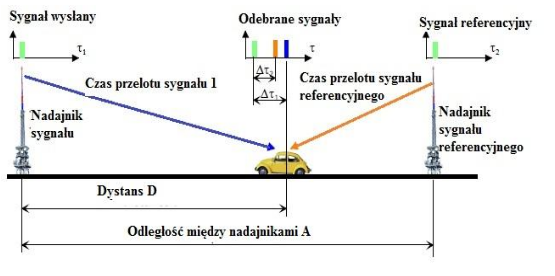
\includegraphics[width=12cm]{img/theory/GPS/gps_basics2.png}
	\caption{Zasada działania systemu GPS - sygnał referencyjny. Źródło: \cite{inzynierka}}
	\label{fig:image_gps_basics2}
\end{figure}

Polega on na zastosowaniu dodatkowego sygnału referencyjnego czasu. Wówczas po odebraniu obu sygnałów (które zostały wysłane w tym samym momencie) otrzymujemy:

\begin{equation}
\begin{cases}
\Delta \tau_1 \cdot c = D \\ 
\Delta \tau_2 \cdot c = A - D
\end{cases}
\end{equation}

Gdzie:

$\tau_1$ - różnica czasu między wysłaniem sygnału z nadajnika, a momentem jego odebrania

$\tau_2$ - różnica czasu między wysłaniem sygnału z nadajnika referencyjnego, a momentem jego odebrania

$A$ - odległość między nadajnikami

$D$ - odległość od nadajnika do odbiornika\\

Po odjęciu od pierwszego równania drugiego otrzymamy:

\begin{gather}
(\Delta \tau_1  - \Delta \tau_1) \cdot c = 2D - A \\
D = \frac{(\Delta \tau_1  - \Delta \tau_1) \cdot c + A}{2} \nonumber 
\end{gather}

Ponieważ jednak:

\begin{equation}
\begin{cases}
	\Delta \tau_1 = t - \tau_1 \\
	\Delta \tau_2 = t- \tau_2
\end{cases}
\end{equation}

to

\begin{equation}
(\Delta \tau_1 - \Delta \tau_2) = ((t - \tau_1) - (t - \tau_2)) = \tau_2 - \tau_1
\end{equation}

Gdzie:

$t$ - czas w momencie nadania sygnału przez nadajniki

$\tau_1$ - różnica czasu między wysłaniem sygnału z nadajnika, a momentem jego odebrania

$\tau_2$ - różnica czasu między wysłaniem sygnału z nadajnika referencyjnego, a momentem jego odebrania

Powyższe równania prowadzą do wniosku, że zastosowanie dodatkowego nadajnika referencyjnego, zsynchronizowanego z satelitami powoduje eliminację konieczności posiadania zegara w odbiorniku.

W rzeczywistości, takim nadajnikiem referencyjnym jest inny satelita GPS, bowiem są one ze sobą zsynchronizowane i nadają w dokładnie tym samym momencie.

Wyznaczona powyżej odległość $D$ dotyczy odcinka (jednej współrzędnej), a w rzeczywistości do wyznaczenia lokalizacji, uwzględniając satelitę referencyjnego, potrzeba sygnału z co najmniej 4 satelitów.



\section{Protokół NMEA 0183}
\label{NMEA}

Niniejszy podrozdział powstał na podstawie źrodeł \cite{inzynierka} oraz \cite{QUECTEL_HW_DESIGN}.\\

Protokół ten stanowi standard komunikacji między urządzeniami elektronicznymi wykorzystywanymi w urządzeniach morskich, zwłaszcza urządzeniami do lokalizacji i nawigacji. Zawiera on specyfikację elektryczną oraz opis ramek (wiadomości) wymienianych między modułami. Powstał w Stanach Zjednoczonych w \textit{\textbf{N}ational \textbf{M}arine \textbf{E}lectronics \textbf{A}ssociation}. Jego najnowsza, czwarta wersja pochodzi z listopada 2008 roku. 
Protokół ten pierwotnie wykorzystywał interfejs RS232, lecz w wersji drugiej dokonano jego zmiany na RS422. Interfejsy te różnią się jedynie poziomami napięć przypisanym logicznym wartościom bitów 0 i 1. 
Oba z nich umożliwiają wysyłanie danych bajt po bajcie. Każdy z nich rozpoczyna się bitem START (stan niski w RS422), który umożliwia odbiornikowi wykrycie początku bajtu i synchronizację. Następnie wysłanych jest kolejno 8 bitów danych, po których przesyłany jest bit parzystości (0 gdy liczba bitów w bajcie danych o wartości 1 jest parzysta lub 1 gdy jest nieparzysta) i na koniec - bit stopu. Przedstawiono to na rysunku \ref{fig:image_nmea_rs422}.

\begin{figure}[H]
	\centering
	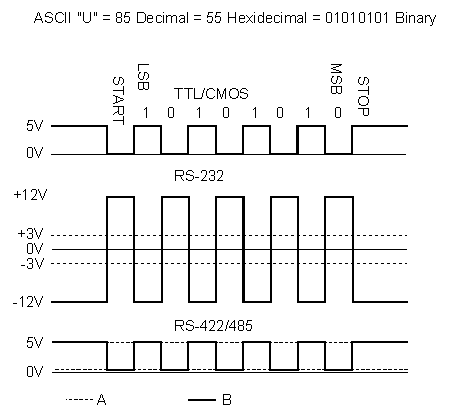
\includegraphics[width=10cm]{img/theory/NMEA/RS232_RS422.png}
	\caption{Poziomy napięć i kolejnośc bitów w interfejsach RS232 i RS422. Źródło: \cite{RS422}}
	\label{fig:image_nmea_rs422}
\end{figure}

Na podstawie tego interfejsu, NMEA nabudowała wyższą warstwę protokołu w postaci wiadomości. Każda wiadomość rozpoczyna się symbolem '\textbf{$\$$}', po którym występuje 2 literowy kod mówiący o type urządzenia (GP - urządzenie GPS, GN - urządzenie GLONASS) i 3 literowy kod definiujący typ przesyłanej wiadomości. Po kodzie występuje przecinek, a następnie lista pól danych oddzielonych przecinkami. W obrębie wiadomości, każde pole ma ściśle określoną funkcję i w razie nie występowania, musi zostać przesłane jako puste. Za ostatnim polem występuje znak '\textbf{*}', po którym znajduje się suma kontrolna, liczona jako funkcja Exclusive Or (XOR) ze wszystkich znaków między '\textbf{$\$$}', a '\textbf{*}' bez ich uwzględnienia. 

Lista zdefiniowanych wiadomości jest bardzo długa, jednak w tabeli \ref{table:table_nmea_messages} zestawiono najpowszechniej wykorzystywane w odbiornikach GPS.

\begin{table}[H]
\centering
\caption{Najczęściej wykorzystywane wiadomości NMEA0183 w odbiornikach GPS.\\ Źródło: \cite{inzynierka}}
\label{table:table_nmea_messages}
\begin{tabular}{| l | l |}
\hline
GGA & Najczęściej wykorzystywane dane związane z ustalaniem pozycji GPS \\  \hline
GGL & Pozycja geograficzna – długość, szerokość \\  \hline
GSA & Informacje o aktywnych satelitach oraz o jakości połączenia \\ 
    & (DOP – \textit{ang.    Dilution of Position}) \\ \hline
GSV & Informacje o satelitach w zasięgu \\ \hline
RMC & Rekomandowane minimum danych GNSS \\ \hline
VTG & Dane o kursie oraz prędkości \\ \hline
ZDA & Wiadomość z aktualnym czasem i datą \\ \hline
\end{tabular}
\end{table}

W niniejszej pracy, aby zrealizować założenia projektu niezbędne było sparsowanie (przeanalizowanie) danych z dwóch wiadomości nadawanych przez moduł GPS: GGA i VTG.
Z wiadomości GGA  wyłoniono informacje o długości i szerokości geograficznej, wskaźnikach półkul, statusie wyznaczenia lokalizacji, jakości odebranego sygnału, liczbie satelitów w zasięgu oraz wysokości nad poziomem morza. Wiadomość VTG została wykorzystana w celu uzyskania informacji o kursie (azymucie) oraz prędkości odbiornika. Ich struktury przedstawiono kolejno w tabelach \ref{table:table_nmea_gga_message} i \ref{table:table_nmea_vtg_message}.

\begin{table}[H]
\centering
\caption{Struktura wiadomości GGA. Źródło: Twórczość własna}
\label{table:table_nmea_gga_message}
\begin{tabular}{| l | l |}
\hline
\textbf{Pole} & \textbf{Opis} \\ \hline
\$ & Symbol początku wiadomości  \\ \hline
GP & Typ urządzenia  \\ \hline
GGA & Typ wiadomości  \\ \hline
130305.743 & Czas UTC w formacie hhmmss.sss \\ \hline
4717.115 & Szerokość geograficzna w formacie ddmm.mmm \\ \hline
N & Wskaźnik półkuli (N - północna, S - południowa) \\ \hline
00833.912 & Długość geograficzna w formacie dddmm.mmm  \\ \hline
E & Wskaźnik półkuli (W - zachodnia, E - wschodnia) \\ \hline
1 & Wskaźnik informujący o statusie wyznaczania pozycji \\ 
 & 0 - pozycja nieustalona \\ 
 & 1 - pozycja ustalona na podstawie sygnału z satelitów \\ 
 & 2 - pozycja ustalona przy pomocy DGPS \\ 
 & 6 - pozycja wyestymowana za pomocą mechanizmu \textit{Dead reckoning} \\ \hline
08 & Liczba satelitów z których odebrano sygnał \\ \hline
0.94 & Wskaźnik jakości sygnału (0.5 - najlepsza, 20 - bardzo niska) \\ \hline
00499 & Wysokość nad poziomem morza \\ \hline
M & Jednostki wysokości (M - metry) \\ \hline
047 & Różnica w wysokości między geoidą (Ziemią), a elipsoidą (przybliżeniem Ziemi) \\ \hline
M & Jednostki wysokości (M - metry) \\ \hline
,, & Dane DGPS (pole puste) \\ \hline
0000 & Numer identyfikacyjny stacji bazowej DGPS \\ \hline
* & Znak końca danych \\ \hline
58 & Suma kontrolna \\ \hline
$<$CR$><$LF$>$ & Znak końca wiadomości \\ \hline
\end{tabular}
\end{table}

\begin{table}[H]
\centering
\caption{Struktura wiadomości VTG. Źródło: Twórczość własna}
\label{table:table_nmea_vtg_message}
\begin{tabular}{| l | l |}
\hline
\textbf{Pole} & \textbf{Opis} \\ \hline
\$ & Symbol początku wiadomości  \\ \hline
GP & Typ urządzenia  \\ \hline
VTG & Typ wiadomości  \\ \hline
227.15 & Kurs (azymut) w stopniach \\ \hline
T & Pole stałe, zawierające symbol T \\ \hline
,, & Kurs magnetyczny (nie zaimplementowany przez producenta) \\ \hline
M & Pole stałe, zawierające symbol M \\ \hline
0.00 & Prędkość \\ \hline
N & Pole stałe opisujące jednostki prędkości (N - węzły, K - kilometry na godzinę) \\ \hline
0.00 & Prędkość \\ \hline
K & Pole stałe opisujące jednostki prędkości (N - węzły, K - kilometry na godzinę) \\ \hline
A & Tryb pozycjonowania \\
  & N - brak pozycji \\
  & A - pozycja na podstawie sygnału z satelitów \\
  & D - pozycja na podstawie DGPS \\ \hline
* & Znak końca danych \\ \hline
3E & Suma kontrolna \\ \hline
$<$CR$><$LF$>$ & Znak końca wiadomości \\ \hline
\end{tabular}
\end{table}



\section{Protokół Bluetooth Low Energy}
\label{bluetooth}

Poniższy podrozdział powstał na podstawie źródeł \cite{BLE} oraz \cite{inzynierka}.\\

Projekt protokołu BLE (\textit{ang. \textbf{B}luetooth \textbf{L}ow \textbf{E}nergy}) został zapoczątkowany przez firmę Wibree należącą do grupy Nokia. Celem nadrzędnym, który przyświecał jego autorom nie było utworzenie kolejnego protokołu, którego zastosowanie byłoby przesadnie szerokie. Zamiast tego, zdecydowali się oni na zaprojektowanie standardu radiowego umożliwiającego najniższe możliwe zużycie energii, a przy tym nieskomplikowanego, przez co możliwe byłoby zastosowanie go w systemach o niskich kosztach budowy. Innymi słowy są to założenia idealne dla rynku smartfonów oraz IoT (\textit{ang. \textbf{I}nternet \textbf{o}f \textbf{T}hings}), gdzie urzadzenia zasilane są z niewielkich baterii (często CR2032). Dla przykładu, zakup w liczbie 1000 sztuk mikrokontrolera użytego w tej pracy - nRF52832 wyprodukowanego przez Nordic Semiconductor, który posiada wbudowany stos BLE, kosztuje jedynie 9.78 zł za sztukę.

W trakcie prac, projekt zostął przejęty przez grupę Bluetooth SIG (\textit{ang. \textbf{B}luetooth \textbf{S}pecial \textbf{I}nterests \textbf{G}roup}), zrzeszającą dziesiątki firm i organizacji z wielu dziedzin przemysłu, zainteresowanych wykorzystywaniem i rozwojem protokołu Bluetooth. W roku 2010, Bluetooth Low Energy, znany również jako Bluetooth Smart został włączony do standardu Bluetooth 4.0, obok klasycznego protokołu Bluetooth Classic. Nie należy jednakże mylić tych dwóch protokołów komunikacyjnych, ponieważ poza warstwą fizyczną (interfejs radiowy o częstotliwości 2.4 GHz w pasmie ISM) różnią się w swych założeniach. Bluetooth Classic jest bowiem typowym protokołem umożliwiającym szybką, lecz energochłonną komunikację. W grudniu 2013 roku wprowadzono pierwszą dużą poprawkę do protokołu (Bluetooth 4.1), a rok później dalsze modyfikacje w postaci standardu Bluetooth 4.2. 

Bluetooth Low Energy, ze względu na swoje założenie o onergoszczędności posiada pewne ograniczenia. Pierwszym z nich jest przepustowość danych. Górna granica prędkości transmisji wynosi 1 Mb/s, jednakże jest to wartość jedynie teoretyczna. W praktyce jest ona obwarowana wieloma ograniczeniami sprzętowymi producentów mikrokontrolerów. W standardzie zawarte jest, iż pojedynczy pakiet danych może zawierać maksymalnie 20 bajtów. Ograniczenie sprzętowe wynika tu z częstotliwości wysyłania pakietów. Dla  mikrokontrolera Nordic Semiconductor z rodziny nRF51, wynosi ona do 6 pakietów na każdy interwał połączenia. Jest to konfigurowalny parametr, określający odcinek czasu w obrębie którego jeśli nie dojdzie do transmisji pakietu, połączenie zostanie uznane za zerwane. Interwał połączenia może wynosić od 7.5 ms do 4 s. Przy założeniu najkrótszej wartości tego parametru otrzymujemy przepustowość:

\begin{equation}
	\text{Przepustowość} = 6 \text{pakietów/interwał} \cdot \frac{1000ms}{7.5ms} \cdot 20 \text{bajtów} = 15960 \text{bajtów/s} \approx 128 kb/s
\end{equation}

Jak widać jest to wartość znacznie odbiegająca od 1 Mb/s, jednakże w porównaniu do zysku na zużyciu energii jest to i tak bardzo dobry wynik. 

Kolejne ograniczenie to zasięg komunikacji. Oficjalnie, Bluetooth Low Energy posiada zasięg rzędu 50 m. Jest to jednak wartość trudna do uzyskania, silnie zależna od otoczenia (między urządzeniami nie może być przeszkód), mocą transmisji (rekonfigurowalna, im mniejsza tym zasięg mniejszy) oraz liczbą innych urządzeń znajdujących się w pobliżu, która to decyduje o zajętości kanałów. Pasmo częstotliwości (od 2.402 GHz do 2.480 GHz) wykorzystywanej przez protokół podzielone jest bowiem na 40 kanałów. Przedstawiono to na rysunku \ref{fig:image_ble_channels}.

\begin{figure}[H]
	\centering
	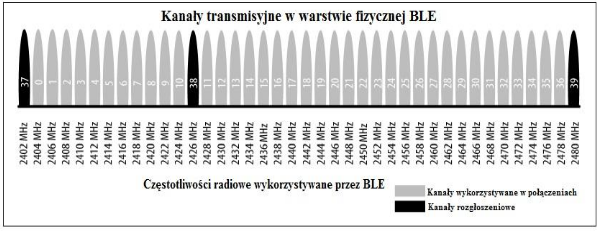
\includegraphics[width=17cm]{img/theory/BLE/ble_channels.png}
	\caption{Struktura pasma 2.4 ISM wykorzystywanego przez Bluetooth Low Energy.\\Źródło: \cite{inzynierka}}
	\label{fig:image_ble_channels}
\end{figure}

Protokół Bluetooth Low Energy oferuje dwie możliwości wysyłania danych. Pierwszym z nich jest bezpołączeniowe rozgłaszanie (\textit{ang. Advertising}). Wówczas, każde z urządzeń wysyła cyklicznie  w eter pakiet danych o pojemności do 31 bajtów. Interwał między pakietami może wynosić od 20 ms do 10.24 s. Jest to jednak komunikacja jednokierunkowa. Wysłane w ten sposób dane może odebrać każde urządzenie będące w zasięgu.

\begin{figure}[H]
	\centering
	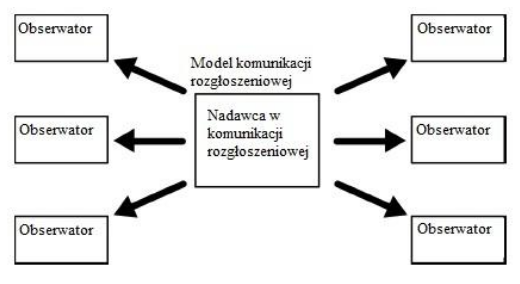
\includegraphics[width=12cm]{img/theory/BLE/ble_advertising.png}
	\caption{Model komunikacji rozgłoszeniowej. Źródło: \cite{inzynierka}}
	\label{fig:image_ble_advertising}
\end{figure}

Drugą metodą jest wysyłanie danych będąc w połączeniu. Wówczas komunikacja może być obustronna. W tym przypadku, BLE definiuje dwa możliwe typy urządzeń. Jedno z nich, które inicjuje połączenie określane jest jako \textit{Central}, natomiast urządzenie akceptujące połączenie - \textit{Peripheral}. Nie występuje przy tym ograniczenie, że urządzenie może mieć tylko jedną rolę. Może ono będąc w połączeniu urządzeniem typu \textit{Peripheral} zainicjować samodzielnie połączenie z innym odbiornikiem, a więc stać się dla tego połączenia\textit{Central'em}. Ważne jest, że urządzenie posiada jedną rolę dla danego połączenia, które jest realizowane typu punkt - punkt. 

Standard Bluetooth Low Energy definiuje logiczny podział struktur danych. Główną jednostką są tak zwane serwisy. Są to zgrupowania pewnych funkcjonalności, zwanych charakterystykami. Charakterystyki stanowią podstawowe jednostki komunikacji. Mogą one zawierać tzw. deskryptory, które są krótkimi, zrozumiałymi dla ludzi informacjami jak na przykład nazwa charakterystyki. Można to porównać do definicji klasy (serwis), zawierającej definicje metod (charakterystyk). Struktura ta zarzadzana jest przez tak zwany serwer GATT (\textit{ang. \textbf{G}eneric \textbf{Att}ribute Server}). Przedstawiono to na rysunku \ref{fig:image_ble_services}. 

\begin{figure}[H]
	\centering
	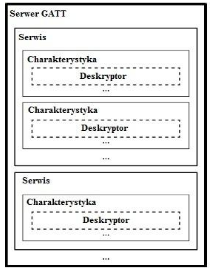
\includegraphics[width=5cm]{img/theory/BLE/ble_services.png}
	\caption{Model struktury danych serwera GATT. Źródło: \cite{inzynierka}}
	\label{fig:image_ble_services}
\end{figure}

Dla charakterystyk zostały zdefiniowane 4 metody komunikacji. Pierwsza z nich - \textit{Write}, polega na wysłaniu danych z urządzenia typu \textit{Central} do \textit{Peripheral}. Druga - \textit{Read}, umożliwia inicjatorowi połączenia odczytanie danych z urządzenia podległego. Pozostałe 2 metody - \textit{Notify} oraz \textit{Indicate} polegają na wysłaniu danych z urządzenia typu \textit{Peripheral} do urządzenia typu \textit{Central} lub odwrotnie, bez żadnego rządania transmisji ze strony odbiorcy. Różnica polega na tym, że \textit{Indicate} wymaga od odbiorcy wysłania potwierdzenia odbioru, a \textit{Notify} nie.



\section{Interfejs NFC}
\label{NFC}

Poniższy rozdział powstał na podstawie źródeł \cite{NFC} i \cite{NFC_NXP}.\\

Near Field Communication to protokół radiowy, stanowiący rozszerzenie swego starszego brata - interfejsu RFID. Mimo, iż jest do niego bardzo podobny w wielu aspektach, różni się znacznie pod względem założeń. RFID (\textit{ang. \textbf{R}adio \textbf{F}requency \textbf{Id}entification}), nie stanowi prawdziwego protokołu komunikacyjnego, bowiem pozwala jedynię na wymianę bardzo krótkich informacji, zwanych identyfikatorami. Urządzenia RFID stanowią bardzo proste układy. Składają się one zazwyczaj z niewielkiego chipa, zawierającego pamięć nieulotną (zazwyczaj do 1 KB) oraz anteny. Przedstawiono to na rysunku \ref{fig:image_rfid_tag}.

\begin{figure}[H]
	\centering
	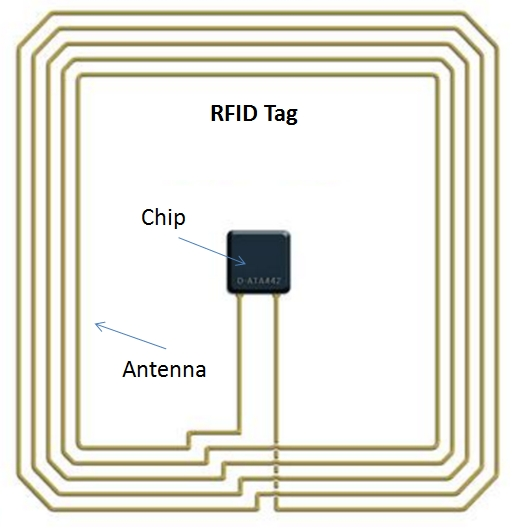
\includegraphics[width=10cm]{img/theory/NFC/RFID_tag.jpg}
	\caption{Budowa tag'a RFID. Źródło: \cite{RFID_antenna}.}
	\label{fig:image_rfid_tag}
\end{figure}

W odróżnieniu od tego, NFC (\textit{ang. \textbf{N}ear \textbf{F}ield \textbf{C}ommunication}) stanowi pełnoprawny protokół komunikacyjny. Umożliwia on wymianę długich wiadomości. Został on zbudowany na podstawie RFID i wykorzystuje jego warstwę fizyczną. Tak samo jak w RFID, w NFC można wyróżnić 2 typy urządzeń - pasywne oraz aktywne. Urządzenie pasywne nie generuje swojego własnego pola elektromagnetycznego, w przeciwieństwie do do urządzenia aktywnego, które inicjuje komunikację. Ponadto, urządzenie bierne, tak samo jak w przypadku RFID nie posiada nawet własnego źródła zasilania. Gdy znajdzie się ono w polu wygenerowanym przez urządzenie aktywne, w jego antenie wyindukuje się prąd, który jest w stanie zasilić niewielki moduł. Komunikacja zwrotna odbywa się poprzez modyfikację zużycia energii tag'a (urządzenia pasywnego) zgodnie z bitowym wzorcem, który należy wysłać. Dynamiczne zmiany parametrów zużycia powodują pewne zaburzenia wygenerowanego przez inicjator pola RF. Odczyt danych przez nie polega na odczycie zmian tego pola. Przedstawiono to na rysunku \ref{fig:image_nfc_comm}. 

\begin{figure}[H]
	\centering
	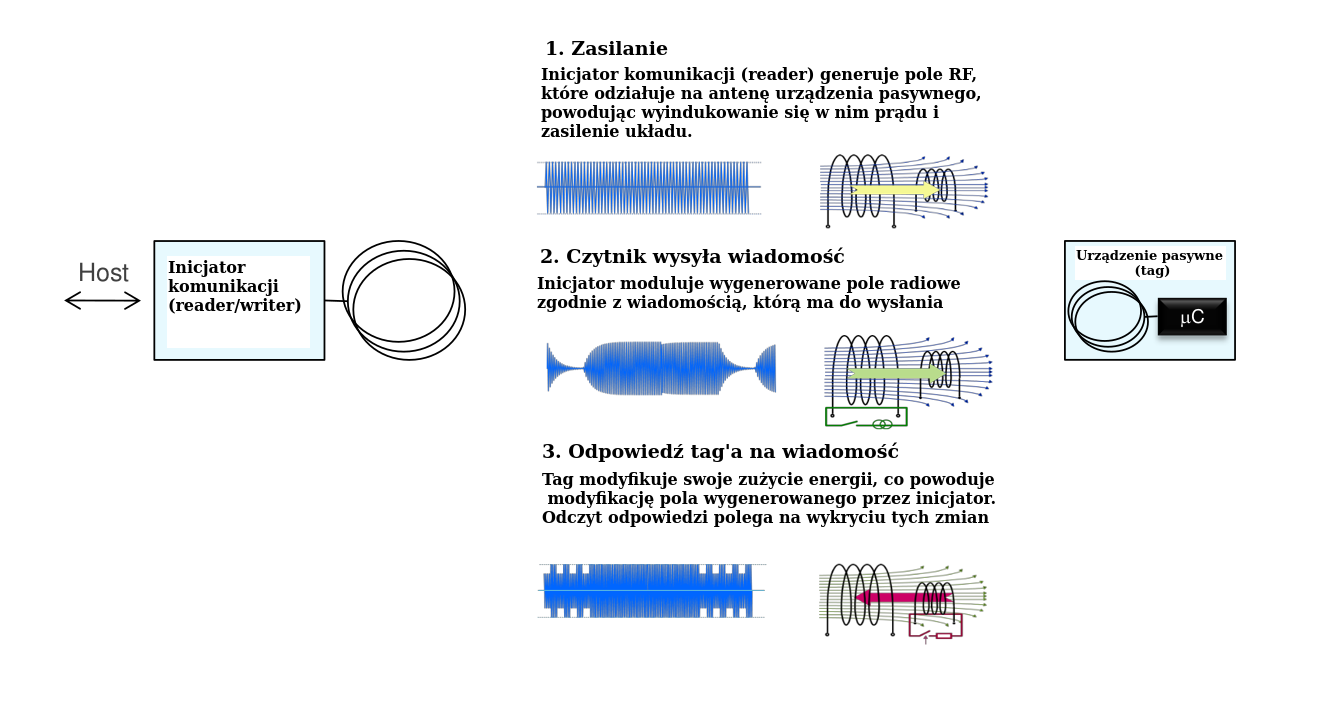
\includegraphics[width=18cm]{img/theory/NFC/NFC_communication.png}
	\caption{Zasada działania komunikacji pomiędzy urządzeniem aktywnym i pasywnym. Źródło: \cite{NFC_NXP}.}
	\label{fig:image_nfc_comm}
\end{figure}

Istnieje również możliwość komunikacji pomiędzy dwoma urządzeniami aktywnymi. Wówczas zamiast modyfikować pole wyindukowane, urządzenie odpowiada swoim własnym, wygenerowanym z energii źródła zasilania. Dzięki temu, możliwy do osiągnięcia zasięg komunikacji jest większy. 

Na tym w zasadzie podobieństwa między NFC i RFID się kończą. RFID pozwala bowiem jedynie na odpowiedź w postaci swojegu unikalnego numeru identyfikacyjnego UID (\textit{ang. \textbf{U}nique \textbf{I}dentifier \textbf{N}umber}), natomiast moduły NFC stanowią najczęściej urządzenia programowalne, pozwalające na przesłanie dowolnej wiadomości. Ponadto, kolejną różnicą jest fakt, że RFID nie posiada jednego wspólnego standardu komunikacji. Co więcej, nie posiada nawet stałej częstotliwości komunikacji, a jej wybór zależy od producenta sprzętu. Zasięg komunikacji w przypadku RFID również jest zmienny i zależny od częstotliwości sygnału. Dla wartości rzędu \linebreak 125 - 134,3 kHz wynosi ona do 30 cm (zazwyczaj około 10 cm), dla częstotliwości \linebreak 13,56 MHz - do 1,5 metra, a w przypadku 433 MHz - nawet do 500 metrów. Ta różnorodność i brak pojedynczego standardu komunikacji stała się główną przyczyną powstania protokołu NFC.

NFC pracuje na ściśle określonej częstotliwości o wartości 13,56 MHz. Zasięg komunikacji jest niewielki (rzędu 10 cm), a urządzenia mają możliwość emulowania tagów RFID, czyli zachowania się jak one gdy wykryte zostanie pole RF. Dodatkowym atutem NFC jest zdefiniowanie formatu komunikacji pomiędzy urządzeniami - NDEF (\textit{ang. \textbf{N}FC \textbf{D}ata \textbf{E}xchange \textbf{F}ormat}). Istnieją pewne dobrze znane struktury danych, możliwe do wysłania poprzez NFC.

 Są to:

\begin{itemize}
\item Wiadomości tekstowe
\item Adresy internetowe URI
\item Proste komendy
\item Podpisy cyfrowe
\end{itemize}

Organizacją zajmującą się standaryzacją i rozwijaniem NFC jest NFC Forum. Definiuje ona 4 rodzaje urządzeń pasywnych:

\begin{enumerate}
	\item Typ 1
	\begin{itemize}
		\item Bazuje na specyfikacji ISO-14443A
		\item Może być tylko do odczytu lub mieć zdolność do zapisu i odczytu
		\item Rozmiar pamięci od 96 B do 2 KB
		\item Prędkość komunikacji - 106 Kb/s
		\item Brak ochrony przed kolizją pól
	\end{itemize}
	
	\item Typ 2
	\begin{itemize}
		\item Bazuje na specyfikacji ISO-14443A
		\item Może być tylko do odczytu lub mieć zdolność do zapisu i odczytu
		\item Rozmiar pamięci od 96 B do 2 KB
		\item Prędkość komunikacji - 106 Kb/s
		\item Zapewnia mechanizm ochrony przed kolizją
	\end{itemize}
	
	\item Typ 3
	\begin{itemize}
		\item Bazuje na specyfikacji ISO-18092 i JS-X-6319-4
		\item Może być tylko do odczytu lub mieć zdolność do zapisu i odczytu
		\item Rozmiar pamięci do 1 MB
		\item Prędkość komunikacji - 212 lub 424 Kb/s
		\item Zapewnia mechanizm ochrony przed kolizją
	\end{itemize}
	\clearpage
	\item Typ 4
	\begin{itemize}
		\item Bazuje na specyfikacji ISO-18092 i JS-X-6319-4
		\item Może być tylko do odczytu lub mieć zdolność do zapisu i odczytu
		\item Rozmiar pamięci: 2, 4 lub 8 KB
		\item Prędkość komunikacji - 106, 212 lub 424 Kb/s
		\item Zapewnia mechanizm ochrony przed kolizją
	\end{itemize}
	
\end{enumerate}




\clearpage
\section{Podsumowanie}

We wcześniejszych podrozdziałach dokonano krótkiej analizy każdego z protokołów i interfejsów wykorzystanych w pracy. Niniejszy podrozdział stanowi ich podsumowanie ze wskazaniem najważniejszych cech, ograniczeń i możliwości wykorzystania. Z rozważań wykluczono jednakże protokół NMEA 0183 ze względu na fakt, iż jest to jedynie narzucony przez producentów modułów GPS standard komunikacji.

\begin{table}[H]
\centering
\caption{Podsumowanie cech systemów i protokołów GSM, GPS, BLE oraz NFC.\\ Źródło: Opracowanie własne.}
\label{table:table_nmea_messages}
\begin{tabular}{| p{2.5cm} | p{3.5cm} | p{3cm} | p{3cm} | p{3.5cm} |}
\hline
\textbf{Parametr} &  \textbf{GSM} & \textbf{GPS}	& \textbf{BLE} & \textbf{NFC} \\ \hline	
\textbf{Właściwości} & - Ogromny zasięg, dzięki rozbudowanej sieci stacji naziemnych & - Zasięg globalny & - Średni zasięg (do 50 m) & - Bardzo bliski zasięg (do 10 cm) \\
			& - Możliwość odbioru i transmisji & - Tylko do odczytu & - Możliwość odbioru i transmisji & - Możliwość odbioru i transmisji \\
			& - Prędkość rzędu 57.6 kb/s (odbiór) i 14.5 kb/s (transmisja) & - 50 bit/s & - Około 125 kb/s & - Około 106 kb/s \\
			& - Wysoki pobór pradu (w szczycie do 1.5 A) & - Średni pobór prądu (ok. 30 mA w trakcie śledzenia pozycji) & - Niski pobór prądu (ok. 7 - 14 mA nateżęnia chwilowego w trakcie transmisji) & - Pobór energii rzędu 100 mA w trybie inicjatora, 0 mA w trybie pasywnym \\ \hline
\textbf{Możliwości wykorzystania} & - Rozmowy głosowe & - Odczyt lokalizacji & - Energooszczędna transmisja danych & - Bezpieczna, bezkontaktowa transmisja danych \\
						& - Wiadomości SMS & - Bardzo dokładny odczyt prędkości & & - Parowanie urządzeń \\
						& - Dostęp do internetu & - Bardzo dokładne źródło czasu & & - Wymiana kluczy szyfrujących \\ \hline
\end{tabular}
\end{table}


%\clearpage{\pagestyle{empty}\cleardoublepage}

\chapter{Schematy elektroniczne urządzeń}
\label{schematics}

\section{Urządzenie lokalizujące}
Ze względu na poziom skomplikowania układu, schemat elektroniczny musiał zostać rozbity na podschematy. W urządzeniu lokalizującym można wyróżnić trzy znaczące moduły elektroniczne, realizujące odpowiednie funkcje. Są to:

\begin{itemize}
\item Moduł zasilania, przedstawiony na rysunku \ref{fig:image_mainboard_power_schematic}
\item Moduł funkcjonalny, przedstawiony na rysunku \ref{fig:image_mainboard_functional_schematic}
\item Moduł NFC, przedstawiony na rysunku \ref{fig:image_mainboard_NFC_schematic}
\end{itemize}

\begin{figure}[H]
	\centering
	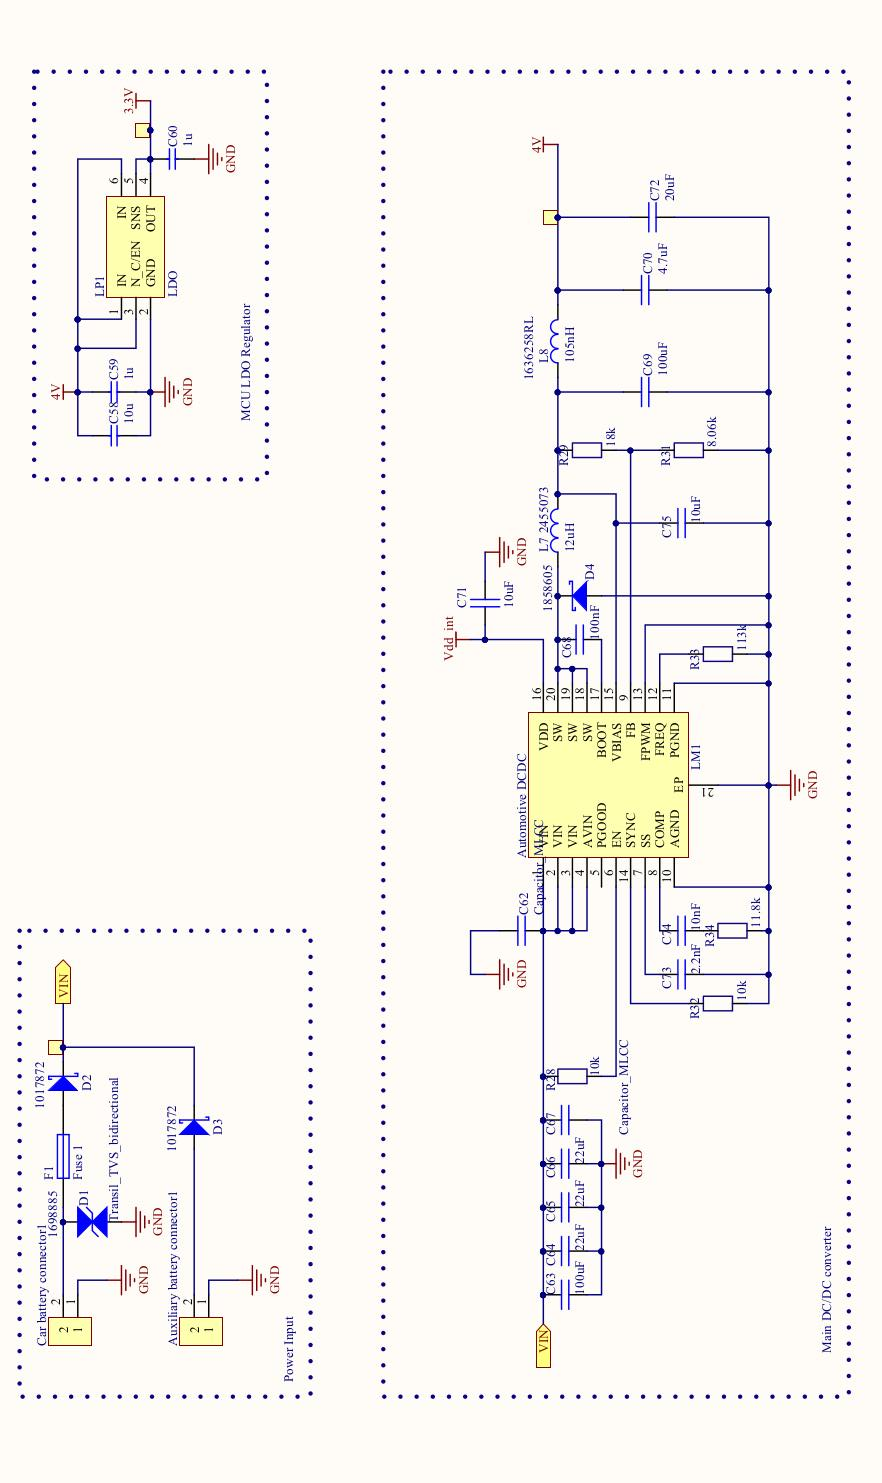
\includegraphics[width=14cm]{img/schematics/mainboard_power.jpg}
	\caption{Schemat modułu zasilania urządzenia lokalizującego. \\ Źródło: Twórczość własna}
	\label{fig:image_mainboard_power_schematic}
\end{figure}

\begin{figure}[H]
	\centering
	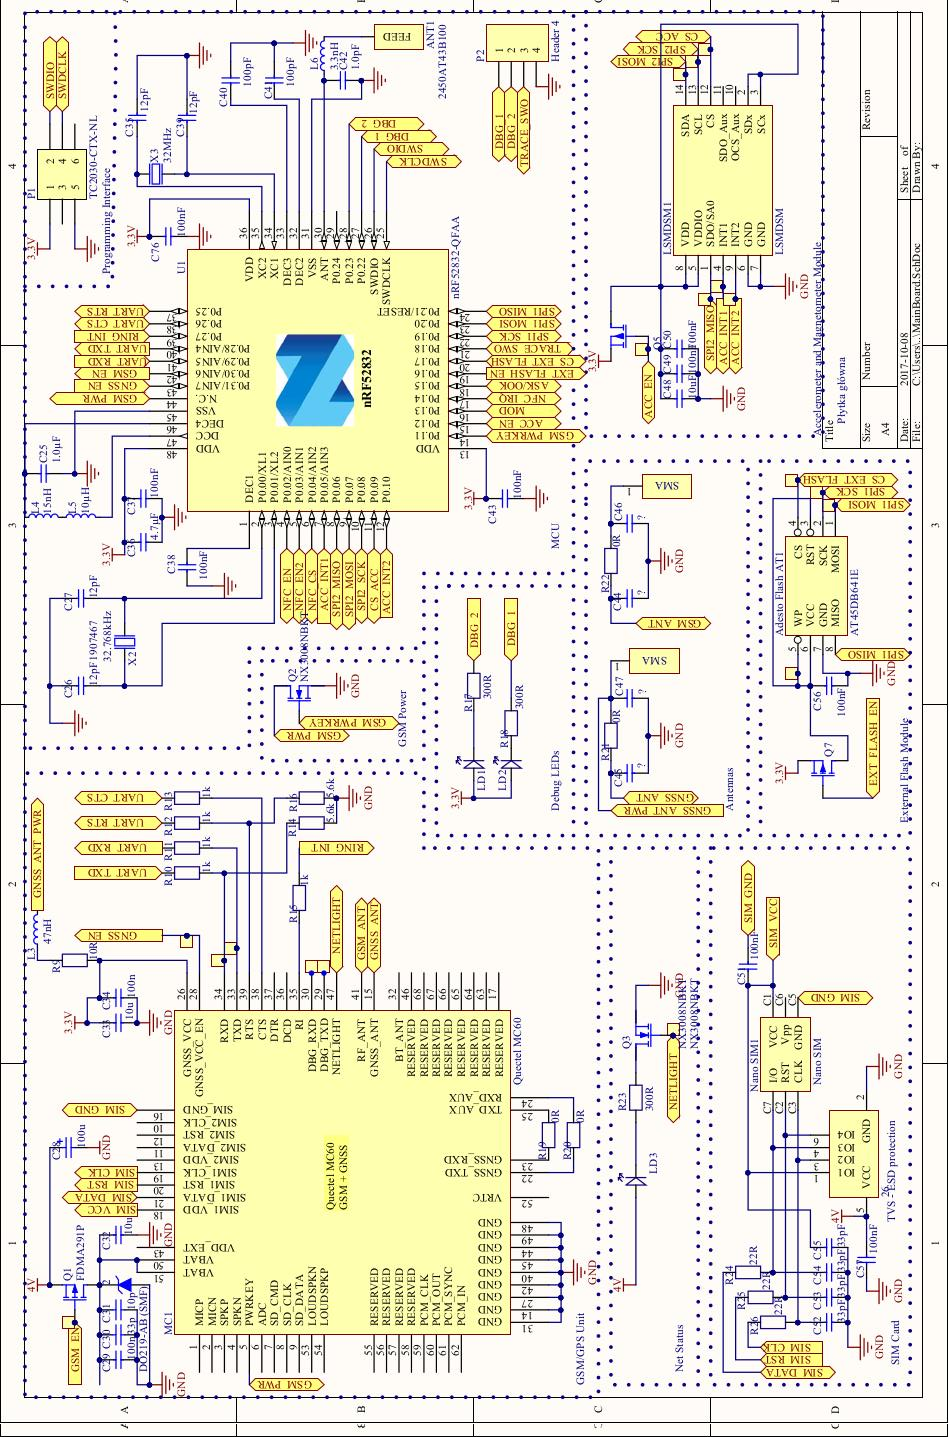
\includegraphics[width=14cm]{img/schematics/mainboard_functional.jpg}
	\caption{Schemat modułu funkcjonalnego urządzenia lokalizującego. \\ Źródło: Twórczość własna}
	\label{fig:image_mainboard_functional_schematic}
\end{figure}

\begin{figure}[H]
	\centering
	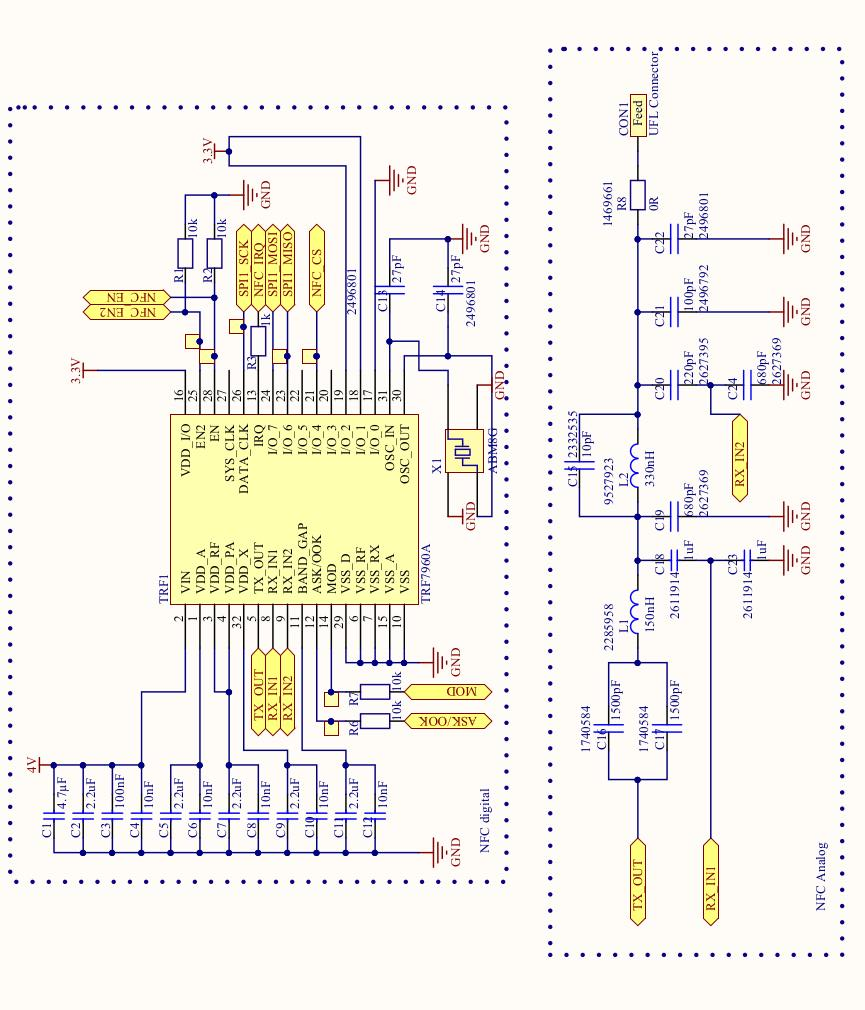
\includegraphics[width=14cm]{img/schematics/mainboard_NFC.jpg}
	\caption{Schemat modułu NFC urządzenia lokalizującego. \\ Źródło: Twórczość własna}
	\label{fig:image_mainboard_NFC_schematic}
\end{figure}



\subsection{Schemat zasilania}

Akumulator samochodowy jest bardzo wygodnym źródłem zasilania układów elektronicznych, lecz gdy są one niewłaściwie zaprojektowane, bywa on dla nich zabójczy. Bliska odległość do alternatora i innych urządzeń indukcyjnych powoduje generowanie silnych zakłóceń na linii zasilającej. Niekiedy "szpilki" napięciowe osiągają wartość rzędu 100V. Z tego powodu należy stosować transile – diody zabezpieczające. Powodują one ograniczenie zbyt dużego napięcia do pewnej maksymalnej wartości. W przypadku zastosowanego przeze mnie komponentu wynosi ono 24.4V. Zabezpieczenie przeciążeniowe stanowi bezpiecznik samochodowy o wartości 4A. 
Ponieważ jednym z wymagań układu jest możliwość zasilania bateryjnego, konieczne jest zastosowanie dodatkowego przyłącza zasilania. Urządzenie można zasilić dowolną baterią o napięciu od 4 do 38V i wydajności prądowej co najmniej 3A w szczycie. Ze względu na prawdopodobieństwo wystąpienia różnic napięć pomiędzy dodatkową baterią, a akumulatorem samochodu i wiążącym się z tym przepływem prądu z jednego źródła do drugiego, konieczne jest zastosowanie diód zabezpieczających przed rozładowaniem baterii przez akumulator (gdy napięcie akumulatora niższe niż napięcie baterii) lub mogącym doprowadzić baterię do zniszczenia doładowywaniem jej bezpośrednio z akumulatora (gdy napięcie baterii jest od niższe napięcia akumulatora). W trakcie projektowania, zdecydowano się na zastosowanie diód Schottky’ego ze względu na ich niski spadek napięcia (0.2 - 0.55V w zależności od natężenia prądu) oraz szybki czas przełączania ze stanu zaporowego do przewodzenia (ograniczenie krótkotrwałych zaników zasilania przy wyłączaniu samochodu). Na rysunku \ref{fig:image_mainboard_power_input} przedstawiono część wejściową dla zasilania całej płytki.

\begin{figure}[H]
	\centering
	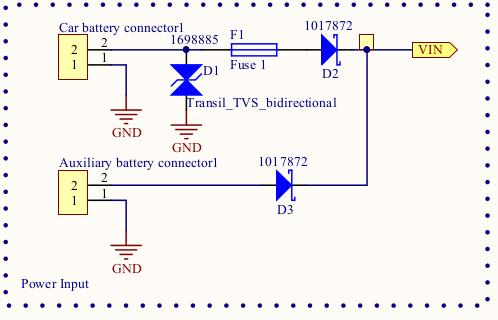
\includegraphics[width=10cm]{img/schematics/mainboard_power_input.jpg}
	\caption{Schemat modułu zasilania wejściowego urządzenia lokalizującego. \\ Źródło: Twórczość własna}
	\label{fig:image_mainboard_power_input}
\end{figure}

Niestety, często napięcie wejściowe, nawet po zadziałaniu zabezpieczenia w postaci transila, jest nadal zbyt duże dla zwykłych układów zasilających. Stąd konieczne jest stosowanie przetwornic impulsowych klasy automotive, które umożliwiają zasilanie napięciem wejściowym do kilkudziesięciu woltów. Schemat wykorzystanej przetwornicy przedstawiono na rysunku \ref{fig:image_mainboard_power_converter}.

\begin{figure}[H]
	\centering
	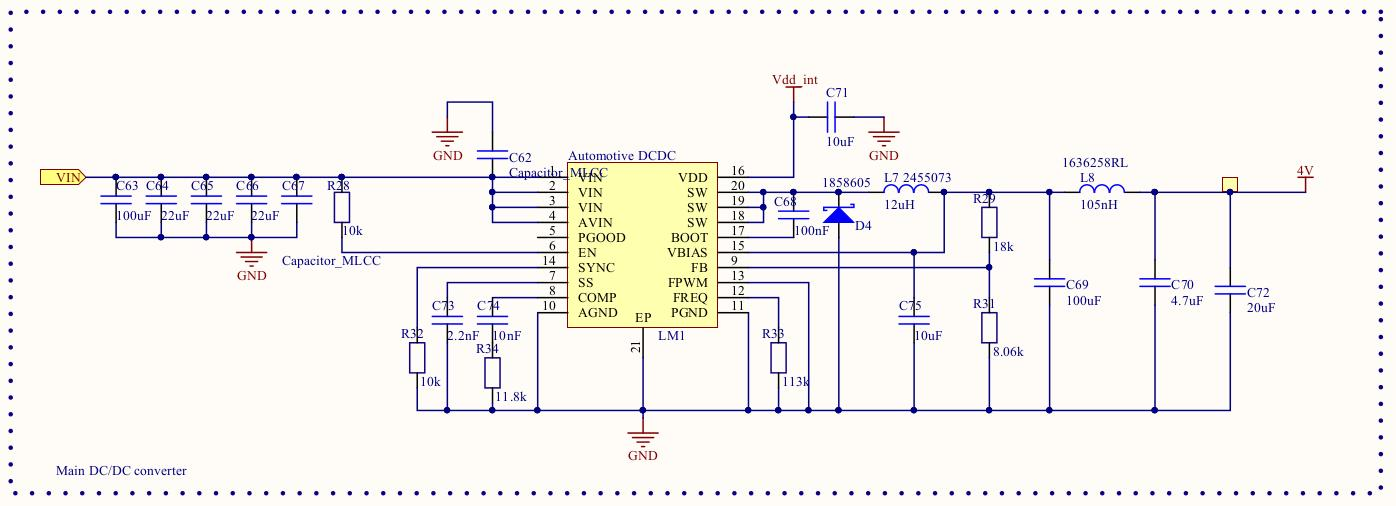
\includegraphics[width=17cm]{img/schematics/mainboard_power_converter.jpg}
	\caption{Schemat przetwornicy impulsowej modułu zasilania urządzenia lokalizującego. \\ Źródło: Twórczość własna}
	\label{fig:image_mainboard_power_converter}
\end{figure}

Zastosowana w urządzeniu przetwornica umożliwia zasilanie napięciami od 4 do 38V. Wybrano ją ze względu na niewielką liczbę zewnętrznych komponentów, niezbędnych do jej działania w porównaniu do innych modułów, a także wysoką sprawność rzędu od 85\% do 90\% w zależności od chwilowego natężenia prądu. Wytwarza ona na wyjściu napięcie o wartości 4V, którym zasilany jest moduł GSM oraz dalszy stopień obniżania napięcia.

Ostatni stopień zasilania generuje z napięcia wyjściowego z przetwornicy napięcie o wartości 3.3V. Jest ono niezbędne do zasilania układów mikrokontrolera, pamięci flash, akcelerometru oraz układu GPS. Szacowany pobór prądu przez te układy wynosi ok. 200mA w szczycie, stąd dla bezpieczeństwa wykorzystano stabilizator napięcia LDO (ang. Low Dropout Stabilizer) o maksymalnym natężeniu wyjściowym 0,5A. Jego schemat przdstawiono na rysunku \ref{fig:image_mainboard_power_ldo}.

\begin{figure}[H]
	\centering
	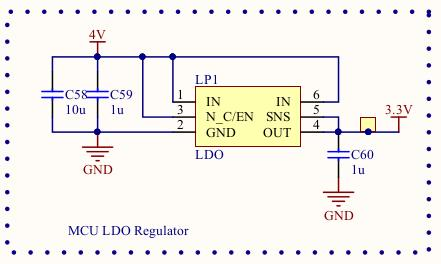
\includegraphics[width=12cm]{img/schematics/mainboard_power_ldo.jpg}
	\caption{Schemat stabilizatora napięcia modułu zasilania urządzenia lokalizującego. \\ Źródło: Twórczość własna}
	\label{fig:image_mainboard_power_ldo}
\end{figure}

\subsection{Moduł mikrokontrolera}

Serce urządzenia stanowi mikrokontroler nRF52832 firmy Nordic Semiconductor. Układ ten posiada 32 bitowy rdzeń Cortex-M4 zaprojektowany przez firmę ARM, sprzętową jednostkę FPU, 512kB wewnętrznej pamięci Flash oraz 64kB pamięci RAM. Zdecydowano się na wykorzystanie tego mikrokontrolera ze względu na kilka czynników. Pierwszym z nich jest jego wyposażenie - posiada wbudowany układ radiowy działający na częstotliwości 2.4 GHz i umożliwiający komunikację w standardzie Bluetooth Low Energy, ANT lub wykorzystanie własnego protokołu. Dodatkowym atutem tego mikrokontrolera jest wyposażenie w sprzętowy interfejs NFCT, umożliwiający wykorzystanie modułu jako tag (urządzenie podrzędne) w komunikacji poprzez interfejs NFC. Ponadto ma bardzo duże możliwości obliczeniowe – wewnętrzny zegar 64 MHz umożliwia bardzo szybkie wykonywanie zaprogramowanych zadań i szybki powrót do trybu oszczędzania energii. Zużycie energii przez ten procesor jest bardzo niewielkie. W trakcie wykonywania programu pobór prądu wynosi 58 $\mu A$ /MHz gdy kod wykonywany jest z pamięci flash, natomiast w trybie oszczędzania energii pobór spada do ok 1.9 $\mu A$. Ostatnim i być może najważniejszym czynnikiem decydującym na wybranie tego układu jest posiadane przez autora doświadczenie zawodowe w programowaniu układów od tego producenta, a zatem bardzo dobra znajomość jego możliwości i SDK (\textit{ang. \textbf{S}oftware \textbf{D}evelopment \textbf{K}it}). Schemat mikrokontrolera przedstawiono na rysunku \ref{fig:image_mainboard_functional_mcu}.

\begin{figure}[H]
	\centering
	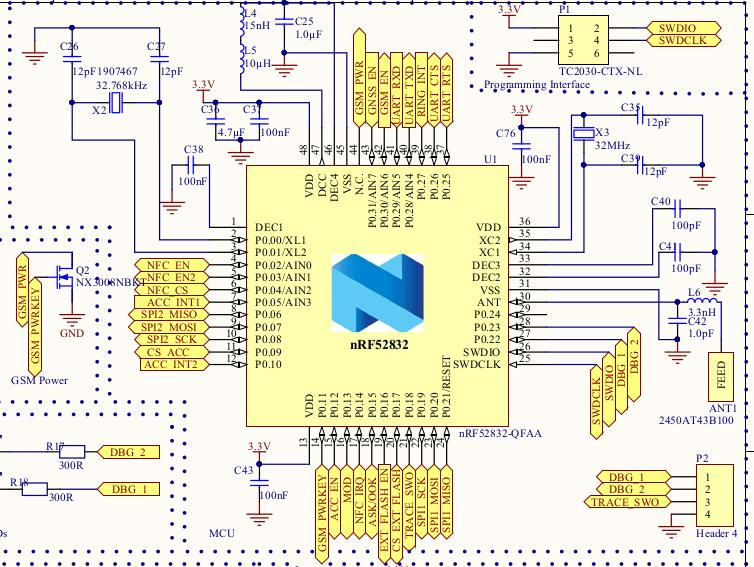
\includegraphics[width=15cm]{img/schematics/mainboard_functional_mcu.jpg}
	\caption{Schemat modułu mikrokontrolera w urządzeniu lokalizującym. \\ Źródło: Twórczość własna}
	\label{fig:image_mainboard_functional_mcu}
\end{figure}

\subsection{Moduł GSM i GPS}

Jako moduł realizujący główną funkcję urządzenia wybrano układ Quectel MC60. Stanowi on połączenie modułu GSM oraz GPS w jednym chipie. Umożliwia transmisję w wielu protokołach, takich jak: TCP/IP, UDP, FTP, PPP, HTTP czy NTP. Ponadto możliwe jest odbieranie i wysyłanie danych w postaci krótkich wiadomości SMS. Układ posiada niewielkie wymiary: 18.7 mm x 16 mm x 2.1 mm dzięki czemu możliwe będzie zmniejszenie całego urządzenia. Zużycie energii wynosi:
\begin{itemize}
\item Około 25 mA gdy działa jedynie moduł GPS
\item Do 1.6 A w trakcie transmisji danych poprzez sieć GSM
\end{itemize}

Ponadto, kombinacja tych dwóch systemów umożliwia wykorzystanie funkcjonalności AGPS. Polega ona na podaniu do modułu GPS zgrubnych danych o położeniu satelitów, pobranych z sieci GSM. Dzięki temu, ustalenie własnej lokalizacji, nawet po długotrwałym wyłączeniu, trwa ok. sekundy (tzw. warm start). Schemat modułu GSM i GPS przedstawiono na rysunku \ref{fig:image_mainboard_functional_gps_gsm}.

\begin{figure}[H]
	\centering
	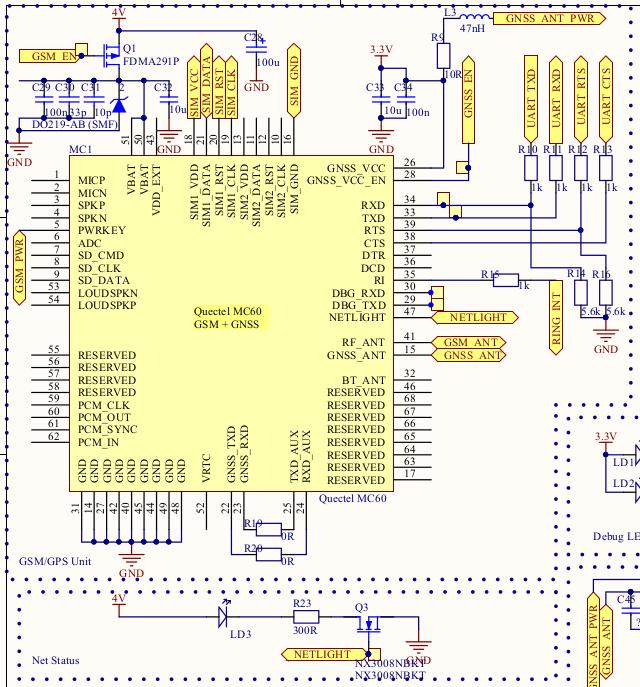
\includegraphics[width=15cm]{img/schematics/mainboard_functional_gps.jpg}
	\caption{Schemat modułu układu GSM i GPS w urządzeniu lokalizującym. \\ Źródło: Twórczość własna}
	\label{fig:image_mainboard_functional_gps_gsm}
\end{figure}

W celu zwiększenia niezawodności działania urządzenia, zdecydowano zastosować zewnętrzne anteny GSM i GPS poprawiające jakość sygnału. Dodatkowo, w celu dalszej jego poprawy, antena GPS jest anteną aktywną. Oznacza to, że dostarczane jest do niej dodatkowe zasilanie, co powoduje wzmocnienie odebranego sygnału. Schemat anten przedstawiono na rysunku \ref{fig:image_mainboard_functional_gps_gsm_antennas}. Zawarte na nim znaki zapytania, zamiast wartości kondensatorów oznaczają, że kondensatory należy dobrać po złożeniu płytki i przebadaniu jej pod kątem jak najlepszego dopasowania impedancji.

\begin{figure}[H]
	\centering
	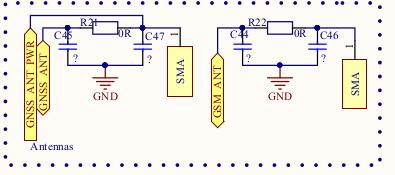
\includegraphics[width=15cm]{img/schematics/mainboard_functional_gps_gsm_antennas.jpg}
	\caption{Schemat modułu anten dla GSM i GPS w urządzeniu lokalizującym. \\ Źródło: Twórczość własna}
	\label{fig:image_mainboard_functional_gps_gsm_antennas}
\end{figure}

Ostatnią częścią układu GSM jest połączenie modułu z kartą SIM, umożliwiającą zalogowanie do sieci. Przedstawiono je na rysunku \ref{fig:image_mainboard_functional_gsm_sim_card}. Widać na nim układ TVS, który jest odpowiedzialny za zabezpieczenie wrażliwej elektroniki w karcie SIM przed wyładowaniami statycznymi ESD (\textit{ang. \textbf{E}lectro\textbf{s}tatic \textbf{d}ischarge}).

\begin{figure}[H]
	\centering
	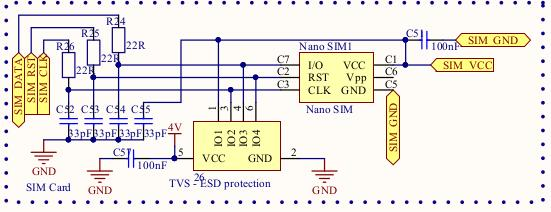
\includegraphics[width=15cm]{img/schematics/mainboard_gsm_sim_card.jpg}
	\caption{Schemat modułu karty SIM w urządzeniu lokalizującym. \\ Źródło: Twórczość własna}
	\label{fig:image_mainboard_functional_gsm_sim_card}
\end{figure}

\subsection{Moduł pamięci flash}

Wewnętrzna pamięć flash mikrokontrolera jest niewystarczająca, aby przechowywać w niej trasy wraz z parametrami jazdy. Stąd też pojawia się konieczność zastosowania zewnętrznego układu pamięci nieulotnej. Zastosowana w urządzeniu pamięć flash posiada pojemność 8 MB, co umożliwi przechowywanie wielu długich tras oraz dokładne profilowanie statystyczne stylu jazdy kierowcy. Schemat podłączenia pamięci w urządzeniu lokalizującym pokazano na rysunku \ref{fig:image_mainboard_functional_flash}.

\begin{figure}[H]
	\centering
	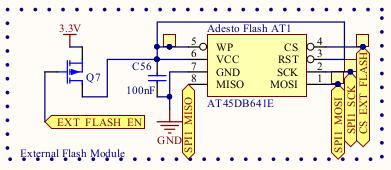
\includegraphics[width=15cm]{img/schematics/mainboard_functional_flash_memory.jpg}
	\caption{Schemat modułu pamięci flash w urządzeniu lokalizującym. \\ Źródło: Twórczość własna}
	\label{fig:image_mainboard_functional_flash}
\end{figure}

\subsection{Moduł akcelerometru}

Kolejną ważną częścią urządzenia jest moduł akcelerometru. Pozwala on na wybudzenie urządzenia w momencie przemieszczenia pojazdu, a w razie braku dezaktywacji - uruchomienie procedury alarmowej. Ponadto, dzięki jego wskazaniom możliwe jest wyznaczenie przyspieszenia pojazdu pozwalające na profilowanie stylu prowadzenia pojazdu przez kierowcę. Wbudowany żyroskop pozwoli na dokładniejsze profilowanie stylu jazdy kierowcy w trakcie pokonywania zakrętów oraz zmiany pasa.
Schemat modułu akcelerometru przedstawiono na rysunku \ref{fig:image_mainboard_functional_accelerometer}.

\begin{figure}[H]
	\centering
	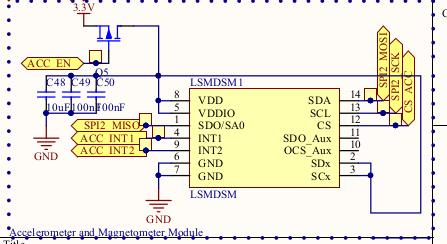
\includegraphics[width=15cm]{img/schematics/mainboard_functional_accelerometer.jpg}
	\caption{Schemat modułu akcelerometru w urządzeniu lokalizującym. \\ Źródło: Twórczość własna}
	\label{fig:image_mainboard_functional_accelerometer}
\end{figure}

\subsection{Moduł NFC}

Moduł ten stanowi istotną część z punktu widzenia bezpieczeństwa komunikacji bezprzewodowej. Jest ono zapewnione poprzez zastosowanie szyfrowania wiadomości. Jeśli jednak ktoś podsłucha transmisję inicjalizacji urządzenia, w której przekazywane są klucze szyfrujące, cały koncept traci sens. Dzięki zastosowaniu modułu NFC, możliwość podsłuchania transmisji wymiany kluczy szyfrujących zostaje zniwelowana poprzez fizyczne ograniczenia zasięgu komunikacji. NFC posiada zasięg maksymalny do 10 cm.
Komunikacja odbywa się pomiędzy dwoma urządzeniami. Ze względu na sposób transmisji, jedno z urządzeń inicjuje komunikację. Inicjator generuje zmienne pole magnetyczne, w którym może (lecz nie musi) zawrzeć dane wysyłane do urządzenia docelowego. Urządzenie docelowe wykrywa to pole i może odpowiedzieć poprzez odpowiednie zniekształcenie go, które jest wykrywane przez inicjator. Urządzenie docelowe nie generuje żadnego pola magnetycznego. Może jedynie zniekształcać pole generowane przez inicjator. Stąd wynika, że inicjator musi mieć znacznie większe zużycie energii niż urządzenie docelowe – tag. W urządzeniu lokalizacyjnym zastosowano moduł inicjatora NFC, którego schemat przedstawiono na rysunkach \ref{fig:image_mainboard_NFC_digital} - część cyfrowa oraz \ref{fig:image_mainboard_NFC_analog} - część analogowa.

\begin{figure}[H]
	\centering
	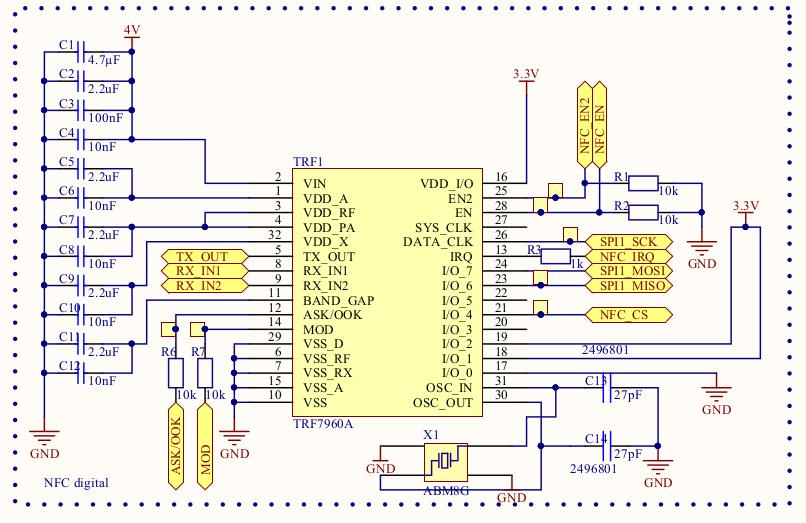
\includegraphics[width=15cm]{img/schematics/mainboard_NFC_chip.jpg}
	\caption{Schemat części cyfrowej modułu NFC w urządzeniu lokalizującym. \\ Źródło: Twórczość własna}
	\label{fig:image_mainboard_NFC_digital}
\end{figure}

\begin{figure}[H]
	\centering
	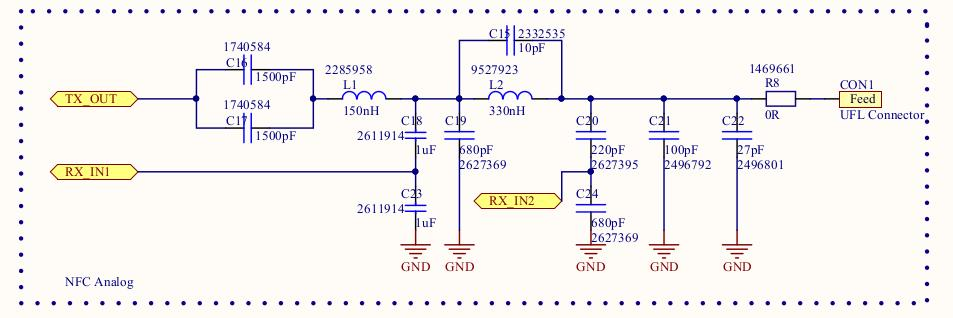
\includegraphics[width=15cm]{img/schematics/mainboard_NFC_analog.jpg}
	\caption{Schemat części analogowej modułu NFC w urządzeniu lokalizującym. \\ Źródło: Twórczość własna}
	\label{fig:image_mainboard_NFC_analog}
\end{figure}


\clearpage
\section{Urządzenie deaktywujące}

Głównym zadaniem tego urządzenia jest cykliczne rozgłaszanie swej obecności. Po wykryciu przez urządzenie lokalizujące, łączy się ono z deaktywatorem oraz bezpiecznym kanałem dokonywane jest wyłączenie funkcji alarmu. Dzięki temu, że urządzenie to ma tak proste zadanie, nie pobiera ona dużo    energii, więc możliwe jest zasilenie go ze standardowej baterii CR2032 o promieniu 20 mm i grubości 3.2 mm. Urządzenie to, przy odpowiedniej konfiguracji parametrów transmisji może działać kilka lat bez konieczności jej wymiany. Zastosowanie wspomnianego źródła zasilania stanowi kompromis pomiędzy czasem działania i rozmiarem urządzenia, które docelowo powinno być umieszczone przy kluczach samochodowych. Schemat deaktywatora przedstawiono na rysunku \ref{fig:image_mainboard_NFC_schematic}.

\begin{figure}[h]
	\centering
	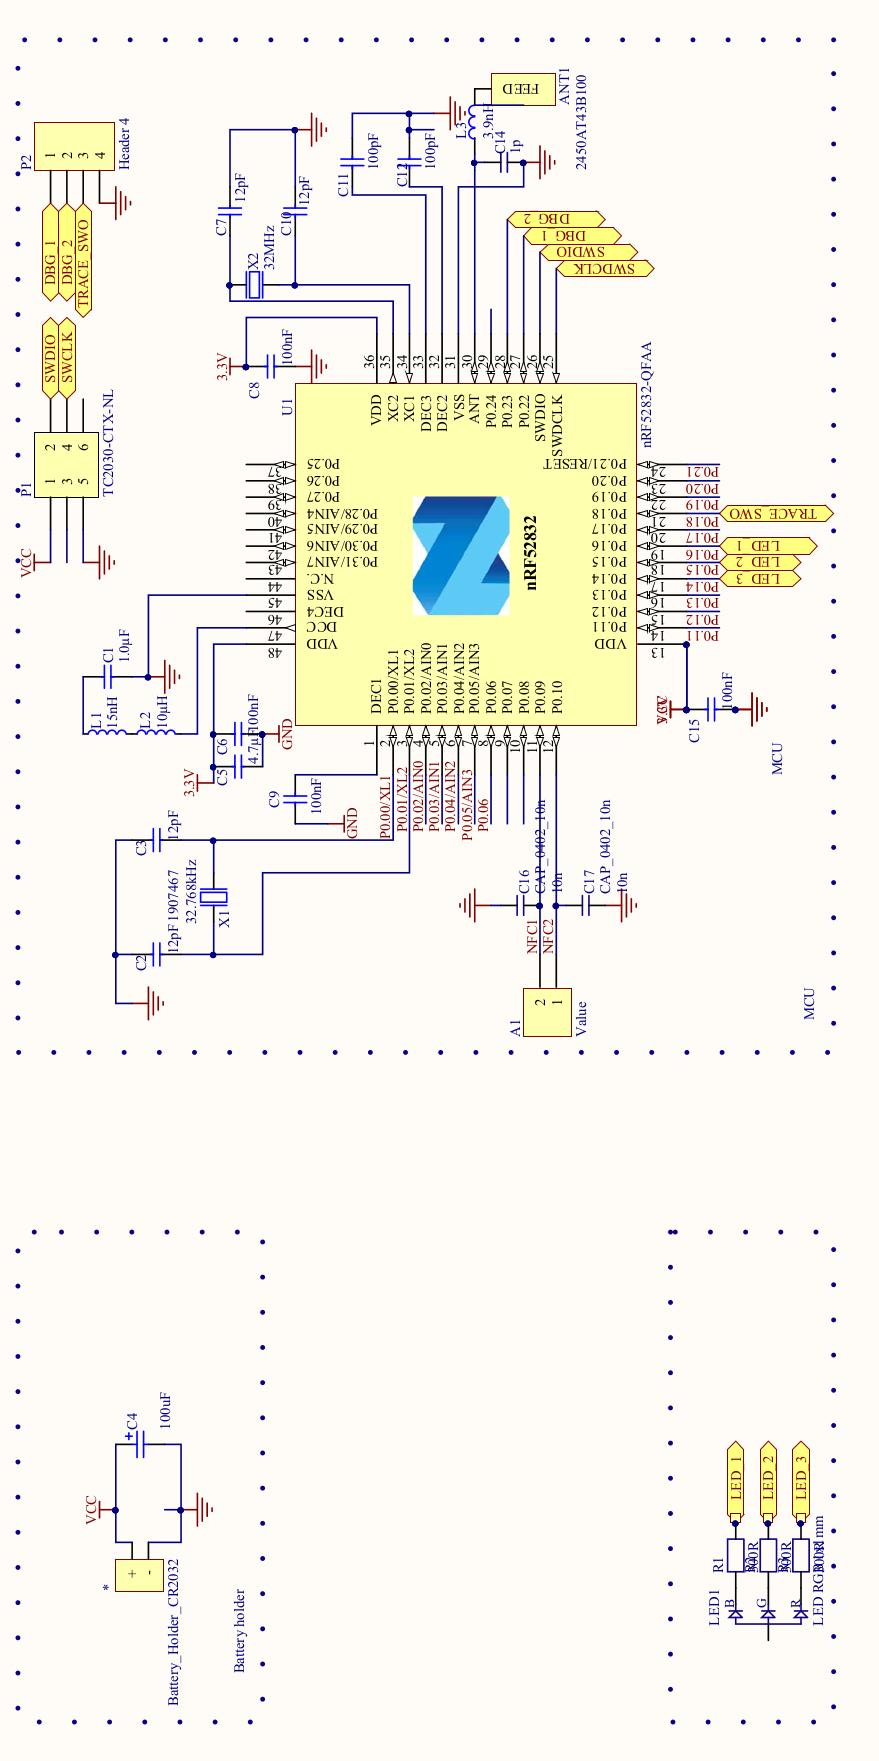
\includegraphics[width=12cm]{img/schematics/keytag.jpg}
	\caption{Schemat modułu zasilania urządzenia deaktywującego. \\ Źródło: Twórczość własna}
	\label{fig:image_keytag_schematic}
\end{figure}

%\clearpage{\pagestyle{empty}\cleardoublepage}

\chapter{Schematy płytek drukowanych}
\label{boards}

\section{Urządzenie deaktywujące}

Ze względu na pełniony przez urządzenie cel, powinno ono zawsze towarzyszyć osobie upoważnionej do uruchomienia pojazdu. Biorąc pod uwagę przykład zastosowania urządzenia we flotach pojazdów, szybko można zauważyć, że zazwyczaj do pojazdu nie jest przypisana jedna osoba, lecz może być on używany przez wielu kierowców. Stąd też logicznym staje się wniosek, że urządzenie nie może być przyporządkowane do kierowcy, lecz do pojazdu. Idealnym rozwiązaniem wydaje się umieszczenie go przy kluczykach lub karcie umożliwiającej uruchomienie pojazdu bezkluczykowo, jako dodatkowy brelok. Z tego powodu ważne stają się wymiary samego urządzenia. Nie powinno być ono zbyt grube, aby nie przeszkadzało w kieszeni, ani zbyt duże, aby nie obijało się o nogi, a tym samym nie rozpraszało kierującego w trakcie jazdy.
Rozmiar płytki urządzenia dezaktywującego wynoszą odpowiednio 32 mm x 43 mm szerokości i wysokości.

Ze względu na prostotę urządzenia, składa się ono z bardzo niewielu modułów.
Na górnej warstwie płytki znajduje się serce układu - mikrokontroler nRF52832 wraz z anteną 2.4 GHz ISM do komunikacji poprzez Bluetooth Low Energy. Dodatkowo, znajdują się tam złącze do programowania, złącze debugowe oraz antena NFC, zwizualizowana jako koło w kolorze niebieskim. Górną warstwę płytki przedstawiono na rysunku \ref{fig:image_key_tag_top_board}.

Centralne miejsce na dolnej warstwie płytki zajmuje bateria litowa CR2032, która zapewni kilkuletnią pracę dezaktywatora. Posiada ona średnicę 20mm oraz grubość 3.2 mm co stanowi idealny kompromis pomiędzy wymiarami urządzenia, a czasem jego pracy, bowiem mniejsze baterie oferują mniejszą pojemność liczoną w miliampero godzinach. Wygląd oraz wizualizację dolnej warstwy płytki przedstawiono na rysunku \ref{fig:image_key_tag_bottom_board}.

\begin{figure}[H]
\centering
	\subfloat[Wygląd górnej warstwy płytki]{
		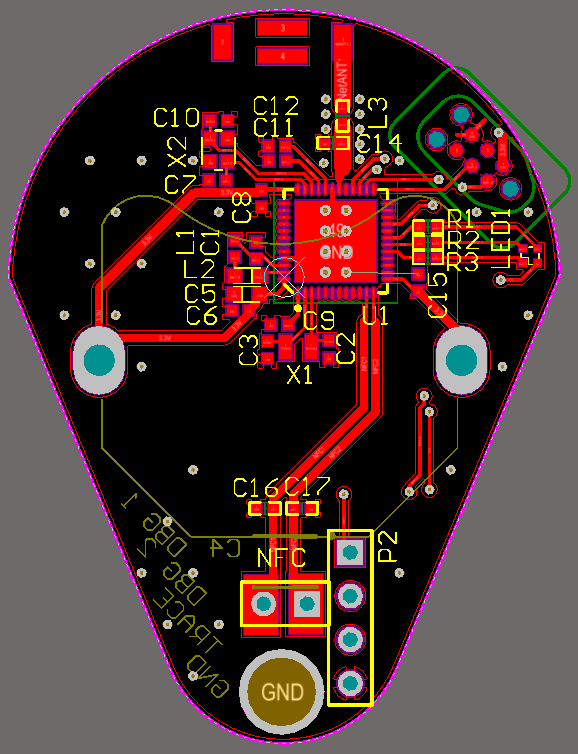
\includegraphics[width=6cm]{img/board_layouts/key_tag_top.png}
	}
	\qquad
	\subfloat[Wizualizacja górnej warstwy płytki]{
		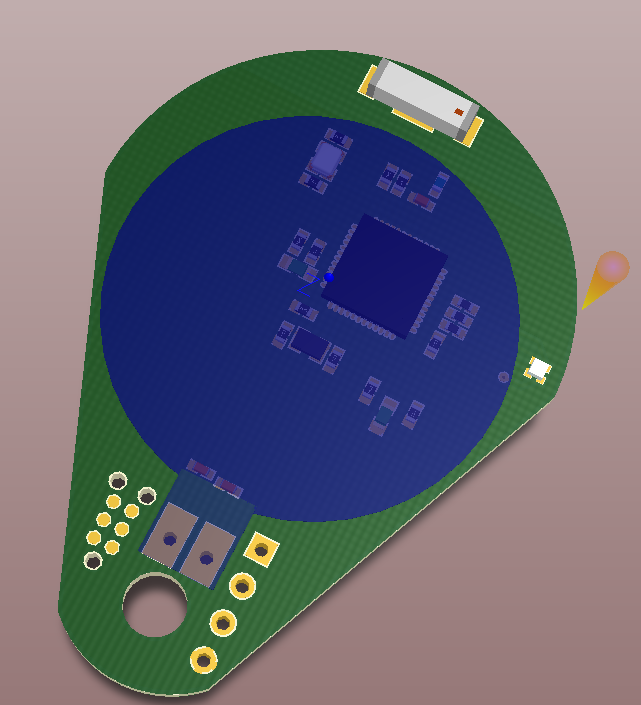
\includegraphics[width=7.1cm]{img/board_layouts/key_tag_visualization_top.png}
	}
	
	\caption{Wygląd górnej warstwy płytki urządzenia dezaktywującego oraz jej wizualizacja. \\ Źródło: Twórczość własna}
	\label{fig:image_key_tag_top_board}
\end{figure}

\begin{figure}[H]
\centering
	\subfloat[Wygląd dolnej warstwy płytki]
	{
		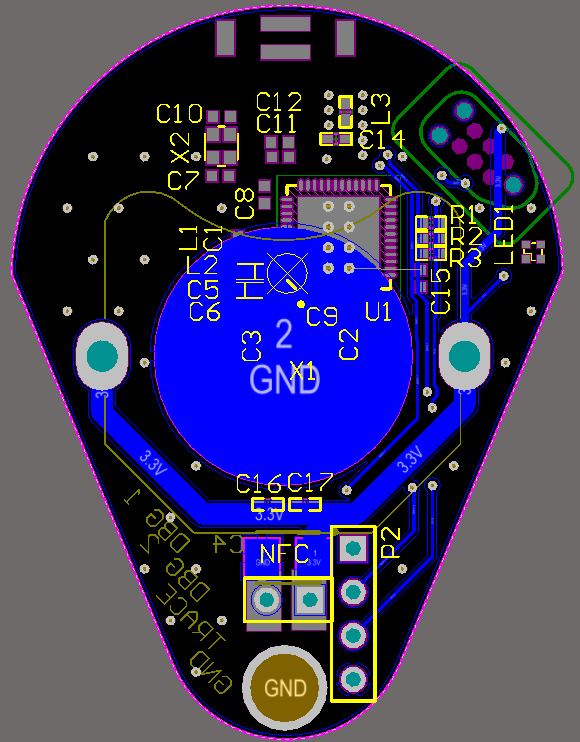
\includegraphics[width=6cm]{img/board_layouts/key_tag_bottom.png}
	}
	\qquad
	\subfloat[Wizualizacja dolnej warstwy płytki]
	{
		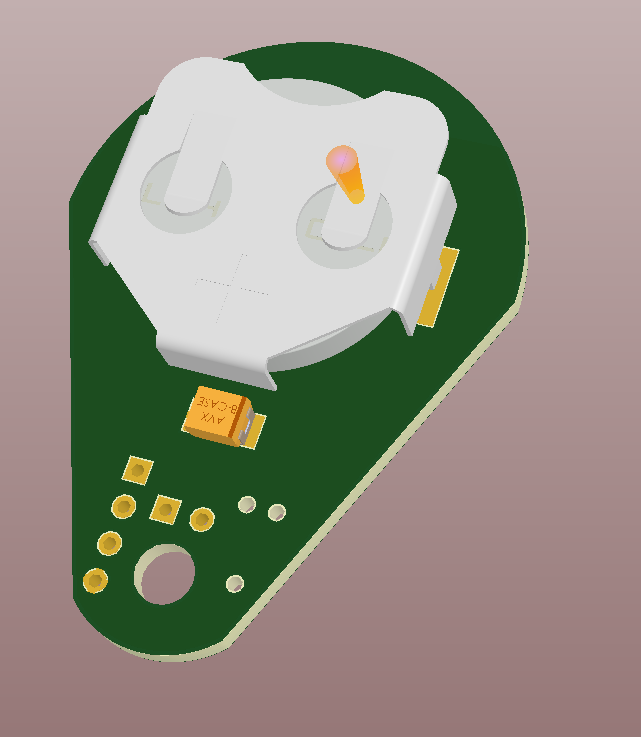
\includegraphics[width=7.1cm]{img/board_layouts/key_tag_visualization_bottom.png}
	}
	
	\caption{Wygląd dolnej warstwy płytki urządzenia dezaktywującego oraz jej wizualizacja. \\ Źródło: Twórczość własna}
	\label{fig:image_key_tag_bottom_board}
\end{figure}

\section{Urządzenie lokalizujące}

Płytka lokalizująca jest znacznie bardziej skomplikowana od urządzenia dezaktywującego. Wynika to głównie z faktu, iż stanowi podstawę funkcjonalności całego systemu, a zatem posiada wiele modułów realizujących określone zadania. Płytka ma wymiary 50 mm x 50 mm, co powinno umożliwić ukrycie jej w większości miejsc w pojeździe (na przykład pod plastikowymi zabudowami kokpitu). 

Wygląd i wizualizacje urządzenia przedstawiono na rysunkach \ref{fig:image_mainboard_top_board} oraz \ref{fig:image_mainboard_bottom_board}.

Ze względu na użycie kilku układów radiowych, wykorzystujących częstotliwości od 13.56 MHz (NFC), poprzez 900 MHz/ 1800 MHz (GSM) i 1575.42 MHz (GPS) aż po 2.4 GHz (Bluetooth), a także przetwornicy impulsowej o znacznym szczytowym natężeniu prądu (aż do 2.5 A), niezbędne jest odpowiednie rozłożenie elmentów na płytce, które zminimalizowałoby ich wzajemny wpływ. W związku z tym, postanowiono umieścić kluczowe elementy zasilające oraz radiowe w rogach płytki, aby zmaksymalizować wzajemne odległości. W ten sposób, w lewym górnym rogu płytki umieszczono złącza zasilania wejściowego, w prawym górnym - cewkę indukcyjną, stanowiącą główny element impulsowej stabilizacji napięcia. Cewka ta przy okazji stanowi główne źródło zakłóceń sygnałów. W lewym dolnym rogu znajduje się antena Bluetooth Low Energy, natomiast w prawym dolnym rogu - złącze anteny GPS. 

Przewody anten GPS oraz GSM są dodatkowo ekranowane, dzięki czemu znacznie zmniejszona jest podatność tych sygnałów na zakłócenia w trakcie przepływu od anteny do płytki. Jednakże na samej płytce sygnały te nie posiadają ekranu elektromagnetycznego, przez co są podatne na szumy. Z tego względu niezbędna jest minimalizacja długości ścieżek między złączem anteny oraz wejściami układów. W dodatku, sygnał GPS stanowi najsłabszy ze wszystkich sygnałów radiowych, wykorzystywanych w urządzeniu, przez co niezbędne staje się  jak największe oddalenie toru GPS od pozostałych układów. Ze względu na fakt, iż sygnał GSM jest znacznie mocniejszy, znajduje się on na środku prawego boku płytki, bliżej cewki indukcyjnej przetwornicy impulsowej. 

Wszystkie sygnały radiowe użyte w urządzeniu są sygnałami analogowymi. Są one podatne na zjawisko odbicia fali elektromagnetycznej, które polega na odbiciu sygnału na końcu przewodu, bądź ścieżki elektrycznej i nałożeniu się na sygnał pierwotny. Wprowadza to dodatkowe zakłócenia w transmisji sygnału, a spowodowane jest niedopasowaniem impedancji toru transmisyjnego. Aby zminimalizować ten efekt, należy zaprojektować ścieżki po których przesyłany jest sygnał wysokiej częstotliwości tak, aby miały odpowiednią impedancję, zgodną z impedancją anteny. Dokonuje się to poprzez dobór grubości (wynika ona z grubości warsty miedzi, zazwyczaj 35 $\mu m$) oraz szerokości (wybór pod kątem optymalności zużycia miejsca na PCB) ścieżek radiowych. Na podstawie tak wyznaczonych parametrów wylicza się ich niezbędną długość, aby osiągnąć założoną impedancję. W przypadku sygnałów GPS, GSM oraz bluetooth wynosi ona 50 $\Omega$. Ostateczną impedancję, uwzględniającą pojemności i indukcyjności pasożytnicze między ścieżkami, zmierzoną po złożeniu płytki można jeszcze skorygować poprzez dobór elementów w filtrach przyantenowych (filtry: C45, R21, C47 oraz C44, R22, C46). Dodatkowo, ścieżki wysokiej częstotliwości prowadzi się łagodnymi łukami, bez ostrych załamań, które mogłyby zwiększających pojemność, a tym samym mogących zmienić impedancję. 

W dodatku, w trakcie projektowania urządzenia należy pamiętać o wysokim chwilowym poborze prądu (aż do około 2.5 A). Z tego względu, trzeba zaprojektować odpowiednio grube ścieżki zasilające. Jest to wymagane z dwóch powodów. Pierwszym z nich jest fakt oporności ścieżki.

\begin{equation}
 R = \rho \cdot l / S 
 \label{eq_pcb_wire_resistance}
\end{equation}

gdzie:

R - oporność ścieżki,

$\rho$ - oporność właściwa materiału, z którego wykonano ścieżkę,

l - długość ścieżki,

S - powierzchnia (liczona jako iloczyn grubości i szerokości) ścieżki,

Jak widać, im większa szerokość ścieżki, tym większa jej powierzchnia, a więc mniejsza rezystancja. Im mniejsza rezystancja, tym straty napięcia na samej ścieżce będą mniejsze, a tym samym mniejsze napięcie dostarczane do układów funkcjonalnych i większe straty na ciepło, generujące niepotrzebne zużycie energii.

\begin{equation}
 U = R \cdot I
 \label{eq_voltage_drop_on_pcb_wire} 
\end{equation}

 gdzie:
 
 U - strata napięcie na ścieżce,
 
 R - opór ścieżki,
 
 I - prąd płynący przez ścieżkę
 
\clearpage
Drugi przypadek wynika niejako z pierwszego. Gdy opór ścieżki jest zbyt duży, energia tracona na ścieżce jest tak duża, że ulega ona przepaleniu i całe urządzenie przestaje działać. Aby się przed tym ustrzec, ścieżki zasilające mają grubość 2 mm, co pozwala na przepływ około 3.5 A nateżęnia ciągłego prądu w temperaturze 20 stopni Celsjusza. Ze względu jednak na fakt, iż główne obciążenie urządzenia stanowi prąd chwilowy, trwający bardzo krótko, średnie natężenie prądu będzie dużo niższe od tej wartości. Tabela zestawiająca zależność między grubością ścieżek na płytce PCB od wartości maksymalnego dopuszczalnego prądu ciągłego, przepływającego przez nią, przedstawiono na rysunku \ref{fig:image_pcb_wire_thickness}.

\begin{figure}[H]
	\centering
	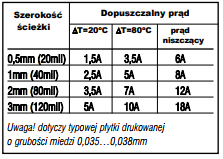
\includegraphics[width=6cm]{img/board_layouts/pcb_wire_thickness.png}
	\caption{Tabela opisująca korelację między grubością ścieżek, a maksymalnym dopuszczalnym natężęniem prądu. Źródło: \cite{pcb_wire_thickness}}
	\label{fig:image_pcb_wire_thickness}
\end{figure}
 

\begin{figure}[H]
\centering
	\subfloat[Wygląd górnej warstwy płytki]{
		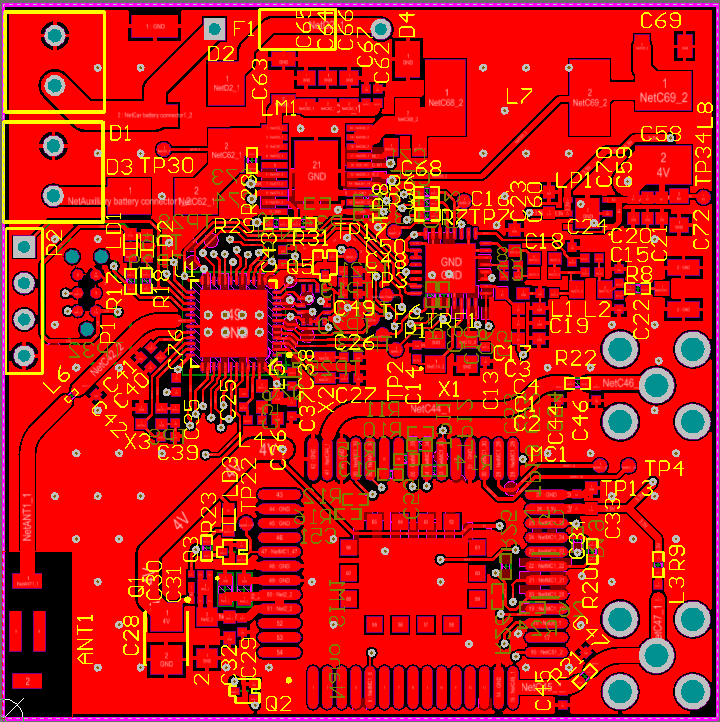
\includegraphics[width=11cm]{img/board_layouts/mainboard_top.png}
	}
	\qquad
	\subfloat[Wizualizacja górnej warstwy płytki]{
		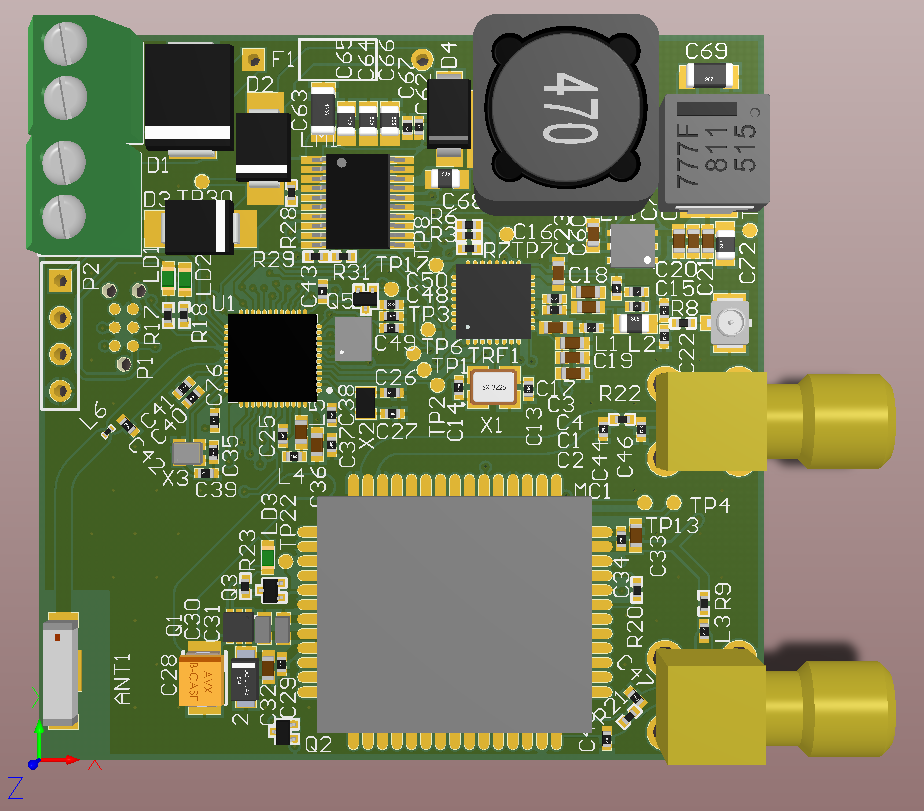
\includegraphics[width=11cm]{img/board_layouts/mainboard_visualization_top.png}
	}
	
	\caption{Wygląd górnej warstwy płytki urządzenia lokalizującego oraz jej wizualizacja. \\ Źródło: Twórczość własna}
	\label{fig:image_mainboard_top_board}
\end{figure}

\begin{figure}[H]
\centering
	\subfloat[Wygląd dolnej warstwy płytki]
	{
		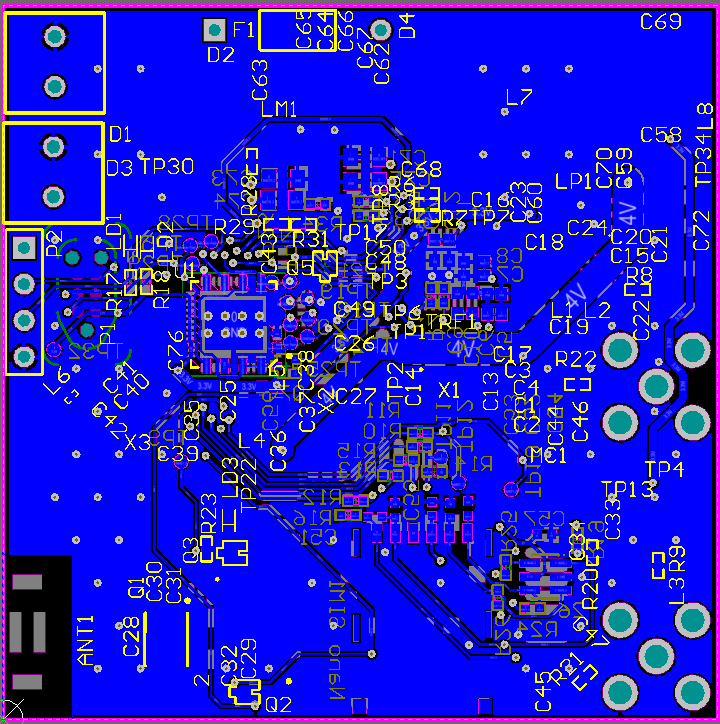
\includegraphics[width=11cm]{img/board_layouts/mainboard_bottom.png}
	}
	\qquad
	\subfloat[Wizualizacja dolnej warstwy płytki]
	{
		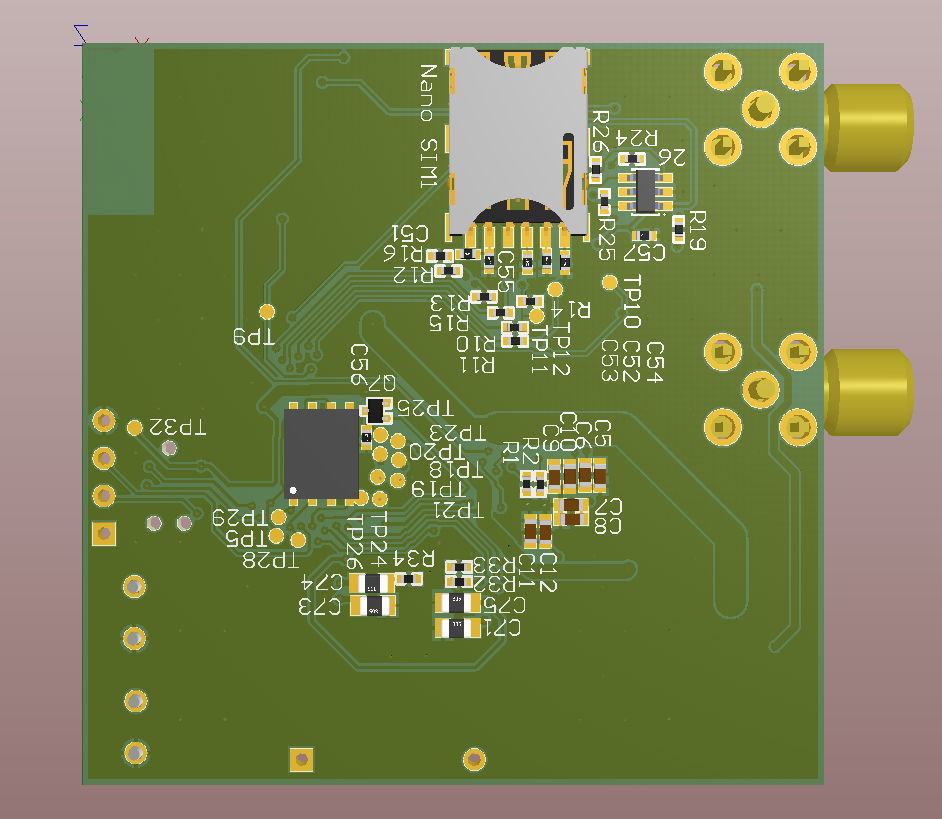
\includegraphics[width=11cm]{img/board_layouts/mainboard_visualization_bottom.png}
	}
	
	\caption{Wygląd dolnej warstwy płytki urządzenia lokalizującego oraz jej wizualizacja. \\ Źródło: Twórczość własna}
	\label{fig:image_mainboard_bottom_board}
\end{figure}
%\clearpage{\pagestyle{empty}\cleardoublepage}

\chapter{Bezpieczeństwo komunikacji}
\label{ch:communication security}

Jednym z podstawowych wymagań tej pracy jest bezpieczna wymiana komunikatów poprzez Bluetooth Low Energy. Za pomocą tego protokołu, poprzez bezprzewodowe medium, przesyłane są kluczowe dane, zwłaszcza komendy deaktywujące tryb alarmowy urządzenia. Transmisja jest zawsze realizowana rozgłoszeniowo, co powoduje, że jej podsłuchanie nie jest trudnym zadaniem. Jest to niebezpieczne z dwóch powodów. Pierwszym z nich jest fakt wysyłania wrażliwych danych, jak na przykład danych lokalizujących pojazd. Dzięki nim, potencjalny złodziej mógłby po krótkiej analizie bezproblemowo określić miejsca, w których regularnie przebywa pojazd, a następnie wybrać dla niego najbardziej korzystne i przygotować się do kradzieży. Po drugie, będąc w pobliżu pojazdu w trakcie wyłączania trybu alarmowego, byłby w stanie podsłuchać komendę deaktywującą, a następnie zapisać ją w celu późniejszego odtworzenia, co umożliwiłoby kradzież pojazdu.

Z przytoczonych powyżej powodów, komunikacja bezprzewodowa musi być szyfrowana. Jednakże operacja ta sama w sobie nie zabezpiecza komendy deaktywującej, a jedynie wrażliwe dane. Wynika to z faktu, iż w przypadku przechwycenia danych przesyłanych bezprzewodowo, dzięki szyfrowaniu są one nadal bezpieczne, ponieważ zmienny charakter. Inaczej jest w przypadku stałej komendy autoryzującej. Wynika to z faktu, że nie musi być ona tak naprawdę deszyfrowana przez potencjalnego złodzieja. Wystarczy, że jedynie ją odtworzy, nawet w formie zaszyfrowanej. Urządzenie wówczas ją zdeszyfruje i wykona deaktywację alarmu. W wyniku szyfrowania stałej komendy stałym kluczem szyfrującym, uzyskamy oczywiście również stały i powtarzalny pakiet zaszyfrowanych danych, które mogą być bezcenne w ręku potencjalnego złodzieja. W celu zabezpieczenia się przed tym, do komunikacji należy wprowadzić element zmienności w czasie.  

\section{AES}

Jako główny algorytm szyfrowania w niniejszej pracy wykorzystano algorytm AES \linebreak (\textit{ang. \textbf{A}dvanced \textbf{E}ncryption \textbf{S}tandard}) w wersji ze 128-bitowym kluczem szyfrującym.  Wyboru tego dokonano, ponieważ zastosowany w pracy mikrokontroler nRF52832 firmy Nordic Semiconductor posiada sprzetowe wsparcie szyfrowania danych wykorzystując właśnie AES128. Algorytm ten powstał w 2001 roku w Stanach Zjednoczonych w ośrodku NIST \linebreak (\textit{ang. \textbf{N}ational \textbf{I}nstitude of \textbf{S}tandards and \textbf{T}echnology}) w wyniku prac badawczych dwóch belgijskich kryptografów - Vincenta Rijmena i Joan’a Daemen, od których nazwisk powstała oryginalna nazwa algorytmu – Rijndael. Stanowi on jeden z najpopularniejszych na świecie szyfrów symetrycznych, a o jego skuteczności stanowi fakt, że w 2002r. został przyjęty jako federalny standard szyfrowania w Stanach Zjednoczonych. Pojęcie szyfr symetryczny oznacza, że do zaszyfrowania oraz zdeszyfrowania stosuje się ten sam klucz szyfrujący (w przeciwieństwie do algorytmów asymetrycznych, gdzie stosuje się dwa klucze, jeden do szyfrowania, a drugi do deszyfracji). Z tego powodu, klucz szyfrujący stanowi ekstremalnie wrażliwe dane, które pod żadnym pozorem nie powinno się przesyłać poprzez ogólno dostępne medium komunikacyjne. Wyciek klucza szyfrującego powoduje zagrożenie bezpieczeństwa komunikacji.
Proces szyfrowania składa się z kilku kroków. Pierwszym z nich jest podzielenie danych wejściowych (zwyczajowo nazywanych tekstem jawnym) na bloki o rozmiarze 128 bitów, czyli szesnastu bajtów. Każdy blok przedstawiany jest jako macierz o wymiarach 4 bajty x 4 bajty, szeregowana kolumnami. Macierze te nazywają się macierzami stanu. Następnie, na każdej z tych macierzy (bloku danych) wykonywane są kolejne operacje:

\begin{enumerate}
\item  Utworzenie podkluczy – etap ten polega na wygenerowaniu w sposób losowy klucza pierwotnego, a następnie na jego podstawie - po jednym podkluczu dla każdej z rund szyfrujących. Ich liczba jest uzależniona od rozmiaru klucza. Dla klucza 128-bitowego występuje 10 rund, dla klucza 192-bitowego – 12, a dla klucza 256-bitowego – 14 powtórzeń, wliczając klucz pierwotny.

\item Wykonanie rundy wstępnej (inicjującej). Polega na wykonaniu operacji alternatywy wyłączanej – XOR (\textit{ang. Exclusive Or}) dla każdego bajtu z bloku danych oraz odpowiadającego mu bajtu w kluczu pierwotnym.

\item Wykonanie rund szyfrujących – Etap ten jest wykonywany kilkukrotnie, w zależności od liczby cykli. Każda runda składa się z kilku kroków. 

	\begin{itemize}
	\item W pierwszym z nich, każdy bajt danych jest zastępowany innym bajtem pobranym ze zdefiniowanej tablicy (\textit{ang. lookup table}) nazywanej S-Boxe’em Rijndael’a. Operacja ta nazywa się w skrócie SB (\textit{ang. \textbf{S}ubstitude \textbf{B}ytes}) i przedstawiono ją na rysunku \ref{fig:image_substitute_bytes}. Zgodnie z zamysłem twórców, tablica ta gwarantuje nieliniowość przekształcenia, a w efekcie i całego szyfrowania.
	
	\begin{figure}[h]
		\centering
		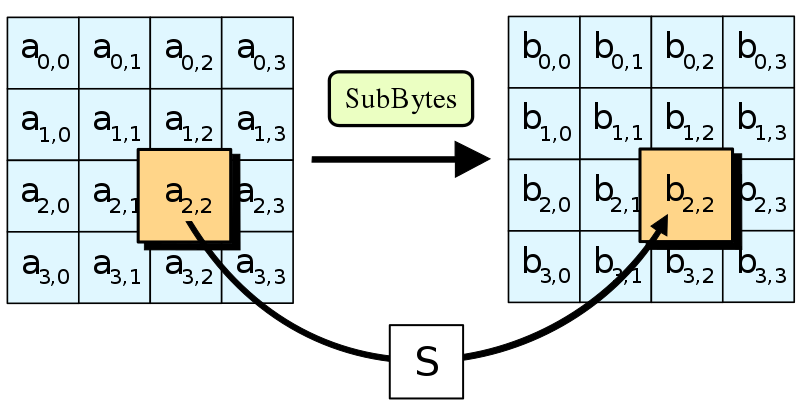
\includegraphics[width=10cm]{img/com_security/800px-AES-SubBytes.png}
		\caption{Wykonanie operacji Substitute Bytes. Źródło: \cite{aes_wiki}.}
		\label{fig:image_substitute_bytes}
	\end{figure}

	\item  Kolejny krok to zamiana wierszy. Polega na przesunięciu bajtów w trzech ostatnich wierszach bloku. Pierwszy wiersz pozostaje bez zmian, w drugim wierszu bajty są przesuwane o jeden w lewo, w trzecim o dwie pozycje w lewo, a w ostatnim o 3 miejsca w tym samym kierunku. Każdy bajt, który w wyniku przesunięcia znajdzie się poza wierszem, zostaje umieszczony na jego ostatniej pozycji (wiersze w wyniku rotacji się zawijają). Operacja ta nosi miano SR (\textit{ang. \textbf{S}hift \textbf{R}ows}). Przedstawiono ją na rysunku \ref{fig:image_shift_rows}.
	
	\begin{figure}[h]
		\centering
		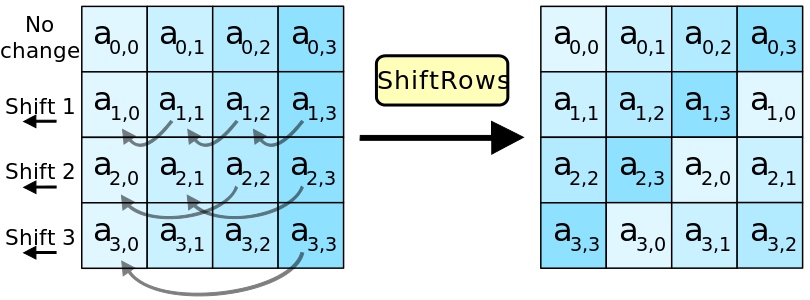
\includegraphics[width=10cm]{img/com_security/810px-AES-ShiftRows.png}
		\caption{Wykonanie operacji Shift Rows. Źródło: \cite{aes_wiki}.}
		\label{fig:image_shift_rows}
	\end{figure}
	
	\item Trzecim z kolei krokiem jest operacja mieszania kolumn – MC (\textit{ang. \textbf{M}ix \textbf{C}olumns}). W tym etapie, każda z kolumn jest przemnażana lewostronnie przez stałą macierz o wymiarach 4 x 4, w wyniku czego powstaje kolumna z nowymi wartościami. Operacja ta przedstawiona jest na rysunku \ref{fig:image_mix_columns}.
	
	\begin{figure}[H]
		\centering
		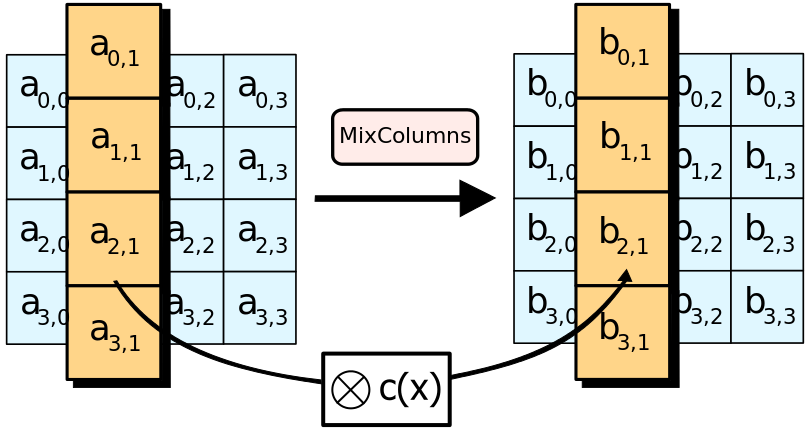
\includegraphics[width=10cm]{img/com_security/810px-AES-MixColumns.png}
		\caption{Wykonanie operacji Mix Columns. Źródło: \cite{aes_wiki}.}
		\label{fig:image_mix_columns}
	\end{figure}
	
	\item Ostatni krok nazywany jest AR (\textit{ang. \textbf{A}dd \textbf{R}ound Key}) i polega na wykonaniu operacji XOR na każdym bajcie bloku danych i odpowiadającym mu bajcie w kluczu przypisanym do danej rundy. Wizualizację kroku przedstawiono na rysunku \ref{fig:image_round_keys}.
	
	\begin{figure}[h]
		\centering
		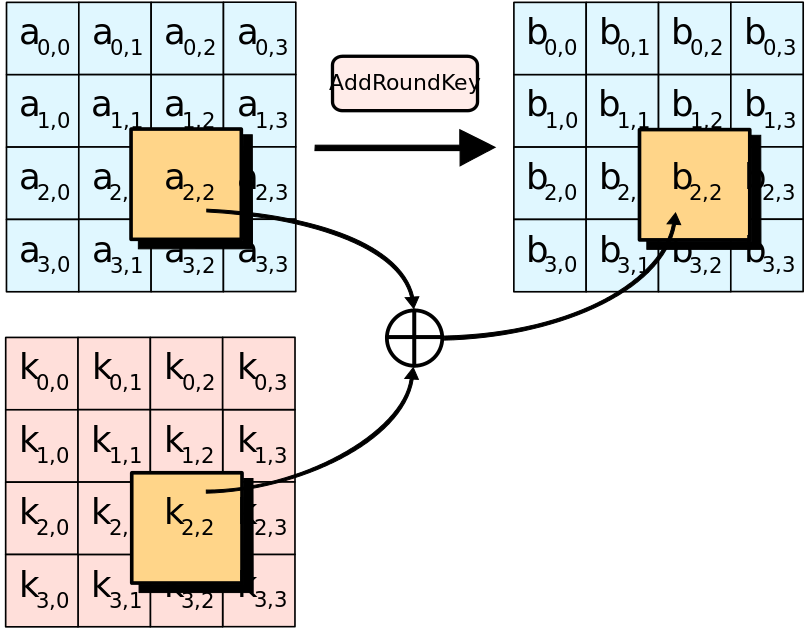
\includegraphics[width=10cm]{img/com_security/810px-AES-AddRoundKey.png}
		\caption{Wykonanie operacji Add Round Key. Źródło: \cite{aes_wiki}.}
		\label{fig:image_round_keys}
	\end{figure}
	\end{itemize}
	
\item Ostatni etap to runda kończąca – W jej trakcie wykonywane są operacje identyczne jak w rundach szyfrujących, za wyłączeniem mnożenia kolumn, które nie występuje.

\end{enumerate}

Deszyfrowanie jest operacją odwrotną do szyfrowania i polega na przekształceniu danych zaszyfrowanych na tekst jawny. Tak samo jak w przypadku szyfrowania, tekst dzieli się na 16-bajtowe bloki. W jego trakcie wykonuje się analogiczne operacje co w przypadku szyfrowania.

\begin{enumerate}
\item Odwrotne podstawianie bajtów – polega na ponownym zastosowaniu tablicy S-Box w celu podmiany bajtów.

\item Przesuwanie bajtów w wierszach w prawo. Zasada jest taka sama jak w operacji SR, zmienia się jedynie kierunek.

\item Wykonanie operacji XOR dla każdego bajtu bloku danych z odpowiadającym mu bajtem w podkluczu przypisanym do danej rundy deszyfrującej. Podklucze są takie same jak w trakcie szyfrowania, lecz powinny być brane w kolejności odwrotnej (zaczynając od ostatniego, a kończąc na kluczu pierwotnym).

\item Ostatnia operacja to odwrócone mnożenie kolumn.

\end{enumerate}

W efekcie uzyskujemy blok danych zdeszyfrowanych.
Przedstawiony tutaj wariant algorytmu szyfrowania nosi miano ECB (\textit{ang. \textbf{E}lectronic \textbf{C}ode\textbf{b}ook}) i stanowi najprostszą metodę szyfrowania. Można go przedstawić na rysunkach \ref{fig:image_ecb_encrypt} oraz \ref{fig:image_ecb_decrypt}.

	\begin{figure}[h]
		\centering
		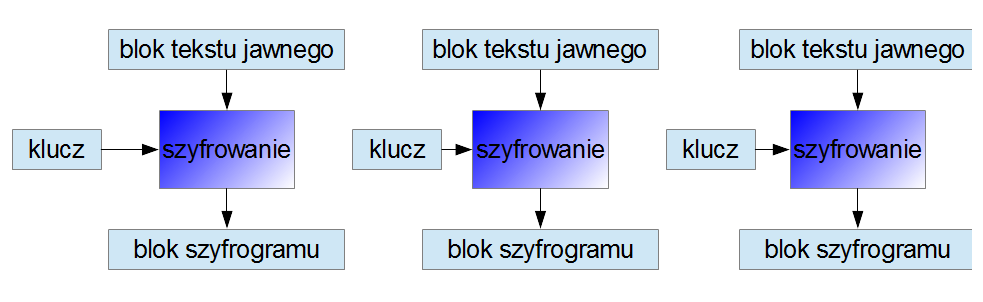
\includegraphics[width=15cm]{img/com_security/ECB_szyfrowanie.png}
		\caption{Operacja szyfrowania metodą ECB. Źródło: \cite{aes_cryptoit}.}
		\label{fig:image_ecb_encrypt}
	\end{figure}
	
	\begin{figure}[h]
		\centering
		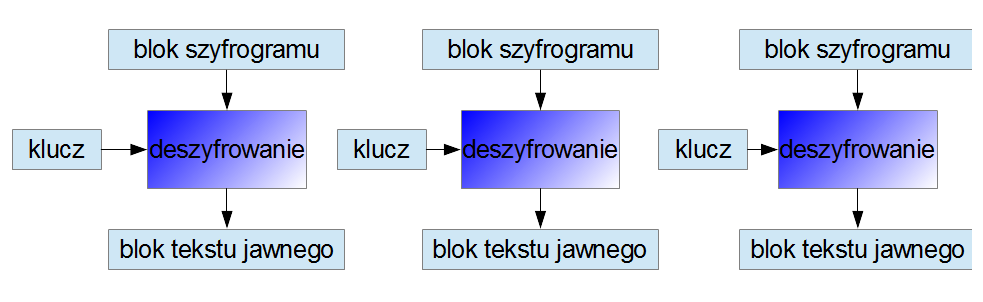
\includegraphics[width=15cm]{img/com_security/ECB_deszyfrowanie.png}
		\caption{Operacja deszyfrowania metodą ECB. Źródło: \cite{aes_cryptoit}.}
		\label{fig:image_ecb_decrypt}
	\end{figure}
	
Czas trwania szyfrowania pojedynczego bloku danych o długości szesnastu bajtów na mikrokontrolerze nRF52832 wynosi w przybliżeniu 30 $\mu s$. Deszyfrowanie trwa zaś około 60 $\mu s$.


\section{Dodatkowe warianty szyfrowania AES}

Jak zostało przedstawione wcześniej, mechanizmy szyfrowania doskonale działają w przypadku wrażliwych danych. Nie sprawdzają się natomiast w przypadku przesyłania komend, ze względu na brak zmienności pakietów w czasie i możliwości odtworzenia zaszyfrowanego pakietu przez niepowołane osoby. Z tego powodu, do komunikacji należy wprowadzić element zmienności.
Jednym z wariantów algorytmu AES jest tzw. CFB (\textit{ang. \textbf{C}ipher \textbf{F}eed\textbf{b}ack}), przedstawiony na rysunkach \ref{fig:image_cfb_encrypt} oraz \ref{fig:image_cfb_decrypt}. Stanowi on wysokopoziomowy algorytm, który bazuje na wariancie ECB, zmieniając jedynie logiczną strukturę informacji niezbędnych do szyfrowania. Przede wszystkim, wprowadza pojęcie wektora inicjującego (\textit{ang. initializing vector}), który stanowi niezbędny dodatkowy element zmienności. Klucz główny jest zazwyczaj niezmienny dla pary komunikujących się ze sobą urządzeń, co w rezultacie wprowadza konieczność nieupubliczniania go. Wektor inicjujący jest natomiast generowany przy każdej nowej komunikacji. 

	\begin{figure}[h]
		\centering
		\includegraphics[width=15cm]{img/com_security/CFB_szyfrowanie.png}
		\caption{Operacja szyfrowania metodą CFB. Źródło: \cite{aes_cryptoit}.}
		\label{fig:image_cfb_encrypt}
	\end{figure}
	
	\begin{figure}[h]
		\centering
		\includegraphics[width=15cm]{img/com_security/CFB_deszyfrowanie.png}
		\caption{Operacja deszyfrowania metodą CFB. Źródło: \cite{aes_cryptoit}.}
		\label{fig:image_cfb_decrypt}
	\end{figure}
	

W odróżnieniu od wariantu ECB, zamiast tekstu jawnego szyfrowaniu ulega wektor inicjujący. Jego postać zaszyfrowana jest następnie poddawana operacji XOR z blokiem danych tekstu jawnego, a powstały w ten sposób szyfrogram stanowi nowy wektor inicjujący dla następnego bloku danych.
W przypadku deszyfrowania korzysta się oczywiście z tego samego wektora inicjującego oraz klucza szyfrującego. Co ciekawe, w odróżnieniu od wariantu ECB, w metodzie CFB deszyfrowanie jest to tak naprawdę szyfrowanie. Oznacza to, że wystarczy zaimplementować jedynie mechanizm szyfrowania w algorytmie AES, aby móc zarówno szyfrować jak i deszyfrować wiadomości. Zaszyfrowany wektor inicjujący jest poddawany operacji XOR z blokiem tekstu zaszyfrowanego w efekcie czego uzyskujemy blok tekstu jawnego. Natomiast blok tekstu zaszyfrowanego stanowi wektor inicjujący dla następnych bloków szyfru.


\section{Realizacja szyfrowania komunikacji w projekcie}
W pracy zdecydowano się na wykorzystanie zarówno metod ECB oraz CFB. Pierwszym, a zarazem najbardziej podstawowym etapem jest generowanie klucza szyfrującego. Operacja ta jest realizowana przez płytę główną systemu lokalizującego. Następnie, klucz jest przekazywany w trakcie inicjalizacji porzez interfejs NFC (\textit{ang. \textbf{N}ear \textbf{F}ield \textbf{C}ommunication}) do urządzenia deaktywującego, pełniącego rolę beacona (urządzenia rozgłaszającego). Zastosowanie NFC jest powszechnie uważane za bezpieczną metodę komunikacji, ze względu na jej bardzo niską moc transmisji, a tym samym bardzo niewielki zasięg (do 10 cm). Ogranicza to zatem możliwość podsłuchania klucza szyfrującego do zera. Przy pomocy tego klucza, za każdym razem gdy płyta główna systemu połączy się z urządzeniem deaktywującym w celu uzyskania od niego komendy deaktywującej, wpierw wysłany zostanie zaszyfrowany, nowo wygenerowany na potrzeby danego połączenia wektor inicjalizacyjny. Umożliwi to dalszą komunikację wykorzystując wariant CFB oraz niezbędną zmienność zaszyfrowanych pakietów, praktycznie niwelującą skuteczność podsłuchiwania transmisji. 
%\clearpage{\pagestyle{empty}\cleardoublepage}

\chapter{Oprogramowanie}
\label{software}

\section{Urządzenie dezaktywujące}



\clearpage

\section{Urządzenie lokalizujące}
\lstset{language=C}

Urządzenie lokalizujące realizuje następujące funkcje: 

\begin{itemize}
\item wygenerowanie głównego klucza szyfrującego i sparowanie z urządzeniem deaktywującym,
\item zapewnienie bezpiecznego kanału komunikacji w trakcie połączenia z \textit{Key Tag'iem},
\item wykrywanie ruchu pojazdu,
\item komunikacja z urządzeniem deaktywującym, w celu podjęcia próby deaktywacji alarmu,
\item alarmowe powiadamianie właściciela w przypadku nieautoryzowanego przemieszczenia pojazdu,
\item pobieranie próbek lokalizacji, prędkości, przyspieszenia, a  także aktualnego kursu (azymutu) i innych parametrów po wykryciu ruchu oraz ich cykliczne wysyłanie na zdalny serwer danych,
\item analiza stylu jazdy kierowcy,
\item wysyłanie poprzez SMS lokalizacji pojazdu na żądanie użytkownika.
\end{itemize}

\clearpage
Duża liczba zadań realizowanych przez mikrokontroler sterujący oraz konieczność wywoływania ich po ściśle określonej sekwencji czasowej spowodowała, że niezbędnym stało się wprowadzenie modułu planisty. Stanowi on bardzo prostą funkcjonalność, bez możliwości wywłaszczania zadań i zmiany kontekstu, więc nie wprowadza wielowątkowości znanej z pełnoprawnych systemów operacyjnych. Jego celem jest zakolejkowanie zadań, oznaczenie ich jako gotowych do wykonania po upływie wymaganego czasu, a następnie wykonaniu ich przy pierwszej sposobności po wyjściu programu z przerwania. Kod służący do  kolejkowania zadań przedstawiono na listingu \ref{listing_scheduler_add}. Na listingu \ref{listing_scheduler_check} umieszczono funkcję, która jest cyklicznie wywyływana (co 10 ms) w przerwaniu generowanym przez energooszczędny timer. Jej zadaniem jest oznaczenie zadań, które można już wykonać. Na ostatnim listingu, oznaczonym numerem  \ref{listing_scheduler_exec}, przedstawiono procedurę wykonującą oczekujące zadania. Ograniczeniem funkcjonalnym jest tutaj fakt, iż żadne z zadań nie może przyjmować argumentów, ani zwracać wartości. 
\clearpage

\begin{lstlisting}[label=listing_scheduler_add, caption=Funkcja do kolejkowania zadań]

scheduler_error_code_e SchedulerAddOperation(void (*callback)(void),
	 										volatile	uint32_t timeMsFromNow,
	 										volatile uint8_t* taskIndex,
	 										bool isCyclic){
    scheduler_entry_t entry;

    // Just safe guard not to miss the time
    if (timeMsFromNow < 2)
    {
        timeMsFromNow = 2;
    }

    for (uint8_t i=0; i< SCHEDULER_BUFFER_SIZE; ++i)
    {
        if (_scheduleBuffer[i].isInProgress == false)
        {
            entry.isInProgress = true;
            entry.isTimedOut = false;
            entry.callback = callback;
            entry.timePeriodMs = timeMsFromNow;
            entry.triggerTime = scheduler_current_time_ms + timeMsFromNow;
            entry.isCyclic = isCyclic;
            memcpy(&_scheduleBuffer[i], &entry, sizeof(scheduler_entry_t));
            if (taskIndex != NULL)
                *taskIndex = i;
            return E_SCHEDULER_OK;
        }
    }

    return E_SCHEDULER_NO_RESOURCES;
}
\end{lstlisting}

\clearpage
\begin{lstlisting}[label=listing_scheduler_check, caption=Funkcja do sprawdzania czy nie należy wykonań zadania]

scheduler_error_code_e SchedulerCheckOperations(){
    scheduler_current_time_ms += 10;
    for (uint8_t i=0; i< SCHEDULER_BUFFER_SIZE; ++i)
    {
        if (_scheduleBuffer[i].isInProgress == true &&
            _scheduleBuffer[i].triggerTime <= scheduler_current_time_ms)
        {
            // If it is cyclic task - reschedule the next cycle
            if (_scheduleBuffer[i].isCyclic)
            {
                _scheduleBuffer[i].triggerTime = scheduler_current_time_ms 
                +_scheduleBuffer[i].timePeriodMs;
            }

            _scheduleBuffer[i].isTimedOut = true;
        }
    }

    return E_SCHEDULER_OK;
}
\end{lstlisting}


\begin{lstlisting}[label=listing_scheduler_exec, caption=Funkcja do wykonywania zadań]

scheduler_error_code_e ScheduleExecutePendingOperations(){
    for (uint8_t i=0; i< SCHEDULER_BUFFER_SIZE; ++i)
    {
        if (_scheduleBuffer[i].isInProgress == true && 
        		_scheduleBuffer[i].isTimedOut == true)
        {
            if (_scheduleBuffer[i].isCyclic == false)
            {
                _scheduleBuffer[i].isInProgress = false;
            }
            _scheduleBuffer[i].callback();
            _scheduleBuffer[i].isTimedOut = false;
        }
    }

    return E_SCHEDULER_OK;
}

\end{lstlisting}

Główny cykl działania urządzenia został przedstawiony na rysunku \ref{fig:image_soft_mainboard_main_alghoritm}.

\begin{figure}[H]
	\centering
	\includegraphics[width=16cm]{img/software/mainboard/Tracking_alghoritm.jpg}
	\caption{Główny algorytm działania urządzenia. 
	\\Źródło: Opracowanie własne.}
	\label{fig:image_soft_mainboard_main_alghoritm}
\end{figure}

Jak widać na rysunku \ref{fig:image_soft_mainboard_main_alghoritm}, po uruchomieniu i zainicjalizowaniu peryferiów i modułów na płytce, mikrokontroler dokonuje sprawdzenia czy wygenerowany został klucz szyfrujący, służący do zabezpieczenia komunikacji z dedykowanym urządzeniem deaktywującym. Jeśli klucza nie ma, to oznacza że urządzenie nie zostało jeszcze sparowane. Wówczas, włączony zostaje układ NFC, procesor wchodzi w tryb oszczędzania energii w trakcie oczekiwania na parowanie, a całe urządzenie przechodzi w stan nieoperacyjny, dopóki nie zostanie powiązane z modułem deaktywującym. Algorytm komunikacji został przedstawiony w podrozdziale \ref{key_tag} na rysunku \ref{fig:image_soft_keytag_key exchange}. Po deaktywacji, moduł NFC zostaje wyłączony i nie jest używany aż do momentu powrotu do ustawień fabrycznych, a mikrokontroler wchodzi w tryb oszczędzania energii w oczekiwaniu na nadchodzące zadania.

Pierwszym z nich jest wykrywanie ruchu pojazdu. Zostało to zrealizowane poprzez wykorzystanie funkcji akcelerometru - wybudzenia w razie wykrycia przyspieszenia powyżej programowalnego progu, które utrzymywałoby się przez pewien konfigurowalny czas. W wyniku badań eksperymentalnych, został on ustalony na wartość 0,9 $\frac{m}{s^2}$, trwającą przez więcej niż 1 sekundę, co pozwala na wykrycie drgań spowodowanych zamknięciem drzwi pojazdu. Akcelerometr jest cykliczne (co 5 sekund) odpytywany przez mikrokontroler, w celu sprawdzenia czy nie nastąpił ruch pojazdu. Jeśli nie zostało to wykryte, to mikrokontroler przechodzi do trybu oszczędzania energii i cały cykl się powtarza. Jeśli wykryto ruch, zadanie okresowego sprawdzania przemieszczenia jest wyłączane, natomiast do kolejki zadań ładowane są 3 najważniejsze z punktu widzenia całego systemu procedury - zadanie alarmu, skanowania w poszukiwaniu \textit{Key Tag'a} oraz cyklicznego pobierania próbek lokalizacji. Pierwsze z nich stanowi zegar, który odlicza 30 sekund. Jeśli w tym czasie, alarm zostanie deaktywowany poprzez nawiązanie połączenia z urządzeniem dezaktywującym i nadanie odpowiedniego komunikatu, wówczas zadanie zostaje anulowane i jedynym cyklicznym zadaniem jest próbkowanie lokalizacji. W przeciwnym razie, uruchamiane jest zadanie cyklicznego, co 10 minutowego powiadamiania właściciela o lokalizacji pojazdu poprzez wiadomości SMS. Okres ten został dobrany w ten sposób, aby nie wyczerpać za szybko śródków na koncie karty SIM, użytej w module, a przy tym uzyskać rozsądną częstotliwość wysyłania SMS'ów. Zadanie to można anulować, w przypadku fałszywego alarmu, wysyłając odpowiednią komendę poprzez SMS z numeru właściciela. 

Kolejne zadanie to alarm w Pierwszy krok w procesie deaktywacji alarmu jest wykonywany przez płytkę główną. Ze względu na fakt, iż urządzenie powinno być ukryte, nie powinno ono rozgłaszać żadnych pakietów w sposób ciągły, co zminimalizuje jego wykrywalność w aplikacjach skanujących poprzez Bluetooth Low Energy. Z tego powodu, w momencie wykrycia ruchu pojazdu, to ono nawiązuje połączenie z \textit{Key Tag'iem}. W tym celu dokonuje skanowania urządzeń posiadających odpowiedni zestaw serwisów i charakterystyk. Dla każdego z nich, sprawdza jego nazwę. Jeśli urządzenie ma odpowiednią nazwę, dopiero wówczas nawiązywane jest z nim połączenie. W trakcie połączenia, urządzenie peryferyjne musi przesłać kod deaktywujący (wygenerowany w trakcie parowania), zaszyfrowany kluczem szyfrowania wygenerowanym na potrzeby danego połączenia. Jeśli zostanie on poprawnie odszyfrowany, alarm jest deaktywowany. W przeciwnym razie - połączenie zostaje zerwane. Algorytm deaktywowania alarmu przedstawiono w rozdziale \ref{key_tag} na rysunku \ref{fig:image_soft_keytag_alarm_deactivation}.

Ponadto, niezależnie od tego czy alarm został deaktywowany czy nie, uruchamiane jest zadanie cyklicznego pobierania próbek lokalizacji. Okres próbkowania wynosi 10 sekund i w momencie pobierania informacji gromadzone są dane takie jak:

\begin{itemize}
\item status lokalizacji,
\item lokalizacja pojazdu,
\item prędkość pojazdu,
\item średnie przyspieszenie pojazdu z okresu pomiędzy próbkami,
\item azymut ruchu,
\item ocena jazdy z okresu pomiędzy próbkami,
\item parametr HDOP informujący o jakości sygnału GPS,
\item liczba satelitów z których odebrano sygnał,
\item czas pobrania próbki.
\end{itemize}

Na rysunku \ref{fig:image_soft_mainboard_control_flow} przedstawiono diagram interakcji, który pokazuje przepływ sterowania pomiędzy zadaniami. 


\begin{figure}[H]
	\centering
	\includegraphics[width=17cm]{img/software/mainboard/MainBoardStartTracking.jpg}
	\caption{Przepływ sterowania w przypadku wykrycia ruchu pojazdu. 
	\\Źródło: Opracowanie własne.}
	\label{fig:image_soft_mainboard_control_flow}
\end{figure}
\clearpage

\section{Aplikacja mobilna}

\clearpage

\section{Aplikacja serwerowa}

Kolejnym etapem pracy było projekt aplikacji serwerowej, która obsługiwałaby zapytania HTTP (\textit{ang. \textbf{H}yper\textbf{t}ext \textbf{T}ransfer \textbf{P}rotocol}) użytkownika oraz zapytania kierowane do bazy danych. Aplikacja została napisana w środowisku Qt. Wybór środowiska nastąpił z kilku powodów. Pierwszym i jednocześnie najważniejszym z nich jest wbudowany moduł obsługi relacyjnych baz danych. Dzięki temu, wykorzystując kilka wysokopoziomowych funkcji można szybko operować na zgromadzonych danych. Ponadto, aplikacja napisana w C++ statystycznie zapewnia większą wydajność niż podobna napisana w języku Java. Ostatnim z powodów jest znajomość tej biblioteki oraz jej metodologii komunikacji wewnętrznej przez autora pracy.

Aplikacja składa się z dwóch głównych modułów: manager'a bazy danych oraz serwera HTTP.

Baza danych składa się z 4 tabel. Są to :

\begin{itemize}
\item tabela użytkowników,
\item tabela urządzeń,
\item tabela tras,
\item tabela próbek.
\end{itemize}

Jako silnik bazodanowy zdecydowano się wykorzystać system SQLite. Stanowi on uproszczony, lecz bardzo wydajny sterownik opierający się na zapytaniach SQL, służący do obsługi relacyjnych baz danych. Kolejną zaletą jest fakt, iż jest on obsługiwany wewnętrznie przez bibliotekę Qt.
Relacje pomiędzy poszczególnymi tabelami bazy danych zostały przedstawione na rysunku \ref{fig:image_soft_db_relations}.

Założenia struktury bazy danych są następujące.

\begin{itemize}
\item Każdy zarejestrowany użytkownik może posiadać więcej niż jedno urządzenie.
\item Każde urządzenie może otrzymać opisującą je krótką nazwę.
\item Do każdego z urządzeń może być przypisana więcej niż jedna trasa.
\item Wpis trasy posiada wpisy o miejscach i czasach ich rozpoczęcia i zakończenia, oraz zbiór przypisanych do niej próbek lokalizacji zbieranych cyklicznie w czasie jej trwania.
\end{itemize}

\begin{figure}[H]
	\centering
	\includegraphics[width=17cm]{img/software/database/Database_relations.jpg}
	\caption{Schemat relacji między tabelami w bazie danych. 
	\\Źródło: Opracowanie własne.}
	\label{fig:image_soft_db_relations}
\end{figure}

Jako serwer HTTP zastosowano bibliotekę QttpServer autorstwa użytkownika supamii \cite{qttpserver}. Została ona napisana pod licencją MIT, co zapewnia swobodę użytkowania i modyfikacji kodu źródłowego, a nawet komercyjne zastosowanie pod warunkiem umieszczenia oryginalnych warunków licencyjnych i informacji o autorze. Biblioteka umożliwia komunikację zarówno poprzez zapytania HTTP typu GET jak i POST. Zapytania te różnią się pomiędzy sobą tym, że w zapytaniu typu GET zmienne przekazywane są jawnie wewnątrz adresu URL, natomiast w zapytaniu typu POST są one ukryte.

Przy pomocy aplikacji, można wykonać następujące operacje:

\begin{itemize}
\item logowanie użytkownika,
\item wylogowanie użytkownika,
\item rejestracja nowego użytkownika,
\item pobieranie danych o użytkowniku z bazy danych,
\item zmianę danych użytkownika,
\item zmianę hasła użytkownika,
\item kasowanie konta użytkownika,
\item dodawanie urządzenia do konta użytkownika,
\item pobieranie listy urządzeń przypisanych do użytkownika,
\item pobieranie informacji o urządzeniu,
\item usuwanie urządzenia z bazy danych,
\item dodawanie nowej trasy do urządzenia,
\item pobieranie listy tras przypisaych do urządzenia,
\item pobieranie informacji o trasie,
\item dodawanie próbek do trasy,
\item zakończanie trasy,
\item usuwanie trasy.
\end{itemize}
\clearpage

\section{Strona internetowa}
\lstset{language=HTML, inputencoding=utf8, breaklines=true}

Ostatnim elementem systemu opisywanego w tej pracy jest strona interetowa. Dzięki niej, możliwy staje się zdalny i czytelny podgląd danych, które napływają praktycznie w czasie rzeczywistym. Z tego względu stanowi ona równie istotną część pracy co pozostałe. Dzięki wykorzystaniu strony internetowej, możliwe staje się stworzenie konta użytkownika, przypisanie do niego urządzeń, a następnie podgląd tras - zarówno aktualnie przebywanej jak i historycznych wraz z ich parametrami, zapisanymi na serwerze.

Szkielet strony internetowej został zaprojektowany w języku HTML (\textit{ang. \textbf{H}yper\textbf{t}ext \textbf{M}arkup \textbf{L}anguage}), natomiast jej część funkcjonalna przy użyciu języka \textit{JavaScript}. Jest to język skryptowy, wykorzystywany głównie w przeglądarkach i charakteryzuje się tym, że jest jednowątkowy.

Dzięki wykorzystaniu JavaScript, możliwe staje się dodanie wielu funkcjonalności do struktury strony internetowej, które stanowią jej połączenie ze światem zewnętrznym, oraz umożliwiają wykorzystanie wielu efektownych rozwiązań wizualnych, jak na przykład animowane przewijanie strony, wyskakujące okienka czy interaktywne wykresy.

W niniejszej pracy, dzięki wykorzystaniu JavaScript możliwe stało się połączenie strony internetowej z bazą danych w celu użycia wymienionych w poprzednim podrozdziale funkcji.  

Na rysunkach \ref{fig:image_soft_website_login}, \ref{fig:image_soft_website_register_user}, \ref{fig:image_soft_website_main_page} oraz \ref{fig:image_soft_website_track_map} przedstawiono podstawowe ekrany: logowania, rejestracji użytkownika, ekran główny oraz ekran trasy.

\begin{figure}[H]
	\centering
	\includegraphics[width=8cm]{img/software/website/login_window.png}
	\caption{Strona logowania. Źródło: Twórczość własna}
	\label{fig:image_soft_website_login}
\end{figure}

\begin{figure}[H]
	\centering
	\includegraphics[width=17cm]{img/software/website/register_user.png}
	\caption{Ekran rejestracji użytkownia. Źródło: Twórczość własna}
	\label{fig:image_soft_website_register_user}
\end{figure}

\begin{figure}[H]
	\centering
	\includegraphics[width=18cm]{img/software/website/main_screen.png}
	\caption{Strona główna. Źródło: Twórczość własna}
	\label{fig:image_soft_website_main_page}
\end{figure}

\begin{figure}[H]
	\centering
	\includegraphics[width=18cm]{img/software/website/main_screen.png}
	\caption{Okno trasy. Źródło: Twórczość własna}
	\label{fig:image_soft_website_track_map}
\end{figure}

Ekran trasy przedstawia poszczególne próbki lokalizacji, należące do trasy, na mapie od firmy Google. W tym celu, niezbędne staje się wykorzystanie API producenta dla modułu Google Maps. Pozwala ono na wyświetlenie mapy, przybliżanie i oddalanie, odnalezienie lokalizacji, naniesienie znaczników (w tym autorskich - zdefiniowanych w formacie grafiki wektorowej - \textit{.svg}). Ponadto, dzięki zastosowaniu modułu \textit{Info Bubble}, możliwe staje się wyświetlenie na mapie interaktywnego okienka informacyjnego, powiązanego z konkretnym znacznikiem geolokalizacyjnym.

Aby wykorzystać API Google Maps, należy zarejestrować aplikację na stronie \url{https://developers.google.com/maps/documentation/javascript/get-api-key}. Po rejestracji, do projektu przypisany zostanie klucz, który należy zawrzeć wewnątrz zapytania HTTP wykonywanego przy ładowaniu strony, umożliwiającego ściągnięcie z internetu plików źródłowych zawierających kod obsługujący mapy. Przedstawiono to na listingu \ref{listing_google_map_api}.

\begin{lstlisting}[label=listing_google_map_api, caption=Fragment kodu pozwalający na użycie API Google Maps]
<script async defer src="https://maps.googleapis.com/maps/api/js?key=TWOJ_KLUCZ_API&callback=initMap" type="text/javascript"></script>
\end{lstlisting}

Na listingach \ref{listing_http_api_post} oraz \ref{listing_http_api_get} przedstawiono fragmenty kodu, które umożliwiają wysłanie zapytań HTTP typu POST oraz GET. Stanowią one podstawową formę komunikacji między stroną internetową, a serwerem bazodanowym.

\begin{lstlisting}[label=listing_http_api_post, caption=Fragment kodu pozwalający na użycie zapytań HTTP typu POST]
function http_post(_url, _arguments, _successCallback)
{
  var _args = JSON.stringify(_arguments);
  // Send the data using post
  $.ajax({
    url: _url,
    type: "POST",
    dataType: "json", // expected format for response
    contentType: "application/json", // send as JSON
    data: _args ,

    complete: function() {
      //called when complete
    },
    success: function(msg) {
      _successCallback(msg);
    },
    error: errorCallback,
    });
}
\end{lstlisting}

\clearpage

\begin{lstlisting}[label=listing_http_api_get, caption=Fragment kodu pozwalający na użycie zapytań HTTP typu GET]
function http_get(_url, _arguments, _successCallback)
{
  //var _args = JSON.stringify(_arguments);
  var _args = _arguments;
  // Send the data using post
  $.ajax({
    url: _url,
    type: "GET",
    dataType: "json", // expected format for response
    contentType: "application/json", // send as JSON
    data: _args ,

    complete: function() {
      //called when complete
    },
    success: function(msg) {
      _successCallback(msg);
    },
    error: errorCallback,
    });
}
\end{lstlisting}




%\clearpage{\pagestyle{empty}\cleardoublepage}

\chapter{Analiza stylu jazdy}

\section{Wstęp}

Niniejszy rozdział stanowi opis dodatkowej funkcjonalności oferowanej w zaprojektowanym w pracy urządzeniu. Zawarte są w nim autorskie badania, krótki opis istniejących rozwiązań oraz propozycja własnego algorytmu wraz z jego rezultatami. 

Funkcjonalność opisująca styl jazdy kierowcy pojazdu jest niezwykle istotna z punktu widzenia jednej z grup docelowych, do których kierowane jest urządzenie - firm posiadających flotę pojazdów. Dzieje się tak, ze względu na rosnące koszty prowadzenia działalności oraz użytkowania pojazdów (wzrost cen paliwa, części zamiennych i usług, a także niezbędnych ubezpieczeń OC) co wprowadza konieczność ograniczenia zbędnych wydatków. Można do nich zaliczyć nadmiernie szybkie zużycie części eksploatacyjnych jak na przykład klocki hamulcowe czy opony, a także koszty związane z wypadkami losowymi takimi jak stłuczki. W przypadku firm, są one często generowane przez nieodpowiedzialnych pracowników, którzy nie szanują własności pracodawcy i prowadzą w sposób lekkmyślny, agresywny. Ograniczenie tego procederu jest o tyle problematyczne, iż trudno o jednoznaczne dowody winy pracownika - kierowcy. Odpowiadając na tę potrzebę rynkową, opisywane w tej pracy system umożliwia nie tylko ocenę stylu jazdy na bieżąco i jej zdalny podgląd, lecz także zapisywanie historii ocen, przypisanych do punktów trasy przebytej przez pracownika wraz z dodatkowymi parametrami, opisywanymi we wcześniejszych rozdziałach. Pozwala to nie tylko na wskazanie, iż pracownik jechał nadto agresywnie, lecz także informację kiedy i gdzie to nastąpiło.

\section{Istniejące metody}

W ramach przygotowania do implementacji algorytmu analizy stylu jazdy, dokonano przeglądu artykułów opisujących różne metody. Najciekawszy z nich (\cite{driving_analysis_article}), opisuje wykorzystanie telefonu typu smartphone jako platformy czujników pomiarowych. Metoda opisana w artykule jest bardzo podobna do sposobu wykrywania gestów w kontrolerach ruchu.  Wykorzystywane są w tym celu dane z akcelerometru oraz żyroskopu oraz system GPS. Pierwsze dwa z nich umożliwiają wykrycie łagodnych i ostrych skrętów, manewru zawracania, przyspieszania i hamowania. Moduł GPS służy do wykrycia prędkości pojazdu. Głównym algorytmem wykrywania jest DTW (\textit{ang. \textbf{D}ynamic \textbf{T}ime \textbf{W}arping}), który służy do wyznaczenia miary podobieństwa między dwoma sygnałami. 
Autorzy umieszczają telefon na desce rozdzielczej i odpowiednio go orientują względem pojazdu. Działający na nim program dokonuje filtracji danych filtrem dolnoprzepustowym o częstotliwości 25 Hz ze względu na drgania pojazdu pochodzące od pracującego silnika. Dane zbierane są w postaci zbioru kilku tysięcy próbek. 
Pierwszym etapem jest rozpoczęcie wykrycia manewru. W tym celu zastosowano średnią kroczącą:

\begin{equation}
	SMA = \frac{g(i)^2 + g(i-1)^2 + ... + g(i-k-1)^2}{k}
\end{equation}

gdzie
$g(i)$ - wartość próbki przyspieszenia
$k$ - liczba próbek w oknie sygnału

Skok cyklicznie wyliczanej w ten sposób średniej powyżej założonego przez autorów progu traktowany jest jako początek manewru. Trwa on dopóki SMA nie spadnie poniżej progu końca manweru. Jeśli czas trwania manewru wykrytego w ten sposób manewru jest dłuższy niż 15 sekund, jest on traktowany jako błąd pomiaru i odrzucany.

Wykryte w ten sposób manewry poddawane są następnie przetworzeniu przez algorytm DTW. Pozwala on na znalezienie najmniejszej odległości między dwoma sygnałami, czyli stopnia ich podobieństwa. Innymi słowy, w pamięci programu zapisane są pewne uśrednione modele wszystkich wykrywanych manewrów, z którymi porównywane są aktualnie przetwarzane dane. 

Metoda ta pozwala na wykrycie wielu różnych manewrów, lecz jest kosztowna obliczeniowo i pamięciowo, co jest kluczową kwestią w systemach wbudowanych posiadających niewielkie zasoby. W związku z tym, bazując na podstawie założeń przyjętych w artykule \cite{driving_analysis_article} - wykorzystania przyspieszenia oraz stałej orientacji urządzenia względem pojazdu, postanowiono zaproponować alternatywną metodę służącą wykrywaniu stylu jazdy.

\clearpage
\section{Badania}
\label{experiments}

Na ocenę stylu jazdy kierowcy wpływ mają głównie dwa czynniki - prędkość oraz przyspieszenie. Pierwsza z nich niesie informację jak często i o ile kierowca przekraczał limit dopuszczalny prawem. Wykorzystanie tego parametru jest bardzo proste w implementacji, lecz okazuje się kosztowne. W wykorzystywanej w niniejszej pracy bibliotece do obsługi map od firmy Google istnieje moduł drogowy (Google Maps Road API\cite{google_map_road_api}), lecz w wersji darmowej (wprowadzającej limity zapytań) nie jest udostępniona informacja o ograniczeniach prędkości na drogach. Aby z niej skorzystać należy wykupić licencję Premium. Z tego powodu postanowiono zrezygnować z czynnika przekraczania prędkości w zautomatyzowanej ocenie, lecz jej wartość bezwzględną pozostawić do oceny indywidualnej.

Drugim, znacznie ciekawszym parametrem jest przyspieszenie. Jest on o tyle interesujący, że ma wpływ nie tylko na bezpieczeństwo, lecz także na ponoszone przez pracodawcę koszty. Znaczne przyspieszenie powoduje:

\begin{itemize}
\item Zużycie opon w przypadku zerwania przyczepności przy ruszaniu
\item Oderwanie odważników wyważających koła, co ma wpływ na komfort jazdy ale również na elementy zawieszenia pojazdu (drgania)
\item Zużycie sprzęgła w przypadku agresywnego ruszania
\item Duże obciążenie elementów przeniesienia napędu
\item Szybsze zużycie elementów wewnętrznych silnika
\item Wysokie zużycie paliwa 
\item Zużycie klocków, przegrzanie i wygięcie tarcz hamulcowych w przypadku gwałtownego hamowania
\item Możliwość wejścia w poślizg i utraty kontroli nad pojazdem co może skutkować uderzeniem w barierki lub inne pojazdy
\end{itemize}

Dodatkowo, w ramach rozważań uwzględniono, że wpływ na bezpieczeństwo i ekonomię ma nie tylko wartość przyspieszenia, lecz także jego zmienność reprezentowaną przez zryw, czyli pochodną przyspieszenia po czasie. Z tego powodu postanowiono wykorzystać zamontowany na płytce lokalizatora akcelerometr i zbadać przebiegi przyspieszenia i zrywu w osiach X, Y i Z w trakcie wykonywania różnych manewrów na drodze. W każdym z testów poczyniono założenie o odpowiedniej orientacji urządzenia względem pojazdu. Zostało ono w każdym przypadku ustawione tak, aby oś Y pokrywała się z kierunkiem jazdy na wprost, oś Z była umieszczona prostopadle do podłoża, a wynikowo oś X wskazywała kierunek od drzwi do drzwi pojazdu.

W trakcie testów bardzo istotne było wyeliminowanie wpływu przyspieszenia ziemskiego oraz jego rzutów na osie X i Y, wynikających z niedokładnej orientacji. W związku z tym, po uruchomieniu urządzenia, przez sekundę zbiera ona próbki przyspieszeń, po czym je uśrednia i zapisuje w pamięci. Zmierzone w ten sposób wartości są odejmowane od każdej pobranej z akcelerometru próbki. Dzięki zastosowaniu tej metody uzyskano bardzo dokładne wyzerowanie próbek w trakcie bezruchu pojazdu - rzędu 0.005 $\frac{m}{s^2}$.

Testy rozpoczęto od najniższej dostępnej częstotliwości próbkowania - 12.5 Hz, w celu osiągnięcia jak najmniejszego zużycia energii. Wyniki przedstawiono na rysunku \ref{fig:image_driving_analysis_test_12Hz}. W przypadku tego testu, ujemna część osi Y skierowana była zgodnie z ruchem pojazdu, oś X wskazywała przyspieszenia boczne, a oś Z - przyspieszenia pionowe.

\begin{figure}[H]
	\centering
	\includegraphics[width=16cm]{img/driving_analysis/12_5Hz_Przyspieszanie.png}
	\caption{Wykresy przyspieszenia i zrywu w trakcie przyspieszania przy częstotliwości próbkowania 12.5 Hz
	\\Źródło: Twórczość własna}
	\label{fig:image_driving_analysis_test_12Hz}
\end{figure}

Jak widać, dane wydają się niekompletne, "poszatkowane", zwłaszcza te dotyczące zrywu. Ponadto po pierwszych testach postanowiono zrezygnować z brania pod uwagę przyspieszeń w osi Z.

Następnym krokiem badań było sprawdzenie wpływu zwiększenia częstotliwości próbkowania o jeden krok - do 26 Hz. W przypadku tego testu skorygowano pomyłkę orientacji urządzenia tak, aby zwrot osi Y pokrywał się z kierunkiem jazdy na wprost. Wyniki badań przedstawiono na rysunkach \ref{fig:image_driving_analysis_test_26Hz} i \ref{fig:image_driving_analysis_test_acc_26Hz}.

\begin{figure}[H]
	\centering
	\includegraphics[width=18cm]{img/driving_analysis/stabilna_26.png}
	\caption{Wykresy przyspieszenia i zrywu w trakcie stabilnej jazdy przy częstotliwości próbkowania 26 Hz
	\\Źródło: Twórczość własna}
	\label{fig:image_driving_analysis_test_26Hz}
\end{figure}

\begin{figure}[H]
	\centering
	\includegraphics[width=18cm]{img/driving_analysis/Ostre_przyspieszenie_26Hz.png}
	\caption{Wykresy przyspieszenia i zrywu w trakcie agresywnego przyspieszania i hamowania przy częstotliwości próbkowania 26 Hz
	\\Źródło: Twórczość własna}
	\label{fig:image_driving_analysis_test_acc_26Hz}
\end{figure}

\clearpage
Jak widać na przedstawionych powyżej rysunkach, wzrost częstotliwości bardzo pozytywnie wpłynął na zebrane dane w przypadku przyspieszenia, lecz wartość zrywu wciąż wydaje się niekompletna. Kolejnym wnioskiem jest fakt, iż zakresy dla agresywnego przyspieszania i hamowania są różne. Jest to oczekiwany wynik, gdyż zazwyczaj hamulce w pojazdach są znacznie skuteczniejsze niż ich zdolność do przyspieszania. 

Po zebraniu kilku innych zestawów próbek, postanowiono dokonać dalszego zwiększenia częstotliwości próbkowania o kolejny krok do 52 Hz. Wyniki dla jazdy na wprost ze stałą prędkością przedstawiono na rysunku \ref{fig:image_driving_analysis_test_52Hz}.

\begin{figure}[H]
	\centering
	\includegraphics[width=15cm]{img/driving_analysis/stabilna_52.png}
	\caption{Wykresy przyspieszenia i zrywu w trakcie stabilnej jazdy przy częstotliwości próbkowania 52 Hz.
	\\Źródło: Twórczość własna}
	\label{fig:image_driving_analysis_test_52Hz}
\end{figure}

Na powyższym obrazku widać, że dane są już kompletne. Z tego powodu zdecydowano się na zastosowanie częstotliwości próbkowania wynoszącej 52 Hz. Dodatkowo jest to optymalny kompromis pomiędzy dokładnością danych, a czasem ich przetwarzania i niezbędną ilością pamięci w mikrokontrolerze do ich zgromadzenia. Pozostałe przypadki rozpatrywanych zachowań na drodze przedstawiono na rysunkach: \ref{fig:image_driving_analysis_test_acc_light_aggressive_52Hz} i \ref{fig:image_driving_analysis_test_acc_light_hard_lane_52Hz}.

\begin{figure}[H]
	\centering
	\includegraphics[width=16cm]{img/driving_analysis/zestawienie_lagodna_ostra-ruszanie.png}
	\caption{Zestawienie wykresów przyspieszenia i zrywu w trakcie łagodnego i agresywnego przyspieszania przy częstotliwości próbkowania 52 Hz.
	\\Źródło: Twórczość własna}
	\label{fig:image_driving_analysis_test_acc_light_aggressive_52Hz}
\end{figure}

\begin{figure}[H]
	\centering
	\includegraphics[width=16cm]{img/driving_analysis/zestawienie_ostra_lagodna.png}
	\caption{Zestawienie wykresów przyspieszenia i zrywu w trakcie łągodnej i agresywnej zmiany pasa przy częstotliwości próbkowania 52 Hz.
	\\Źródło: Twórczość własna}
	\label{fig:image_driving_analysis_test_acc_light_hard_lane_52Hz}
\end{figure}


\clearpage
Na podstawie danych przedstawionych na powyższych rysunkach otrzymano następujące wnioski:

\begin{itemize}
\item Dane nie posiadają znaczącego czynnika losowego w postaci szumu, zatem nie jest konieczne ich dodatkowe filtrowanie
\item Wartość i rozkład przyspieszenia w obrębie okna czasowego zbierania próbek bardzo wyraźnie informuje o rodzaju wykonywanego manewru.
\item Wartość zrywu jest w przybliżeniu symetryczna względem wartości zero. Oznacza to, że jego średnia wartość w całym zakresie próbek jest bliska zeru.
\item Wraz ze wzrostem poziomu agresji w stylu jazdy, wartość wariancji zrywu oraz przyspieszenie średnie rośnie. 
\end{itemize}

Ostatni wniosek jest szczególnie istotny dla zaproponowanego w niniejszej pracy algorytmu oceny stylu jazdy kierowcy. 

\section{Metoda zastosowana w pracy}

Metoda powstała na podstawie analizy wniosków z podrozdziału \ref{experiments}. W swych podstawach wykorzystuje ona przyspieszenie oraz wariancję zrywu. Jedynym założeniem tej metody jest fakt odpowiedniej orientacji urządzenia względem kierunku jazdy. Mianowicie, jak już zostało wcześniej wspomniane, oś Y akcelerometru powinna pokrywać się z kierunkiem jazdy na wprost, a oś Z powinna być skierowana prostopadle do podłoża. Algorytm jest następujący:

\begin{enumerate}
\item Pobierz wartości przyspieszeń zakolejkowane w akcelerometrze z okresu pomiędzy próbkami lokalizacji (domyślnie 10 sekund).
\item Dla otrzymanego zbioru danych wylicz wartości zrywu dla osi X i Y.
\item Podziel zbiór próbek na okna czasowe o szerokości 0.5 sekundy. Zastosowanie tego kroku pozwala na kwantyzację czasową w celu uśrednienia. Szerokość okna została dobrana na podstawie wyników badań z podrozdziału \ref{experiments}, w celu zachowania jak największej ilości szczegołów w oknie uśredniającym.
\item Dla każdego okna wylicz przyspieszenia średnie w osiach X i Y, a także wariancję zrywów w tych osiach.
\item Normalizuj każdy z powyższych parametrów, dzieląc go przez pewien dobrany eksperymentalnie próg, wyróżniając przy tym przyspieszanie od hamowania w kierunku jazdy na wprost, ze względu na konieczność zastosowania odrębnych progów normalizujących.
\item Od każdego ze znormalizowanych parametrów odejmij wartość stałą stanowiącą jego odpowiednik dla jazdy ze stałą prędkością. Krok ten jest efektem rozumowania, iż agresywny styl jazdy jest niejako stylem łagodnym, z nałożonym na niego pewnym wzorcem ostrej jazdy. Dzięki niemu, oceniany jest jedynie zmienny wpływ czynnika "agresywności", bez uwzględniania wpływu od jazdy ze stałą prędkością.
\item Oblicz ocenę złożoną dla każdej z osi X i Y. Ocena ta stanowi średnią ważoną składowych średniego przyspieszenia znormalizowanego i znormalizowanej wariancji zrywu z wagami wynoszącymi odpowiednio 1 i 2. Wynika to z faktu, iż na podstawie obserwacji danych przedstawionych w podrozdziale \ref{experiments}, wariancja zrywu wykazuje lepszą zdolność do klasyfikacji konkretnych manewrów drogowych.
\item Wyznaczenie oceny dla próbki jako średniej arytmetycznej ocen z osi X i Y.
\item Wyznaczenie oceny całej trasy jako średniej ważonej ocen każdej próbki należącej do tej trasy.
\end{enumerate}

Algorytm ten przedstawiono na rysunku \ref{fig:image_driving_analysis_alghoritm}.

\begin{figure}[H]
	\centering
	\includegraphics[width=15cm]{img/driving_analysis/driving_analysis.png}
	\caption{Algorytm oceny stylu jazdy. Źródło: Twórczość własna}
	\label{fig:image_driving_analysis_alghoritm}
\end{figure}

Wyliczona ocena zawiera się w przedziale $[0.00; 1,00]$, gdzie wynik 0.00 oznacza jazdę łagodną, a 1.00 - bardzo agresywną. 


\section{Rezultaty}

W ramach dokonywania testów skuteczności algorytmu, wykonano kilka przejazdów samochodem po różnych trasach. Jedną z wielu tras przedstawiono na rysunku: \ref{fig:image_driving_analysis_alghoritm_track_1}.

\begin{figure}[H]
	\centering
	\includegraphics[height=19cm, width=13cm]{img/driving_analysis/test_track_1.png}
	\caption{Trasa próbna nr 1. Źródło: Twórczość własna}
	\label{fig:image_driving_analysis_alghoritm_track_1}
\end{figure}


Poniższa trasa została pokonana w Warszawie. Start nastąpił o godzinie 21:41:57 z ulicy Egejskiej. Poruszano się ulicą Sobieskiego w kierunku Wilanowa, następnie dokonano skrętu w ul. Wilanowską w kierunku zachodnim aż do skrzyżowania z Doliną Służewiecką. Przejazd do tego momentu był łagodny, bez ostrych zmian pasów czy przyspieszeń. Wyniki przedstawiono na rysunku \ref{fig:image_driving_analysis_alghoritm_track_1_part_1}.

\begin{figure}[H]
	\centering
	\includegraphics[height=19cm, width=13cm]{img/driving_analysis/test_track_1_lagodna.png}
	\caption{Trasa próbna nr 1 - pierwsza częśś trasy. Źródło: Twórczość własna}
	\label{fig:image_driving_analysis_alghoritm_track_1_part_1}
\end{figure}

Następnie skręcono w Dolinę Slużewiecką, która przeszła w ulicę Rzymowskiego aż do skrzyżowania z ulicą Marynarską. Niewiele po rozpoczęciu poruszania się Doliną Służewiecką, dokonano zwiększenia nieco dynamiki jazdy. Polegała ona na zwiększeniu przyspieszania oraz zmiany pasów, jednak nie w stopniu który można by określić agresywnym, bądź niebezpiecznym. Przedstawiono to na rysunku \ref{fig:image_driving_analysis_alghoritm_track_1_part_2}.

\begin{figure}[H]
	\centering
	\includegraphics[height=19cm, width=13cm]{img/driving_analysis/test_track_part_2.png}
	\caption{Trasa próbna nr 1 - druga część trasy. Źródło: Twórczość własna}
	\label{fig:image_driving_analysis_alghoritm_track_1_part_2}
\end{figure}

Kolejnym etapem był zjazd w ulicę Marynarską i jazda nią aż do Alei Krakowskiej. Od pewnego momentu pierwszej z nich, mniej więcej na wysokości trasy S79 występuje podwyższenie dopuszczalnej prędkości do 80 km/h. Tam dokonano testów agresywnej jazdy. Polegały one na cyklicznym chwilowym, lecz częstym, mocnym przyspieszaniu oraz gdy warunki na to pozwalały - hamowaniu. Ostre hamowanie nastąpiło tuż przed zjazdem w ulicę Aleja Krakowska. Wyniki testów przedstawiono na rysunku \ref{fig:image_driving_analysis_alghoritm_track_1_part_3}.

\begin{figure}[H]
	\centering
	\includegraphics[height=19cm, width=13cm]{img/driving_analysis/test_track_part_3.png}
	\caption{Trasa próbna nr 1 - trzecia część trasy. Źródło: Twórczość własna}
	\label{fig:image_driving_analysis_alghoritm_track_1_part_3}
\end{figure}

Ostatnia część trasy - przejazd ulicami: Aleja Krakowska, Korotyńskiego i Pruszkowska przebiegł już łagodnie, co przedstawiono na rysunku \ref{fig:image_driving_analysis_alghoritm_track_1_part_4}.

\begin{figure}[H]
	\centering
	\includegraphics[height=19cm, width=13cm]{img/driving_analysis/test_track_part_4.png}
	\caption{Trasa próbna nr 1 - czwarta część trasy. Źródło: Twórczość własna}
	\label{fig:image_driving_analysis_alghoritm_track_1_part_4}
\end{figure}

%\clearpage{\pagestyle{empty}\cleardoublepage}

\chapter{Problemy i ich rozwiązania}
\label{problems_and_solutions}

W trakcie realizacji projektu opisywanego w tej pracy napotkano wiele różnych problemów, które należało rozwiązać. W niniejszym rozdziale wybrano najciekawsze z nich i przedstawiono ich solucje. 

\section{ }
%\clearpage{\pagestyle{empty}\cleardoublepage}

\chapter{Podsumowanie}
\label{summary}

Celem pracy było zaprojektowanie, wykonanie i oprogramowanie urządzenia stanowiącego dodatkowe zabezpieczenie antykradzieżowe pojazdu, w postaci lokalizatora wykorzystującego system GNSS oraz GSM, zdolnego do analizy stylu jazdy kierowcy, a także całego systemu informatycznego, który pozwoliłby na obsłużenie pozyskanych danych.

W jej ramach zaprojektowano oraz wykonano dwa urządzenia - lokalizujące, stanowiące główny ciężar funkcjonalny pracy oraz pomocnicze, służące do deaktywacji alarmu, czyli autoryzacji ruchu pojazdu. Urządzenia udało się poprawnie uruchomić oraz zaprogramować w celu wykonywania przeznaczonych im zadań. Komunikację pomiędzy nimi zabezpieczono poprzez zastosowanie szyfru AES128. Dodatkowy wzrost bezpieczeństwa został osiągnięty dzięki implementacji algorytmu zmiennego klucza szyfrującego.

Urządzenie lokalizujące poprawnie zbiera dane o lokalizacji, prędkości i kursie (azymucie) poprzez wykorzystanie systemu GPS oraz o przyspieszeniu dzięki zastosowanemu w nim akcelerometrowi. W celu przetestowania tej funkcjonalności wykonano szereg testów drogowych, które miały na celu potwierdzenie przydatności urządzenia oraz dokładności lokalizacji. Wszystkie wypadły pozytywnie, pozycjonując pojazd na mapie z dokładnością do 2 - 3 metrów. Co więcej, urządzenie z sukcesem wysyła dane wykorzystując protokół HTTP, a także odbiera i transmituje krótkie wiadomości SMS oraz aktualizuje swój wewnętrzny zegar na podstawie czasu pobranego z sieci GSM.

W celu gromadzenia danych niezbędnych do spełnienia założonych celów, napisano aplikację serwerową w języku C++, która obsługuje bazę danych SQL oraz zapytania HTTP. Służą one zarówno do odbierania danych z urządzenia lokalizującego jak i komunikacji ze stroną internetową napisaną w języku Java Script. Jej zadaniem jest wizualna reprezentacja tras przebytych przez pojazdy, a także powiązanych z nimi danych opisujących ich przebieg upoważnionym do tego użytkownikom. Oba te elementy zostały umieszczone na domowym serwerze w postaci minikomputera Raspberry PI i są dostępne z internetu. 

Zwieńczeniem prac były eksperymentalne badania oraz zaproponowanie algorytmu służącego do oceny stylu jazdy kierowców. W trakcie badań wykonano szereg pomiarów, mających na celu ustalenie zależności między przyspieszeniem i jego pochodną - zrywem oraz częstotliwości ich próbkowania, a sposobem jazdy kierowców. Na ich podstawie z sukcesem zaimplementowano w urządzeniu tę funkcjonalność. Wykonane samodzielnie testy drogowe potwierdziły skuteczność proponowanej metody.

Pomimo spełnienia wszystkich założeń i celów, należy przedstawić pewne możliwości dalszego rozwoju projektu. Aby opisany w pracy system stał się pełnowartościowym produktem, który mógłby trafić do konsumentów, należy wprowadzić kilka dodatkowych elementów. Są to:

\begin{enumerate}
\item Aplikacja mobilna na systemy Android i IOS - w dzisiejszych czasach, smartfony zajmują równoważne miejsce w stosunku do komputerów. Są one dodatkowym łącznikiem ze światem technologii, który wydaje się być idealny wręcz do konfiguracji urządzenia, komunikacji z nim i reprezentacji danych.
\item Bootloader - jest to niezbędny fragment programu urządzeń wbudowanych, który pozwala na zdalną aktualizację oprogramowania. O sile produktu, oprócz jego możliwości, stanowi bowiem jego zdolność do szybkiego rozwoju i odpowiedzi na nieprzewidziane wcześniej wymagania i sytuacje.
\item Wykorzystanie biblioteki map drogowych - dzięki temu można jeszcze dokładniej przypisać próbki do dróg i adresów, a także powiązać je z dodatkowymi danymi jak na przykład ograniczenia prędkości obowiązujących na przebytych drogach.
\item Umożliwienia komunikacji alarmowej poprzez wiadomości e-mail - pozwoliłoby to na zmniejszenie kosztów ponoszonych w razie alarmu, ponieważ koszt wysłania e-mail'a jest nieporównanie niższy od kosztu wiadomości SMS.
\item Wykorzystanie systemów GLONASS i Beidou - dzięki temu uzyskano by jeszcze większą dokładność lokalizacji poprzez GNSS.
\item Zaprojektowanie wariantu urządzenia wykorzystującego sieć LTE-M bądź LORA - stosunkowo nowe standardy komunikacji bezprzewodowej. Pierwszy z nich umożliwia zwiększenie przepustowości transmisji, a drugi - jej energooszczędności.
\item Wprowadzenie do algorytmu analizy stylu jazdy zdolności "uczenia", czyli funkcjonalności samoczynnej aktualizacji zaprogramowanych progów określających czułość oceny.
\end{enumerate} 

Podsumowując, uważam opisywany w niniejszej pracy projekt za zakończony w pełni sukcesem. Zrealizowano wszystkie założone cele, pokonano wszystkie napotkane problemy, zgromadzone dane posiadają dużą dokładność, a tym samym potencjalną wartość rynkową. Mocną stroną systemu są jego ograniczone wymiary, możliwość podglądu lokalizacji pojazdów na bieżąco oraz całkowita niezależność od instalacji elektrycznej pojazdu. Dzięki zastosowaniu funkcji oceny stylu jazdy, a także alarmu w przypadku kradzieży stanowi produkt przewyższający dostępną na rynku konkurencję.
%\clearpage{\pagestyle{empty}\cleardoublepage}

\setpagenumberingtype{gobble} % Remove page numbers (and reset to 1)

\phantomsection
\addcontentsline{toc}{chapter}{Bibliografia}
%\bibliographystyle{unsrt}	
\bibliography{bibliografia}
%\end{center}
\clearpage
\phantomsection
\addcontentsline{toc}{chapter}{Wykaz skrótów}
\chapter*{Wykaz skrótów}

\begin{tabular}{l l}
AES & Advanced Encryption Standard \\
API & Application Programming Interface \\
BLE & Bluetooth Low Energy \\
GATT & Generic Attibute \\
GCC & GNU Compiler Collection \\
GNSS & Global Navigation Satellite System \\
GPS & Global Positioning System \\
GSM & Global System for Mobile Communication \\
ISM & Industrial, Scientific, Medical (pasmo częstotliwości) \\
MAC & Media Access Control \\
RAM & Random Access Memory \\
RSSI & Radio Signal Strength Indicator \\
SDK & Software Development Kit \\
SMS & Short Message System \\
UHF & Ultra High Frequency \\




\end{tabular}


\phantomsection
\addcontentsline{toc}{chapter}{Spis rysunków}
\listoffigures
\addcontentsline{toc}{chapter}{Spis tabel}
\listoftables

\appendix
\chapter{Zawartość płyty CD}

Na załączonej do pracy płycie CD znajdują się następujące treści:
\begin{itemize}
 \item Niniejsza praca w formacie PDF -- plik \texttt{ $\backslash$Praca{\_}dyplomowa$\backslash$jakub{\_}szlendak{\_}inż.pdf}
 \item Nagranie wideo z symulatora Gazebo prezentujące działanie programu -- \\ plik \texttt{$\backslash$Praca{\_}dyplomowa$\backslash$Zalaczniki$\backslash$gazebo.avi}
 \item Archiwum z kodem źródłowym programu -- plik \texttt{$\backslash$Praca{\_}dyplomowa$\backslash$Zalaczniki$\backslash$bullet{\_}pc.zip}
\end{itemize}




\end{document}
